\documentclass[twoside]{book}

% Packages required by doxygen
\usepackage{fixltx2e}
\usepackage{calc}
\usepackage{doxygen}
\usepackage[export]{adjustbox} % also loads graphicx
\usepackage{graphicx}
\usepackage[utf8]{inputenc}
\usepackage{makeidx}
\usepackage{multicol}
\usepackage{multirow}
\PassOptionsToPackage{warn}{textcomp}
\usepackage{textcomp}
\usepackage[nointegrals]{wasysym}
\usepackage[table]{xcolor}

% NLS support packages
\usepackage[french]{babel}

% Font selection
\usepackage[T1]{fontenc}
\usepackage[scaled=.90]{helvet}
\usepackage{courier}
\usepackage{amssymb}
\usepackage{sectsty}
\renewcommand{\familydefault}{\sfdefault}
\allsectionsfont{%
  \fontseries{bc}\selectfont%
  \color{darkgray}%
}
\renewcommand{\DoxyLabelFont}{%
  \fontseries{bc}\selectfont%
  \color{darkgray}%
}
\newcommand{\+}{\discretionary{\mbox{\scriptsize$\hookleftarrow$}}{}{}}

% Page & text layout
\usepackage{geometry}
\geometry{%
  a4paper,%
  top=2.5cm,%
  bottom=2.5cm,%
  left=2.5cm,%
  right=2.5cm%
}
\tolerance=750
\hfuzz=15pt
\hbadness=750
\setlength{\emergencystretch}{15pt}
\setlength{\parindent}{0cm}
\setlength{\parskip}{3ex plus 2ex minus 2ex}
\makeatletter
\renewcommand{\paragraph}{%
  \@startsection{paragraph}{4}{0ex}{-1.0ex}{1.0ex}{%
    \normalfont\normalsize\bfseries\SS@parafont%
  }%
}
\renewcommand{\subparagraph}{%
  \@startsection{subparagraph}{5}{0ex}{-1.0ex}{1.0ex}{%
    \normalfont\normalsize\bfseries\SS@subparafont%
  }%
}
\makeatother

% Headers & footers
\usepackage{fancyhdr}
\pagestyle{fancyplain}
\fancyhead[LE]{\fancyplain{}{\bfseries\thepage}}
\fancyhead[CE]{\fancyplain{}{}}
\fancyhead[RE]{\fancyplain{}{\bfseries\leftmark}}
\fancyhead[LO]{\fancyplain{}{\bfseries\rightmark}}
\fancyhead[CO]{\fancyplain{}{}}
\fancyhead[RO]{\fancyplain{}{\bfseries\thepage}}
\fancyfoot[LE]{\fancyplain{}{}}
\fancyfoot[CE]{\fancyplain{}{}}
\fancyfoot[RE]{\fancyplain{}{\bfseries\scriptsize Généré par Doxygen }}
\fancyfoot[LO]{\fancyplain{}{\bfseries\scriptsize Généré par Doxygen }}
\fancyfoot[CO]{\fancyplain{}{}}
\fancyfoot[RO]{\fancyplain{}{}}
\renewcommand{\footrulewidth}{0.4pt}
\renewcommand{\chaptermark}[1]{%
  \markboth{#1}{}%
}
\renewcommand{\sectionmark}[1]{%
  \markright{\thesection\ #1}%
}

% Indices & bibliography
\usepackage{natbib}
\usepackage[titles]{tocloft}
\setcounter{tocdepth}{3}
\setcounter{secnumdepth}{5}
\makeindex

% Hyperlinks (required, but should be loaded last)
\usepackage{ifpdf}
\ifpdf
  \usepackage[pdftex,pagebackref=true]{hyperref}
\else
  \usepackage[ps2pdf,pagebackref=true]{hyperref}
\fi
\hypersetup{%
  colorlinks=true,%
  linkcolor=blue,%
  citecolor=blue,%
  unicode%
}

% Custom commands
\newcommand{\clearemptydoublepage}{%
  \newpage{\pagestyle{empty}\cleardoublepage}%
}

\usepackage{caption}
\captionsetup{labelsep=space,justification=centering,font={bf},singlelinecheck=off,skip=4pt,position=top}

%===== C O N T E N T S =====

\begin{document}

% Titlepage & ToC
\hypersetup{pageanchor=false,
             bookmarksnumbered=true,
             pdfencoding=unicode
            }
\pagenumbering{alph}
\begin{titlepage}
\vspace*{7cm}
\begin{center}%
{\Large Conjoc }\\
\vspace*{1cm}
{\large Généré par Doxygen 1.8.13}\\
\end{center}
\end{titlepage}
\clearemptydoublepage
\pagenumbering{roman}
\tableofcontents
\clearemptydoublepage
\pagenumbering{arabic}
\hypersetup{pageanchor=true}

%--- Begin generated contents ---
\chapter{Liste des choses à faire}
\label{todo}
\hypertarget{todo}{}

\begin{DoxyRefList}
\item[\label{todo__todo000001}%
\hypertarget{todo__todo000001}{}%
Membre \hyperlink{interfaceiConjugation_a448829b47813a79d1f8ec65de91e8696}{i\+Conjugation\+:\+:get\+Manager} ()](not supposed to be public) 
\end{DoxyRefList}
\chapter{Index hiérarchique}
\section{Hiérarchie des classes}
Cette liste d\textquotesingle{}héritage est classée approximativement par ordre alphabétique \+:\begin{DoxyCompactList}
\item \contentsline{section}{i\+Conjugation}{\pageref{interfaceiConjugation}}{}
\begin{DoxyCompactList}
\item \contentsline{section}{Conjugation\+Base}{\pageref{classConjugationBase}}{}
\begin{DoxyCompactList}
\item \contentsline{section}{Conjugation\+Gascon\+Auxilliary}{\pageref{classConjugationGasconAuxilliary}}{}
\item \contentsline{section}{Conjugation\+Gascon\+First\+Group}{\pageref{classConjugationGasconFirstGroup}}{}
\item \contentsline{section}{Conjugation\+Gascon\+Second\+Group}{\pageref{classConjugationGasconSecondGroup}}{}
\item \contentsline{section}{Conjugation\+Gascon\+Third\+Group}{\pageref{classConjugationGasconThirdGroup}}{}
\item \contentsline{section}{Conjugation\+Lengadocian\+Auxilliary}{\pageref{classConjugationLengadocianAuxilliary}}{}
\item \contentsline{section}{Conjugation\+Lengadocian\+First\+Group}{\pageref{classConjugationLengadocianFirstGroup}}{}
\item \contentsline{section}{Conjugation\+Lengadocian\+Second\+Group}{\pageref{classConjugationLengadocianSecondGroup}}{}
\item \contentsline{section}{Conjugation\+Lengadocian\+Third\+Group}{\pageref{classConjugationLengadocianThirdGroup}}{}
\item \contentsline{section}{Conjugation\+Provencal\+First\+Group}{\pageref{classConjugationProvencalFirstGroup}}{}
\item \contentsline{section}{Conjugation\+Provencal\+Second\+Group}{\pageref{classConjugationProvencalSecondGroup}}{}
\item \contentsline{section}{Conjugation\+Provencal\+Third\+Group}{\pageref{classConjugationProvencalThirdGroup}}{}
\end{DoxyCompactList}
\end{DoxyCompactList}
\item i\+Conjugation\+Data\+Provider\begin{DoxyCompactList}
\item \contentsline{section}{Conjugation\+Data\+Provider\+Base}{\pageref{classConjugationDataProviderBase}}{}
\begin{DoxyCompactList}
\item \contentsline{section}{Conjugation\+Data\+Provider\+Bootstrap}{\pageref{classConjugationDataProviderBootstrap}}{}
\item \contentsline{section}{Conjugation\+Data\+Provider\+Drupal}{\pageref{classConjugationDataProviderDrupal}}{}
\end{DoxyCompactList}
\end{DoxyCompactList}
\item \contentsline{section}{I\+Conjugation\+Data\+Provider}{\pageref{interfaceIConjugationDataProvider}}{}
\item \contentsline{section}{i\+Conjugation\+Manager}{\pageref{interfaceiConjugationManager}}{}
\begin{DoxyCompactList}
\item \contentsline{section}{Conjugation\+Manager\+Base}{\pageref{classConjugationManagerBase}}{}
\begin{DoxyCompactList}
\item \contentsline{section}{Conjugation\+Gascon\+Manager}{\pageref{classConjugationGasconManager}}{}
\item \contentsline{section}{Conjugation\+Lengadocian\+Manager}{\pageref{classConjugationLengadocianManager}}{}
\item \contentsline{section}{Conjugation\+Provencal\+Manager}{\pageref{classConjugationProvencalManager}}{}
\end{DoxyCompactList}
\end{DoxyCompactList}
\item \contentsline{section}{I\+Converter}{\pageref{interfaceIConverter}}{}
\item i\+Converter\begin{DoxyCompactList}
\item \contentsline{section}{Converter\+C\+SV}{\pageref{classConverterCSV}}{}
\item \contentsline{section}{Converter\+H\+T\+ML}{\pageref{classConverterHTML}}{}
\item \contentsline{section}{Converter\+Indexation}{\pageref{classConverterIndexation}}{}
\item \contentsline{section}{Converter\+J\+S\+ON}{\pageref{classConverterJSON}}{}
\item \contentsline{section}{Converter\+L\+A\+T\+EX}{\pageref{classConverterLATEX}}{}
\item \contentsline{section}{Converter\+T\+EI}{\pageref{classConverterTEI}}{}
\item \contentsline{section}{Converter\+X\+ML}{\pageref{classConverterXML}}{}
\end{DoxyCompactList}
\item \contentsline{section}{i\+Displayable}{\pageref{interfaceiDisplayable}}{}
\begin{DoxyCompactList}
\item \contentsline{section}{Conjugation\+Base}{\pageref{classConjugationBase}}{}
\end{DoxyCompactList}
\end{DoxyCompactList}

\chapter{Index des classes}
\section{Liste des classes}
Liste des classes, structures, unions et interfaces avec une brève description \+:\begin{DoxyCompactList}
\item\contentsline{section}{\hyperlink{classConjugationBase}{Conjugation\+Base} }{\pageref{classConjugationBase}}{}
\item\contentsline{section}{\hyperlink{classConjugationDataProviderBase}{Conjugation\+Data\+Provider\+Base} }{\pageref{classConjugationDataProviderBase}}{}
\item\contentsline{section}{\hyperlink{classConjugationDataProviderBootstrap}{Conjugation\+Data\+Provider\+Bootstrap} }{\pageref{classConjugationDataProviderBootstrap}}{}
\item\contentsline{section}{\hyperlink{classConjugationDataProviderDrupal}{Conjugation\+Data\+Provider\+Drupal} }{\pageref{classConjugationDataProviderDrupal}}{}
\item\contentsline{section}{\hyperlink{classConjugationGasconAuxilliary}{Conjugation\+Gascon\+Auxilliary} }{\pageref{classConjugationGasconAuxilliary}}{}
\item\contentsline{section}{\hyperlink{classConjugationGasconFirstGroup}{Conjugation\+Gascon\+First\+Group} }{\pageref{classConjugationGasconFirstGroup}}{}
\item\contentsline{section}{\hyperlink{classConjugationGasconManager}{Conjugation\+Gascon\+Manager} }{\pageref{classConjugationGasconManager}}{}
\item\contentsline{section}{\hyperlink{classConjugationGasconSecondGroup}{Conjugation\+Gascon\+Second\+Group} }{\pageref{classConjugationGasconSecondGroup}}{}
\item\contentsline{section}{\hyperlink{classConjugationGasconThirdGroup}{Conjugation\+Gascon\+Third\+Group} }{\pageref{classConjugationGasconThirdGroup}}{}
\item\contentsline{section}{\hyperlink{classConjugationLengadocianAuxilliary}{Conjugation\+Lengadocian\+Auxilliary} }{\pageref{classConjugationLengadocianAuxilliary}}{}
\item\contentsline{section}{\hyperlink{classConjugationLengadocianFirstGroup}{Conjugation\+Lengadocian\+First\+Group} }{\pageref{classConjugationLengadocianFirstGroup}}{}
\item\contentsline{section}{\hyperlink{classConjugationLengadocianManager}{Conjugation\+Lengadocian\+Manager} }{\pageref{classConjugationLengadocianManager}}{}
\item\contentsline{section}{\hyperlink{classConjugationLengadocianSecondGroup}{Conjugation\+Lengadocian\+Second\+Group} }{\pageref{classConjugationLengadocianSecondGroup}}{}
\item\contentsline{section}{\hyperlink{classConjugationLengadocianThirdGroup}{Conjugation\+Lengadocian\+Third\+Group} }{\pageref{classConjugationLengadocianThirdGroup}}{}
\item\contentsline{section}{\hyperlink{classConjugationManagerBase}{Conjugation\+Manager\+Base} }{\pageref{classConjugationManagerBase}}{}
\item\contentsline{section}{\hyperlink{classConjugationProvencalFirstGroup}{Conjugation\+Provencal\+First\+Group} }{\pageref{classConjugationProvencalFirstGroup}}{}
\item\contentsline{section}{\hyperlink{classConjugationProvencalManager}{Conjugation\+Provencal\+Manager} }{\pageref{classConjugationProvencalManager}}{}
\item\contentsline{section}{\hyperlink{classConjugationProvencalSecondGroup}{Conjugation\+Provencal\+Second\+Group} }{\pageref{classConjugationProvencalSecondGroup}}{}
\item\contentsline{section}{\hyperlink{classConjugationProvencalThirdGroup}{Conjugation\+Provencal\+Third\+Group} }{\pageref{classConjugationProvencalThirdGroup}}{}
\item\contentsline{section}{\hyperlink{classConverterCSV}{Converter\+C\+SV} }{\pageref{classConverterCSV}}{}
\item\contentsline{section}{\hyperlink{classConverterHTML}{Converter\+H\+T\+ML} }{\pageref{classConverterHTML}}{}
\item\contentsline{section}{\hyperlink{classConverterIndexation}{Converter\+Indexation} }{\pageref{classConverterIndexation}}{}
\item\contentsline{section}{\hyperlink{classConverterJSON}{Converter\+J\+S\+ON} }{\pageref{classConverterJSON}}{}
\item\contentsline{section}{\hyperlink{classConverterLATEX}{Converter\+L\+A\+T\+EX} }{\pageref{classConverterLATEX}}{}
\item\contentsline{section}{\hyperlink{classConverterTEI}{Converter\+T\+EI} }{\pageref{classConverterTEI}}{}
\item\contentsline{section}{\hyperlink{classConverterXML}{Converter\+X\+ML} }{\pageref{classConverterXML}}{}
\item\contentsline{section}{\hyperlink{interfaceiConjugation}{i\+Conjugation} }{\pageref{interfaceiConjugation}}{}
\item\contentsline{section}{\hyperlink{interfaceIConjugationDataProvider}{I\+Conjugation\+Data\+Provider} }{\pageref{interfaceIConjugationDataProvider}}{}
\item\contentsline{section}{\hyperlink{interfaceiConjugationManager}{i\+Conjugation\+Manager} }{\pageref{interfaceiConjugationManager}}{}
\item\contentsline{section}{\hyperlink{interfaceIConverter}{I\+Converter} }{\pageref{interfaceIConverter}}{}
\item\contentsline{section}{\hyperlink{interfaceiDisplayable}{i\+Displayable} }{\pageref{interfaceiDisplayable}}{}
\end{DoxyCompactList}

\chapter{Index des fichiers}
\section{Liste des fichiers}
Liste de tous les fichiers documentés avec une brève description \+:\begin{DoxyCompactList}
\item\contentsline{section}{\hyperlink{conjoc__debug__webForm_8inc}{conjoc\+\_\+debug\+\_\+web\+Form.\+inc} }{\pageref{conjoc__debug__webForm_8inc}}{}
\item\contentsline{section}{\hyperlink{conjoc__gascon__webForm_8inc}{conjoc\+\_\+gascon\+\_\+web\+Form.\+inc} }{\pageref{conjoc__gascon__webForm_8inc}}{}
\item\contentsline{section}{\hyperlink{conjoc__lengadocian__webForm_8inc}{conjoc\+\_\+lengadocian\+\_\+web\+Form.\+inc} }{\pageref{conjoc__lengadocian__webForm_8inc}}{}
\item\contentsline{section}{\hyperlink{conjoc__provencal__webForm_8inc}{conjoc\+\_\+provencal\+\_\+web\+Form.\+inc} }{\pageref{conjoc__provencal__webForm_8inc}}{}
\item\contentsline{section}{\hyperlink{conjoc__webForm_8inc}{conjoc\+\_\+web\+Form.\+inc} }{\pageref{conjoc__webForm_8inc}}{}
\item\contentsline{section}{php/\hyperlink{php_2conjoc__debug__webForm_8inc}{conjoc\+\_\+debug\+\_\+web\+Form.\+inc} }{\pageref{php_2conjoc__debug__webForm_8inc}}{}
\item\contentsline{section}{php/\hyperlink{php_2conjoc__gascon__webForm_8inc}{conjoc\+\_\+gascon\+\_\+web\+Form.\+inc} }{\pageref{php_2conjoc__gascon__webForm_8inc}}{}
\item\contentsline{section}{php/\hyperlink{php_2conjoc__lengadocian__webForm_8inc}{conjoc\+\_\+lengadocian\+\_\+web\+Form.\+inc} }{\pageref{php_2conjoc__lengadocian__webForm_8inc}}{}
\item\contentsline{section}{php/\hyperlink{php_2conjoc__provencal__webForm_8inc}{conjoc\+\_\+provencal\+\_\+web\+Form.\+inc} }{\pageref{php_2conjoc__provencal__webForm_8inc}}{}
\item\contentsline{section}{php/\hyperlink{php_2conjoc__webForm_8inc}{conjoc\+\_\+web\+Form.\+inc} }{\pageref{php_2conjoc__webForm_8inc}}{}
\item\contentsline{section}{php/includes/\hyperlink{ConjugationBase_8inc}{Conjugation\+Base.\+inc} \\*Base class for worker class Conjugation }{\pageref{ConjugationBase_8inc}}{}
\item\contentsline{section}{php/includes/\hyperlink{ConjugationDataProviderBase_8inc}{Conjugation\+Data\+Provider\+Base.\+inc} \\*Base class for worker class Conjugation\+Data\+Provider }{\pageref{ConjugationDataProviderBase_8inc}}{}
\item\contentsline{section}{php/includes/\hyperlink{ConjugationManagerBase_8inc}{Conjugation\+Manager\+Base.\+inc} \\*Abstract class that contains most of the code for all the managers of spectific dialects }{\pageref{ConjugationManagerBase_8inc}}{}
\item\contentsline{section}{php/includes/\hyperlink{ConverterCSV_8inc}{Converter\+C\+S\+V.\+inc} \\*Converts a conjugation in C\+VS format }{\pageref{ConverterCSV_8inc}}{}
\item\contentsline{section}{php/includes/\hyperlink{ConverterIndexation_8inc}{Converter\+Indexation.\+inc} \\*A working implementation class to process lengadocians auxilliaries }{\pageref{ConverterIndexation_8inc}}{}
\item\contentsline{section}{php/includes/\hyperlink{ConverterLATEX_8inc}{Converter\+L\+A\+T\+E\+X.\+inc} \\*Builds a pdf file with a conjugation and returns the name of the file }{\pageref{ConverterLATEX_8inc}}{}
\item\contentsline{section}{php/includes/\hyperlink{ConverterTEI_8inc}{Converter\+T\+E\+I.\+inc} \\*Converts a conjugation in full T\+E\+I/\+X\+ML format (T\+E\+XT E\+N\+C\+O\+D\+I\+NG I\+N\+I\+T\+I\+A\+T\+I\+VE) }{\pageref{ConverterTEI_8inc}}{}
\item\contentsline{section}{php/includes/\hyperlink{iConjugationManager_8inc}{i\+Conjugation\+Manager.\+inc} \\*Interface }{\pageref{iConjugationManager_8inc}}{}
\item\contentsline{section}{php/includes/\hyperlink{iDisplayable_8inc}{i\+Displayable.\+inc} \\*Interface }{\pageref{iDisplayable_8inc}}{}
\end{DoxyCompactList}

\chapter{Documentation des classes}
\hypertarget{classConjugationBase}{}\section{Référence de la classe Conjugation\+Base}
\label{classConjugationBase}\index{Conjugation\+Base@{Conjugation\+Base}}
Graphe d\textquotesingle{}héritage de Conjugation\+Base\+:\begin{figure}[H]
\begin{center}
\leavevmode
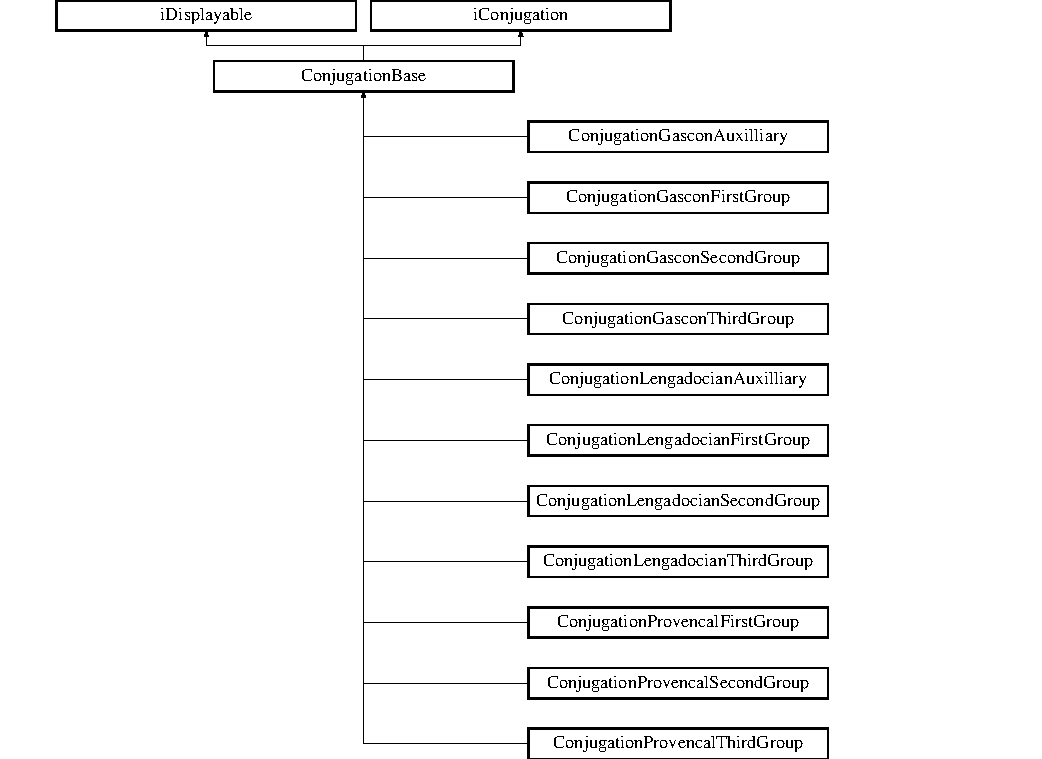
\includegraphics[height=10.196078cm]{classConjugationBase}
\end{center}
\end{figure}
\subsection*{Fonctions membres publiques}
\begin{DoxyCompactItemize}
\item 
\hyperlink{classConjugationBase_aff646e04e878c9dd1473de4619fe1bcc}{\+\_\+\+\_\+construct} (\hyperlink{classConjugationManagerBase}{Conjugation\+Manager\+Base} \$manager)
\begin{DoxyCompactList}\small\item\em Constructor. \end{DoxyCompactList}\item 
\hyperlink{classConjugationBase_a8137cfd9e8f57dafedd5cc724d57b9e6}{conjugate} ()
\begin{DoxyCompactList}\small\item\em builds an associative array w/ all informations processed by the conjugation manager \end{DoxyCompactList}\item 
\hyperlink{classConjugationBase_aa88c93007f333b916a6a51819e50e8ae}{get\+Group} ()
\item 
\hyperlink{classConjugationBase_a732cbfda6f4c28efeec68fc85aa9b65a}{get\+Verb} ()
\item 
\hyperlink{classConjugationBase_aaa7ecb3341682d48f2d2b42810de2ac2}{get\+Verb\+Model} ()
\item 
\hyperlink{classConjugationBase_a31a6fb3f63b144c6d9f0e9a27d3d28cc}{get\+Verb\+Model\+Object} (\$nummodel)
\item 
\hyperlink{classConjugationBase_a52db22137154c2fd7a8487406b959652}{getlib\+Model} ()
\item 
\hyperlink{classConjugationBase_ac381d5a6d6411aba279cb56e8505bb30}{get\+Comments} ()
\item 
\hyperlink{classConjugationBase_aab285eff4995c059a3aa0abec778a390}{get\+Manager} ()
\item 
\hyperlink{classConjugationBase_a918aff5acf4210cf363a13cf39e2430d}{get\+Verb\+Id} ()
\item 
\hyperlink{classConjugationBase_a27cc8f5f2a3b502e48c22a5b547181ac}{get\+Localization} ()
\item 
\hyperlink{classConjugationBase_ac8266b933fde0f494a7933c4d2fe0590}{get\+Alias} ()
\item 
\hyperlink{classConjugationBase_a76d7179c150a4e32fb410d5af9bc388c}{get\+See\+Also} ()
\item 
\hyperlink{classConjugationBase_a5010621a363fcfe26e5d23ade06d2c41}{get\+Dialect} ()
\item 
\hyperlink{classConjugationBase_ae5b10d1201dfc7ed1c56b1f5a073bbdb}{get\+Conjugations} ()
\item 
\hyperlink{classConjugationBase_aae493e154b07045a3ea072760ac44ef4}{get\+Dictionary\+Definition} ()
\begin{DoxyCompactList}\small\item\em asks the manager the verb definition from a dictionary \end{DoxyCompactList}\item 
\hyperlink{classConjugationBase_a0a30ad37c192a95d0986b77999a2ce5d}{get\+Row} ()
\item 
\hyperlink{classConjugationBase_a7a50c953a3f949a7740d3fb51c4b929d}{display} ()
\end{DoxyCompactItemize}
\subsection*{Attributs publics}
\begin{DoxyCompactItemize}
\item 
const \hyperlink{classConjugationBase_aa6a9ad231bf385e0bd9e240213facf36}{L\+E\+N\+G\+T\+H\+\_\+\+C\+O\+N\+J\+U\+G\+A\+T\+I\+O\+N\+\_\+\+A\+R\+R\+AY} = 11
\begin{DoxyCompactList}\small\item\em List of constants for the indexes. \end{DoxyCompactList}\item 
const \hyperlink{classConjugationBase_a4b8516bbdb1525fc811738abeed0e1ff}{I\+N\+D\+\_\+\+P\+R\+E\+S\+E\+NT} = 0
\item 
const \hyperlink{classConjugationBase_aff9c382a23aa5533dfed3be1f01a6b2f}{I\+N\+D\+\_\+\+I\+M\+P\+E\+R\+F\+E\+CT} = 1
\item 
const \hyperlink{classConjugationBase_a479f338d318e0c399b20e66ecd7a03ad}{I\+N\+D\+\_\+\+P\+R\+E\+T\+E\+R\+IT} = 2
\item 
const \hyperlink{classConjugationBase_ac25ac0244050e86a405bbf6fa9043a3e}{I\+N\+D\+\_\+\+F\+U\+T\+U\+RE} = 3
\item 
const \hyperlink{classConjugationBase_abfe86b2588be8dc7fc44f29a4dae0641}{I\+N\+F\+I\+N\+I\+T\+I\+VE} = 4
\item 
const \hyperlink{classConjugationBase_ace9d609af36ad729f01d6534c81caf4c}{G\+E\+R\+U\+ND} = 5
\item 
const \hyperlink{classConjugationBase_aae5feaa02f682a7e2638f2bab47e6464}{P\+A\+S\+T\+\_\+\+P\+A\+R\+T\+I\+C\+I\+P\+LE} = 6
\item 
const \hyperlink{classConjugationBase_ae4ec99d52ae2e6edd912cf67e78442bb}{I\+M\+P\+E\+R\+A\+T\+I\+VE} = 7
\item 
const \hyperlink{classConjugationBase_a143faefe023f7f45d77ad739b8611d45}{S\+U\+B\+J\+\_\+\+P\+R\+E\+S\+E\+NT} = 8
\item 
const \hyperlink{classConjugationBase_a530c57d644601e5430c7c3ffe064f705}{S\+U\+B\+J\+\_\+\+I\+M\+P\+E\+R\+F\+E\+CT} = 9
\item 
const \hyperlink{classConjugationBase_aac0359d9a8bb66ea04612b7f14d43c50}{C\+O\+N\+D\+I\+T\+I\+O\+N\+AL} = 10
\item 
const \hyperlink{classConjugationBase_ab0751622af68b3908a8c1426e42994e3}{E\+\_\+\+F\+I\+R\+ST} = 20
\item 
const \hyperlink{classConjugationBase_a5503d31ee48719d33098591810fc3f58}{E\+\_\+\+I\+N\+D\+\_\+\+P\+R\+E\+T\+E\+R\+IT} = 22
\item 
const \hyperlink{classConjugationBase_afc268d8825396ff04f01d85deaf8c33f}{E\+\_\+\+S\+U\+B\+J\+\_\+\+I\+M\+P\+E\+R\+F\+E\+CT} = 29
\item 
const \hyperlink{classConjugationBase_a9bc888695350391f4d6da8fc191679c4}{E\+\_\+\+C\+O\+N\+D\+I\+T\+I\+O\+N\+AL} = 30
\item 
const \hyperlink{classConjugationBase_a109b61ea3f44b885131acc8cd2cc1041}{N\+\_\+\+F\+I\+R\+ST} = 40
\item 
const \hyperlink{classConjugationBase_ace5ce9108e8d34a8111cd51dbe9c3598}{N\+\_\+\+I\+N\+D\+\_\+\+P\+R\+E\+T\+E\+R\+IT} = 42
\item 
const \hyperlink{classConjugationBase_a4b0123c72fd74dfbfd3fa42d71bd7e39}{N\+\_\+\+S\+U\+B\+J\+\_\+\+I\+M\+P\+E\+R\+F\+E\+CT} = 49
\item 
const \hyperlink{classConjugationBase_a66898e8176a1e2c5aacad8657b90df08}{N\+\_\+\+C\+O\+N\+D\+I\+T\+I\+O\+N\+AL} = 40
\item 
const \hyperlink{classConjugationBase_aadfcc5e449ab900e86244bcfdd8add79}{S\+W\+\_\+\+F\+I\+R\+ST} = 60
\item 
const \hyperlink{classConjugationBase_ac632d52e6076cf1bb490c82291d4c76f}{P\+\_\+\+F\+I\+R\+ST} = 80
\item 
const \hyperlink{classConjugationBase_a997e57538ff7276bae361d1333f11d11}{A\+U\+X\+I\+L\+L\+I\+A\+RY} = 0
\item 
const \hyperlink{classConjugationBase_a98dfd89993e82fd8bd1cc855dac980fc}{F\+I\+R\+S\+T\+\_\+\+G\+R\+O\+UP} = 1
\item 
const \hyperlink{classConjugationBase_aed0c839ab301efe958079fac4bc96811}{S\+E\+C\+O\+N\+D\+\_\+\+G\+R\+O\+UP} = 2
\item 
const \hyperlink{classConjugationBase_a15fb84852952c270f80139517000d263}{T\+H\+I\+R\+D\+\_\+\+G\+R\+O\+UP} = 3
\item 
const \hyperlink{classConjugationBase_a611f1018ef9d7b1fb76ef25864bc09b9}{L\+A\+S\+T\+\_\+\+N\+O\+R\+M\+A\+L\+\_\+\+T\+E\+M\+PS} = \hyperlink{classConjugationBase_aac0359d9a8bb66ea04612b7f14d43c50}{Conjugation\+Base\+::\+C\+O\+N\+D\+I\+T\+I\+O\+N\+AL}
\end{DoxyCompactItemize}
\subsection*{Fonctions membres protégées}
\begin{DoxyCompactItemize}
\item 
\hyperlink{classConjugationBase_af8a92808eec27a866fe83fe64ba10784}{is\+Vowel\+Detected} (\$root)
\begin{DoxyCompactList}\small\item\em a vowel detector \end{DoxyCompactList}\item 
\hyperlink{classConjugationBase_a5fd0cc4d15523febc5eabfc41d8bdb21}{is\+Tonic\+Detected} (\$root)
\begin{DoxyCompactList}\small\item\em vowel accentuated as tonic \end{DoxyCompactList}\item 
\hyperlink{classConjugationBase_a7d66d915461d677c63117166cb85e813}{neutralize\+Vowel} (\$infinitive, \$vowel\+Grave)
\begin{DoxyCompactList}\small\item\em neutralize the accent \end{DoxyCompactList}\item 
\hyperlink{classConjugationBase_a4fa62e858acfcf5eb83c11645687690c}{neutralize\+Tonic} (\$infinitive, \$tonic)
\begin{DoxyCompactList}\small\item\em neutralizes the tonic accent \end{DoxyCompactList}\item 
\hyperlink{classConjugationBase_aeaff0cedbe91b8a5cd534401d3b3ed74}{must\+Neutralize\+Vowel} (\$temps, \$person)
\begin{DoxyCompactList}\small\item\em tells if the accent must be neutralized \end{DoxyCompactList}\item 
\hyperlink{classConjugationBase_a4e623e786e39aecdaf26913685f9f040}{phonologic\+Fixes} (\$string)
\begin{DoxyCompactList}\small\item\em fixes a string according to the occitan phonologic rules \end{DoxyCompactList}\item 
\hyperlink{classConjugationBase_ab55301132f0c90c3b5bf7f6cb44fc6b4}{fix\+Radical} (\$radical, \$desinence)
\begin{DoxyCompactList}\small\item\em dummy function \end{DoxyCompactList}\item 
\hyperlink{classConjugationBase_ab983db20dcc0f19fdce07fd4a8fdbc18}{fix\+Desinence} (\$desinence)
\begin{DoxyCompactList}\small\item\em dummy function \end{DoxyCompactList}\item 
\hyperlink{classConjugationBase_a9b0524f2dde45dcdc8f6c27d673c827a}{get\+Desinence\+Length\+Array} ()
\begin{DoxyCompactList}\small\item\em dummy function \end{DoxyCompactList}\item 
\hyperlink{classConjugationBase_a97684bf47a4b158a2d4f5716f9187730}{get\+Standard\+Conjugation} ()
\begin{DoxyCompactList}\small\item\em dummy function \end{DoxyCompactList}\item 
\hyperlink{classConjugationBase_a4358d211e7c70a82657e5418a554a555}{get\+Conjugation\+Array} ()
\end{DoxyCompactItemize}


\subsection{Documentation des constructeurs et destructeur}
\hypertarget{classConjugationBase_aff646e04e878c9dd1473de4619fe1bcc}{}\label{classConjugationBase_aff646e04e878c9dd1473de4619fe1bcc} 
\index{Conjugation\+Base@{Conjugation\+Base}!\+\_\+\+\_\+construct@{\+\_\+\+\_\+construct}}
\index{\+\_\+\+\_\+construct@{\+\_\+\+\_\+construct}!Conjugation\+Base@{Conjugation\+Base}}
\subsubsection{\texorpdfstring{\+\_\+\+\_\+construct()}{\_\_construct()}}
{\footnotesize\ttfamily Conjugation\+Base\+::\+\_\+\+\_\+construct (\begin{DoxyParamCaption}\item[{\hyperlink{classConjugationManagerBase}{Conjugation\+Manager\+Base}}]{\$manager }\end{DoxyParamCaption})}



Constructor. 

points to the manager


\begin{DoxyParams}{Paramètres}
{\em \$manager} & the conjugation mananager. \\
\hline
\end{DoxyParams}
\begin{DoxyReturn}{Renvoie}
\hyperlink{classConjugationBase}{Conjugation\+Base} object. 
\end{DoxyReturn}


\subsection{Documentation des fonctions membres}
\hypertarget{classConjugationBase_a8137cfd9e8f57dafedd5cc724d57b9e6}{}\label{classConjugationBase_a8137cfd9e8f57dafedd5cc724d57b9e6} 
\index{Conjugation\+Base@{Conjugation\+Base}!conjugate@{conjugate}}
\index{conjugate@{conjugate}!Conjugation\+Base@{Conjugation\+Base}}
\subsubsection{\texorpdfstring{conjugate()}{conjugate()}}
{\footnotesize\ttfamily Conjugation\+Base\+::conjugate (\begin{DoxyParamCaption}{ }\end{DoxyParamCaption})}



builds an associative array w/ all informations processed by the conjugation manager 

gets all the information from the manager

\begin{DoxyReturn}{Renvoie}
the associative array for the conjugation 
\end{DoxyReturn}
\hypertarget{classConjugationBase_a7a50c953a3f949a7740d3fb51c4b929d}{}\label{classConjugationBase_a7a50c953a3f949a7740d3fb51c4b929d} 
\index{Conjugation\+Base@{Conjugation\+Base}!display@{display}}
\index{display@{display}!Conjugation\+Base@{Conjugation\+Base}}
\subsubsection{\texorpdfstring{display()}{display()}}
{\footnotesize\ttfamily Conjugation\+Base\+::display (\begin{DoxyParamCaption}{ }\end{DoxyParamCaption})\hspace{0.3cm}{\ttfamily [abstract]}}

differs the implementation to the descendants 

Implémente \hyperlink{interfaceiDisplayable}{i\+Displayable}.

\hypertarget{classConjugationBase_ab983db20dcc0f19fdce07fd4a8fdbc18}{}\label{classConjugationBase_ab983db20dcc0f19fdce07fd4a8fdbc18} 
\index{Conjugation\+Base@{Conjugation\+Base}!fix\+Desinence@{fix\+Desinence}}
\index{fix\+Desinence@{fix\+Desinence}!Conjugation\+Base@{Conjugation\+Base}}
\subsubsection{\texorpdfstring{fix\+Desinence()}{fixDesinence()}}
{\footnotesize\ttfamily Conjugation\+Base\+::fix\+Desinence (\begin{DoxyParamCaption}\item[{}]{\$desinence }\end{DoxyParamCaption})\hspace{0.3cm}{\ttfamily [protected]}}



dummy function 

does nothing


\begin{DoxyParams}{Paramètres}
{\em \$desinence} & \\
\hline
\end{DoxyParams}
\begin{DoxyReturn}{Renvoie}
the desinence 
\end{DoxyReturn}
\hypertarget{classConjugationBase_ab55301132f0c90c3b5bf7f6cb44fc6b4}{}\label{classConjugationBase_ab55301132f0c90c3b5bf7f6cb44fc6b4} 
\index{Conjugation\+Base@{Conjugation\+Base}!fix\+Radical@{fix\+Radical}}
\index{fix\+Radical@{fix\+Radical}!Conjugation\+Base@{Conjugation\+Base}}
\subsubsection{\texorpdfstring{fix\+Radical()}{fixRadical()}}
{\footnotesize\ttfamily Conjugation\+Base\+::fix\+Radical (\begin{DoxyParamCaption}\item[{}]{\$radical,  }\item[{}]{\$desinence }\end{DoxyParamCaption})\hspace{0.3cm}{\ttfamily [protected]}}



dummy function 

does nothing


\begin{DoxyParams}{Paramètres}
{\em \$radical} & \\
\hline
{\em \$desinence} & \\
\hline
\end{DoxyParams}
\begin{DoxyReturn}{Renvoie}
the radical 
\end{DoxyReturn}
\hypertarget{classConjugationBase_ac8266b933fde0f494a7933c4d2fe0590}{}\label{classConjugationBase_ac8266b933fde0f494a7933c4d2fe0590} 
\index{Conjugation\+Base@{Conjugation\+Base}!get\+Alias@{get\+Alias}}
\index{get\+Alias@{get\+Alias}!Conjugation\+Base@{Conjugation\+Base}}
\subsubsection{\texorpdfstring{get\+Alias()}{getAlias()}}
{\footnotesize\ttfamily Conjugation\+Base\+::get\+Alias (\begin{DoxyParamCaption}{ }\end{DoxyParamCaption})}

accessor to a manager method 

Implémente \hyperlink{interfaceiConjugation_a30a8959865d6b8d3f4ae69c31792f32a}{i\+Conjugation}.

\hypertarget{classConjugationBase_ac381d5a6d6411aba279cb56e8505bb30}{}\label{classConjugationBase_ac381d5a6d6411aba279cb56e8505bb30} 
\index{Conjugation\+Base@{Conjugation\+Base}!get\+Comments@{get\+Comments}}
\index{get\+Comments@{get\+Comments}!Conjugation\+Base@{Conjugation\+Base}}
\subsubsection{\texorpdfstring{get\+Comments()}{getComments()}}
{\footnotesize\ttfamily Conjugation\+Base\+::get\+Comments (\begin{DoxyParamCaption}{ }\end{DoxyParamCaption})}

accessor to a manager method 

Implémente \hyperlink{interfaceiConjugation}{i\+Conjugation}.

\hypertarget{classConjugationBase_a4358d211e7c70a82657e5418a554a555}{}\label{classConjugationBase_a4358d211e7c70a82657e5418a554a555} 
\index{Conjugation\+Base@{Conjugation\+Base}!get\+Conjugation\+Array@{get\+Conjugation\+Array}}
\index{get\+Conjugation\+Array@{get\+Conjugation\+Array}!Conjugation\+Base@{Conjugation\+Base}}
\subsubsection{\texorpdfstring{get\+Conjugation\+Array()}{getConjugationArray()}}
{\footnotesize\ttfamily Conjugation\+Base\+::get\+Conjugation\+Array (\begin{DoxyParamCaption}{ }\end{DoxyParamCaption})\hspace{0.3cm}{\ttfamily [abstract]}, {\ttfamily [protected]}}

differs the implementation to the descendants \hypertarget{classConjugationBase_ae5b10d1201dfc7ed1c56b1f5a073bbdb}{}\label{classConjugationBase_ae5b10d1201dfc7ed1c56b1f5a073bbdb} 
\index{Conjugation\+Base@{Conjugation\+Base}!get\+Conjugations@{get\+Conjugations}}
\index{get\+Conjugations@{get\+Conjugations}!Conjugation\+Base@{Conjugation\+Base}}
\subsubsection{\texorpdfstring{get\+Conjugations()}{getConjugations()}}
{\footnotesize\ttfamily Conjugation\+Base\+::get\+Conjugations (\begin{DoxyParamCaption}{ }\end{DoxyParamCaption})}

accessor to a manager method 

Implémente \hyperlink{interfaceiConjugation_a6c0072d898eb8b2f3756c87dfed4af33}{i\+Conjugation}.

\hypertarget{classConjugationBase_a9b0524f2dde45dcdc8f6c27d673c827a}{}\label{classConjugationBase_a9b0524f2dde45dcdc8f6c27d673c827a} 
\index{Conjugation\+Base@{Conjugation\+Base}!get\+Desinence\+Length\+Array@{get\+Desinence\+Length\+Array}}
\index{get\+Desinence\+Length\+Array@{get\+Desinence\+Length\+Array}!Conjugation\+Base@{Conjugation\+Base}}
\subsubsection{\texorpdfstring{get\+Desinence\+Length\+Array()}{getDesinenceLengthArray()}}
{\footnotesize\ttfamily Conjugation\+Base\+::get\+Desinence\+Length\+Array (\begin{DoxyParamCaption}{ }\end{DoxyParamCaption})\hspace{0.3cm}{\ttfamily [protected]}}



dummy function 

does nothing

\begin{DoxyReturn}{Renvoie}
the desinence lengths array 
\end{DoxyReturn}
\hypertarget{classConjugationBase_a5010621a363fcfe26e5d23ade06d2c41}{}\label{classConjugationBase_a5010621a363fcfe26e5d23ade06d2c41} 
\index{Conjugation\+Base@{Conjugation\+Base}!get\+Dialect@{get\+Dialect}}
\index{get\+Dialect@{get\+Dialect}!Conjugation\+Base@{Conjugation\+Base}}
\subsubsection{\texorpdfstring{get\+Dialect()}{getDialect()}}
{\footnotesize\ttfamily Conjugation\+Base\+::get\+Dialect (\begin{DoxyParamCaption}{ }\end{DoxyParamCaption})}

accessor to a manager method 

Implémente \hyperlink{interfaceiConjugation_a4e0b6c0923ecd596b6acff6c7b776f5f}{i\+Conjugation}.

\hypertarget{classConjugationBase_aae493e154b07045a3ea072760ac44ef4}{}\label{classConjugationBase_aae493e154b07045a3ea072760ac44ef4} 
\index{Conjugation\+Base@{Conjugation\+Base}!get\+Dictionary\+Definition@{get\+Dictionary\+Definition}}
\index{get\+Dictionary\+Definition@{get\+Dictionary\+Definition}!Conjugation\+Base@{Conjugation\+Base}}
\subsubsection{\texorpdfstring{get\+Dictionary\+Definition()}{getDictionaryDefinition()}}
{\footnotesize\ttfamily Conjugation\+Base\+::get\+Dictionary\+Definition (\begin{DoxyParamCaption}{ }\end{DoxyParamCaption})}



asks the manager the verb definition from a dictionary 

gets the infinitive and passes it to the manager method to seek the dictionary definition

\begin{DoxyReturn}{Renvoie}
the dictionary definition 
\end{DoxyReturn}


Implémente \hyperlink{interfaceiConjugation_ab13cedc1b4f0d064a9bfff3cbfb63de6}{i\+Conjugation}.

\hypertarget{classConjugationBase_aa88c93007f333b916a6a51819e50e8ae}{}\label{classConjugationBase_aa88c93007f333b916a6a51819e50e8ae} 
\index{Conjugation\+Base@{Conjugation\+Base}!get\+Group@{get\+Group}}
\index{get\+Group@{get\+Group}!Conjugation\+Base@{Conjugation\+Base}}
\subsubsection{\texorpdfstring{get\+Group()}{getGroup()}}
{\footnotesize\ttfamily Conjugation\+Base\+::get\+Group (\begin{DoxyParamCaption}{ }\end{DoxyParamCaption})}

accessor to a manager method 

Implémente \hyperlink{interfaceiConjugation_a21390064de33a77b99b26ec5a2e55351}{i\+Conjugation}.

\hypertarget{classConjugationBase_a52db22137154c2fd7a8487406b959652}{}\label{classConjugationBase_a52db22137154c2fd7a8487406b959652} 
\index{Conjugation\+Base@{Conjugation\+Base}!getlib\+Model@{getlib\+Model}}
\index{getlib\+Model@{getlib\+Model}!Conjugation\+Base@{Conjugation\+Base}}
\subsubsection{\texorpdfstring{getlib\+Model()}{getlibModel()}}
{\footnotesize\ttfamily Conjugation\+Base\+::getlib\+Model (\begin{DoxyParamCaption}{ }\end{DoxyParamCaption})}

accessor to a manager method 

Implémente \hyperlink{interfaceiConjugation_a2b6dd0a979a98bc50f6f9f7ec9b69e63}{i\+Conjugation}.

\hypertarget{classConjugationBase_a27cc8f5f2a3b502e48c22a5b547181ac}{}\label{classConjugationBase_a27cc8f5f2a3b502e48c22a5b547181ac} 
\index{Conjugation\+Base@{Conjugation\+Base}!get\+Localization@{get\+Localization}}
\index{get\+Localization@{get\+Localization}!Conjugation\+Base@{Conjugation\+Base}}
\subsubsection{\texorpdfstring{get\+Localization()}{getLocalization()}}
{\footnotesize\ttfamily Conjugation\+Base\+::get\+Localization (\begin{DoxyParamCaption}{ }\end{DoxyParamCaption})}

accessor to a manager method 

Implémente \hyperlink{interfaceiConjugation_ab19ceb5ab295fd3d0f862d963379a7e2}{i\+Conjugation}.

\hypertarget{classConjugationBase_aab285eff4995c059a3aa0abec778a390}{}\label{classConjugationBase_aab285eff4995c059a3aa0abec778a390} 
\index{Conjugation\+Base@{Conjugation\+Base}!get\+Manager@{get\+Manager}}
\index{get\+Manager@{get\+Manager}!Conjugation\+Base@{Conjugation\+Base}}
\subsubsection{\texorpdfstring{get\+Manager()}{getManager()}}
{\footnotesize\ttfamily Conjugation\+Base\+::get\+Manager (\begin{DoxyParamCaption}{ }\end{DoxyParamCaption})}

accessor to a manager method 

Implémente \hyperlink{interfaceiConjugation_a448829b47813a79d1f8ec65de91e8696}{i\+Conjugation}.

\hypertarget{classConjugationBase_a0a30ad37c192a95d0986b77999a2ce5d}{}\label{classConjugationBase_a0a30ad37c192a95d0986b77999a2ce5d} 
\index{Conjugation\+Base@{Conjugation\+Base}!get\+Row@{get\+Row}}
\index{get\+Row@{get\+Row}!Conjugation\+Base@{Conjugation\+Base}}
\subsubsection{\texorpdfstring{get\+Row()}{getRow()}}
{\footnotesize\ttfamily Conjugation\+Base\+::get\+Row (\begin{DoxyParamCaption}{ }\end{DoxyParamCaption})}

accessor to a manager method \hypertarget{classConjugationBase_a76d7179c150a4e32fb410d5af9bc388c}{}\label{classConjugationBase_a76d7179c150a4e32fb410d5af9bc388c} 
\index{Conjugation\+Base@{Conjugation\+Base}!get\+See\+Also@{get\+See\+Also}}
\index{get\+See\+Also@{get\+See\+Also}!Conjugation\+Base@{Conjugation\+Base}}
\subsubsection{\texorpdfstring{get\+See\+Also()}{getSeeAlso()}}
{\footnotesize\ttfamily Conjugation\+Base\+::get\+See\+Also (\begin{DoxyParamCaption}{ }\end{DoxyParamCaption})}

accessor to a manager method 

Implémente \hyperlink{interfaceiConjugation_a58e61c703ad1f0d76db1535235e530a0}{i\+Conjugation}.

\hypertarget{classConjugationBase_a97684bf47a4b158a2d4f5716f9187730}{}\label{classConjugationBase_a97684bf47a4b158a2d4f5716f9187730} 
\index{Conjugation\+Base@{Conjugation\+Base}!get\+Standard\+Conjugation@{get\+Standard\+Conjugation}}
\index{get\+Standard\+Conjugation@{get\+Standard\+Conjugation}!Conjugation\+Base@{Conjugation\+Base}}
\subsubsection{\texorpdfstring{get\+Standard\+Conjugation()}{getStandardConjugation()}}
{\footnotesize\ttfamily Conjugation\+Base\+::get\+Standard\+Conjugation (\begin{DoxyParamCaption}{ }\end{DoxyParamCaption})\hspace{0.3cm}{\ttfamily [protected]}}



dummy function 

does nothing

\begin{DoxyReturn}{Renvoie}
the standard conjugation array 
\end{DoxyReturn}
\hypertarget{classConjugationBase_a732cbfda6f4c28efeec68fc85aa9b65a}{}\label{classConjugationBase_a732cbfda6f4c28efeec68fc85aa9b65a} 
\index{Conjugation\+Base@{Conjugation\+Base}!get\+Verb@{get\+Verb}}
\index{get\+Verb@{get\+Verb}!Conjugation\+Base@{Conjugation\+Base}}
\subsubsection{\texorpdfstring{get\+Verb()}{getVerb()}}
{\footnotesize\ttfamily Conjugation\+Base\+::get\+Verb (\begin{DoxyParamCaption}{ }\end{DoxyParamCaption})}

accessor to a manager method 

Implémente \hyperlink{interfaceiConjugation}{i\+Conjugation}.

\hypertarget{classConjugationBase_a918aff5acf4210cf363a13cf39e2430d}{}\label{classConjugationBase_a918aff5acf4210cf363a13cf39e2430d} 
\index{Conjugation\+Base@{Conjugation\+Base}!get\+Verb\+Id@{get\+Verb\+Id}}
\index{get\+Verb\+Id@{get\+Verb\+Id}!Conjugation\+Base@{Conjugation\+Base}}
\subsubsection{\texorpdfstring{get\+Verb\+Id()}{getVerbId()}}
{\footnotesize\ttfamily Conjugation\+Base\+::get\+Verb\+Id (\begin{DoxyParamCaption}{ }\end{DoxyParamCaption})}

accessor to a manager method 

Implémente \hyperlink{interfaceiConjugation_aa34e7af66125d28af4f485529d456a74}{i\+Conjugation}.

\hypertarget{classConjugationBase_aaa7ecb3341682d48f2d2b42810de2ac2}{}\label{classConjugationBase_aaa7ecb3341682d48f2d2b42810de2ac2} 
\index{Conjugation\+Base@{Conjugation\+Base}!get\+Verb\+Model@{get\+Verb\+Model}}
\index{get\+Verb\+Model@{get\+Verb\+Model}!Conjugation\+Base@{Conjugation\+Base}}
\subsubsection{\texorpdfstring{get\+Verb\+Model()}{getVerbModel()}}
{\footnotesize\ttfamily Conjugation\+Base\+::get\+Verb\+Model (\begin{DoxyParamCaption}{ }\end{DoxyParamCaption})}

accessor to a manager method 

Implémente \hyperlink{interfaceiConjugation_ab5482cc8f8e9f58dc852aff604813b6e}{i\+Conjugation}.

\hypertarget{classConjugationBase_a31a6fb3f63b144c6d9f0e9a27d3d28cc}{}\label{classConjugationBase_a31a6fb3f63b144c6d9f0e9a27d3d28cc} 
\index{Conjugation\+Base@{Conjugation\+Base}!get\+Verb\+Model\+Object@{get\+Verb\+Model\+Object}}
\index{get\+Verb\+Model\+Object@{get\+Verb\+Model\+Object}!Conjugation\+Base@{Conjugation\+Base}}
\subsubsection{\texorpdfstring{get\+Verb\+Model\+Object()}{getVerbModelObject()}}
{\footnotesize\ttfamily Conjugation\+Base\+::get\+Verb\+Model\+Object (\begin{DoxyParamCaption}\item[{}]{\$nummodel }\end{DoxyParamCaption})}

accessor to a manager method 

Implémente \hyperlink{interfaceiConjugation}{i\+Conjugation}.

\hypertarget{classConjugationBase_a5fd0cc4d15523febc5eabfc41d8bdb21}{}\label{classConjugationBase_a5fd0cc4d15523febc5eabfc41d8bdb21} 
\index{Conjugation\+Base@{Conjugation\+Base}!is\+Tonic\+Detected@{is\+Tonic\+Detected}}
\index{is\+Tonic\+Detected@{is\+Tonic\+Detected}!Conjugation\+Base@{Conjugation\+Base}}
\subsubsection{\texorpdfstring{is\+Tonic\+Detected()}{isTonicDetected()}}
{\footnotesize\ttfamily Conjugation\+Base\+::is\+Tonic\+Detected (\begin{DoxyParamCaption}\item[{}]{\$root }\end{DoxyParamCaption})\hspace{0.3cm}{\ttfamily [protected]}}



vowel accentuated as tonic 

in occitan language a tonic vowel is distinguised by the accentuation


\begin{DoxyParams}{Paramètres}
{\em \$root} & the radical of the verb \\
\hline
\end{DoxyParams}
\begin{DoxyReturn}{Renvoie}
the tonic vowel detected 
\end{DoxyReturn}
\hypertarget{classConjugationBase_af8a92808eec27a866fe83fe64ba10784}{}\label{classConjugationBase_af8a92808eec27a866fe83fe64ba10784} 
\index{Conjugation\+Base@{Conjugation\+Base}!is\+Vowel\+Detected@{is\+Vowel\+Detected}}
\index{is\+Vowel\+Detected@{is\+Vowel\+Detected}!Conjugation\+Base@{Conjugation\+Base}}
\subsubsection{\texorpdfstring{is\+Vowel\+Detected()}{isVowelDetected()}}
{\footnotesize\ttfamily Conjugation\+Base\+::is\+Vowel\+Detected (\begin{DoxyParamCaption}\item[{}]{\$root }\end{DoxyParamCaption})\hspace{0.3cm}{\ttfamily [protected]}}



a vowel detector 


\begin{DoxyParams}{Paramètres}
{\em \$root} & the radical of the verb \\
\hline
\end{DoxyParams}
\begin{DoxyReturn}{Renvoie}
the vowel detected 
\end{DoxyReturn}
\hypertarget{classConjugationBase_aeaff0cedbe91b8a5cd534401d3b3ed74}{}\label{classConjugationBase_aeaff0cedbe91b8a5cd534401d3b3ed74} 
\index{Conjugation\+Base@{Conjugation\+Base}!must\+Neutralize\+Vowel@{must\+Neutralize\+Vowel}}
\index{must\+Neutralize\+Vowel@{must\+Neutralize\+Vowel}!Conjugation\+Base@{Conjugation\+Base}}
\subsubsection{\texorpdfstring{must\+Neutralize\+Vowel()}{mustNeutralizeVowel()}}
{\footnotesize\ttfamily Conjugation\+Base\+::must\+Neutralize\+Vowel (\begin{DoxyParamCaption}\item[{}]{\$temps,  }\item[{}]{\$person }\end{DoxyParamCaption})\hspace{0.3cm}{\ttfamily [protected]}}



tells if the accent must be neutralized 

takes an infinitive and remove the accent


\begin{DoxyParams}{Paramètres}
{\em \$infinitive} & \\
\hline
{\em \$vowel\+Grave} & the vowel to neutralize \\
\hline
\end{DoxyParams}
\begin{DoxyReturn}{Renvoie}
a boolean 
\end{DoxyReturn}
\hypertarget{classConjugationBase_a4fa62e858acfcf5eb83c11645687690c}{}\label{classConjugationBase_a4fa62e858acfcf5eb83c11645687690c} 
\index{Conjugation\+Base@{Conjugation\+Base}!neutralize\+Tonic@{neutralize\+Tonic}}
\index{neutralize\+Tonic@{neutralize\+Tonic}!Conjugation\+Base@{Conjugation\+Base}}
\subsubsection{\texorpdfstring{neutralize\+Tonic()}{neutralizeTonic()}}
{\footnotesize\ttfamily Conjugation\+Base\+::neutralize\+Tonic (\begin{DoxyParamCaption}\item[{}]{\$infinitive,  }\item[{}]{\$tonic }\end{DoxyParamCaption})\hspace{0.3cm}{\ttfamily [protected]}}



neutralizes the tonic accent 

takes an infinitive and remove the accent


\begin{DoxyParams}{Paramètres}
{\em \$infinitive} & \\
\hline
{\em \$vowel\+Grave} & the vowel to neutralize \\
\hline
\end{DoxyParams}
\begin{DoxyReturn}{Renvoie}
the infinitive 
\end{DoxyReturn}
\hypertarget{classConjugationBase_a7d66d915461d677c63117166cb85e813}{}\label{classConjugationBase_a7d66d915461d677c63117166cb85e813} 
\index{Conjugation\+Base@{Conjugation\+Base}!neutralize\+Vowel@{neutralize\+Vowel}}
\index{neutralize\+Vowel@{neutralize\+Vowel}!Conjugation\+Base@{Conjugation\+Base}}
\subsubsection{\texorpdfstring{neutralize\+Vowel()}{neutralizeVowel()}}
{\footnotesize\ttfamily Conjugation\+Base\+::neutralize\+Vowel (\begin{DoxyParamCaption}\item[{}]{\$infinitive,  }\item[{}]{\$vowel\+Grave }\end{DoxyParamCaption})\hspace{0.3cm}{\ttfamily [protected]}}



neutralize the accent 

takes an infinitive and remove the accent


\begin{DoxyParams}{Paramètres}
{\em \$infinitive} & \\
\hline
{\em \$vowel\+Grave} & the vowel to neutralize \\
\hline
\end{DoxyParams}
\begin{DoxyReturn}{Renvoie}
the infinitive 
\end{DoxyReturn}
\hypertarget{classConjugationBase_a4e623e786e39aecdaf26913685f9f040}{}\label{classConjugationBase_a4e623e786e39aecdaf26913685f9f040} 
\index{Conjugation\+Base@{Conjugation\+Base}!phonologic\+Fixes@{phonologic\+Fixes}}
\index{phonologic\+Fixes@{phonologic\+Fixes}!Conjugation\+Base@{Conjugation\+Base}}
\subsubsection{\texorpdfstring{phonologic\+Fixes()}{phonologicFixes()}}
{\footnotesize\ttfamily Conjugation\+Base\+::phonologic\+Fixes (\begin{DoxyParamCaption}\item[{}]{\$string }\end{DoxyParamCaption})\hspace{0.3cm}{\ttfamily [protected]}}



fixes a string according to the occitan phonologic rules 


\begin{DoxyParams}{Paramètres}
{\em \$string} & \\
\hline
\end{DoxyParams}
\begin{DoxyReturn}{Renvoie}
the string altered 
\end{DoxyReturn}


\subsection{Documentation des données membres}
\hypertarget{classConjugationBase_a997e57538ff7276bae361d1333f11d11}{}\label{classConjugationBase_a997e57538ff7276bae361d1333f11d11} 
\index{Conjugation\+Base@{Conjugation\+Base}!A\+U\+X\+I\+L\+L\+I\+A\+RY@{A\+U\+X\+I\+L\+L\+I\+A\+RY}}
\index{A\+U\+X\+I\+L\+L\+I\+A\+RY@{A\+U\+X\+I\+L\+L\+I\+A\+RY}!Conjugation\+Base@{Conjugation\+Base}}
\subsubsection{\texorpdfstring{A\+U\+X\+I\+L\+L\+I\+A\+RY}{AUXILLIARY}}
{\footnotesize\ttfamily const Conjugation\+Base\+::\+A\+U\+X\+I\+L\+L\+I\+A\+RY = 0}

V\+E\+R\+B\+AL G\+R\+O\+U\+P\+Sauxiliary \hypertarget{classConjugationBase_aac0359d9a8bb66ea04612b7f14d43c50}{}\label{classConjugationBase_aac0359d9a8bb66ea04612b7f14d43c50} 
\index{Conjugation\+Base@{Conjugation\+Base}!C\+O\+N\+D\+I\+T\+I\+O\+N\+AL@{C\+O\+N\+D\+I\+T\+I\+O\+N\+AL}}
\index{C\+O\+N\+D\+I\+T\+I\+O\+N\+AL@{C\+O\+N\+D\+I\+T\+I\+O\+N\+AL}!Conjugation\+Base@{Conjugation\+Base}}
\subsubsection{\texorpdfstring{C\+O\+N\+D\+I\+T\+I\+O\+N\+AL}{CONDITIONAL}}
{\footnotesize\ttfamily const Conjugation\+Base\+::\+C\+O\+N\+D\+I\+T\+I\+O\+N\+AL = 10}

conditional \hypertarget{classConjugationBase_a9bc888695350391f4d6da8fc191679c4}{}\label{classConjugationBase_a9bc888695350391f4d6da8fc191679c4} 
\index{Conjugation\+Base@{Conjugation\+Base}!E\+\_\+\+C\+O\+N\+D\+I\+T\+I\+O\+N\+AL@{E\+\_\+\+C\+O\+N\+D\+I\+T\+I\+O\+N\+AL}}
\index{E\+\_\+\+C\+O\+N\+D\+I\+T\+I\+O\+N\+AL@{E\+\_\+\+C\+O\+N\+D\+I\+T\+I\+O\+N\+AL}!Conjugation\+Base@{Conjugation\+Base}}
\subsubsection{\texorpdfstring{E\+\_\+\+C\+O\+N\+D\+I\+T\+I\+O\+N\+AL}{E\_CONDITIONAL}}
{\footnotesize\ttfamily const Conjugation\+Base\+::\+E\+\_\+\+C\+O\+N\+D\+I\+T\+I\+O\+N\+AL = 30}

E\+A\+S\+T\+E\+RN V\+A\+R\+I\+A\+N\+CE for C\+O\+N\+D\+I\+T\+I\+O\+N\+AL \hypertarget{classConjugationBase_ab0751622af68b3908a8c1426e42994e3}{}\label{classConjugationBase_ab0751622af68b3908a8c1426e42994e3} 
\index{Conjugation\+Base@{Conjugation\+Base}!E\+\_\+\+F\+I\+R\+ST@{E\+\_\+\+F\+I\+R\+ST}}
\index{E\+\_\+\+F\+I\+R\+ST@{E\+\_\+\+F\+I\+R\+ST}!Conjugation\+Base@{Conjugation\+Base}}
\subsubsection{\texorpdfstring{E\+\_\+\+F\+I\+R\+ST}{E\_FIRST}}
{\footnotesize\ttfamily const Conjugation\+Base\+::\+E\+\_\+\+F\+I\+R\+ST = 20}

E\+A\+ST \hypertarget{classConjugationBase_a5503d31ee48719d33098591810fc3f58}{}\label{classConjugationBase_a5503d31ee48719d33098591810fc3f58} 
\index{Conjugation\+Base@{Conjugation\+Base}!E\+\_\+\+I\+N\+D\+\_\+\+P\+R\+E\+T\+E\+R\+IT@{E\+\_\+\+I\+N\+D\+\_\+\+P\+R\+E\+T\+E\+R\+IT}}
\index{E\+\_\+\+I\+N\+D\+\_\+\+P\+R\+E\+T\+E\+R\+IT@{E\+\_\+\+I\+N\+D\+\_\+\+P\+R\+E\+T\+E\+R\+IT}!Conjugation\+Base@{Conjugation\+Base}}
\subsubsection{\texorpdfstring{E\+\_\+\+I\+N\+D\+\_\+\+P\+R\+E\+T\+E\+R\+IT}{E\_IND\_PRETERIT}}
{\footnotesize\ttfamily const Conjugation\+Base\+::\+E\+\_\+\+I\+N\+D\+\_\+\+P\+R\+E\+T\+E\+R\+IT = 22}

E\+A\+S\+T\+E\+RN V\+A\+R\+I\+A\+N\+CE for P\+R\+E\+T\+E\+R\+IT \hypertarget{classConjugationBase_afc268d8825396ff04f01d85deaf8c33f}{}\label{classConjugationBase_afc268d8825396ff04f01d85deaf8c33f} 
\index{Conjugation\+Base@{Conjugation\+Base}!E\+\_\+\+S\+U\+B\+J\+\_\+\+I\+M\+P\+E\+R\+F\+E\+CT@{E\+\_\+\+S\+U\+B\+J\+\_\+\+I\+M\+P\+E\+R\+F\+E\+CT}}
\index{E\+\_\+\+S\+U\+B\+J\+\_\+\+I\+M\+P\+E\+R\+F\+E\+CT@{E\+\_\+\+S\+U\+B\+J\+\_\+\+I\+M\+P\+E\+R\+F\+E\+CT}!Conjugation\+Base@{Conjugation\+Base}}
\subsubsection{\texorpdfstring{E\+\_\+\+S\+U\+B\+J\+\_\+\+I\+M\+P\+E\+R\+F\+E\+CT}{E\_SUBJ\_IMPERFECT}}
{\footnotesize\ttfamily const Conjugation\+Base\+::\+E\+\_\+\+S\+U\+B\+J\+\_\+\+I\+M\+P\+E\+R\+F\+E\+CT = 29}

E\+A\+S\+T\+E\+RN V\+A\+R\+I\+A\+N\+CE for S\+U\+BJ I\+M\+P\+E\+R\+F\+E\+CT \hypertarget{classConjugationBase_a98dfd89993e82fd8bd1cc855dac980fc}{}\label{classConjugationBase_a98dfd89993e82fd8bd1cc855dac980fc} 
\index{Conjugation\+Base@{Conjugation\+Base}!F\+I\+R\+S\+T\+\_\+\+G\+R\+O\+UP@{F\+I\+R\+S\+T\+\_\+\+G\+R\+O\+UP}}
\index{F\+I\+R\+S\+T\+\_\+\+G\+R\+O\+UP@{F\+I\+R\+S\+T\+\_\+\+G\+R\+O\+UP}!Conjugation\+Base@{Conjugation\+Base}}
\subsubsection{\texorpdfstring{F\+I\+R\+S\+T\+\_\+\+G\+R\+O\+UP}{FIRST\_GROUP}}
{\footnotesize\ttfamily const Conjugation\+Base\+::\+F\+I\+R\+S\+T\+\_\+\+G\+R\+O\+UP = 1}

first group \hypertarget{classConjugationBase_ace9d609af36ad729f01d6534c81caf4c}{}\label{classConjugationBase_ace9d609af36ad729f01d6534c81caf4c} 
\index{Conjugation\+Base@{Conjugation\+Base}!G\+E\+R\+U\+ND@{G\+E\+R\+U\+ND}}
\index{G\+E\+R\+U\+ND@{G\+E\+R\+U\+ND}!Conjugation\+Base@{Conjugation\+Base}}
\subsubsection{\texorpdfstring{G\+E\+R\+U\+ND}{GERUND}}
{\footnotesize\ttfamily const Conjugation\+Base\+::\+G\+E\+R\+U\+ND = 5}

mood gerundive \hypertarget{classConjugationBase_ae4ec99d52ae2e6edd912cf67e78442bb}{}\label{classConjugationBase_ae4ec99d52ae2e6edd912cf67e78442bb} 
\index{Conjugation\+Base@{Conjugation\+Base}!I\+M\+P\+E\+R\+A\+T\+I\+VE@{I\+M\+P\+E\+R\+A\+T\+I\+VE}}
\index{I\+M\+P\+E\+R\+A\+T\+I\+VE@{I\+M\+P\+E\+R\+A\+T\+I\+VE}!Conjugation\+Base@{Conjugation\+Base}}
\subsubsection{\texorpdfstring{I\+M\+P\+E\+R\+A\+T\+I\+VE}{IMPERATIVE}}
{\footnotesize\ttfamily const Conjugation\+Base\+::\+I\+M\+P\+E\+R\+A\+T\+I\+VE = 7}

mood imperative \hypertarget{classConjugationBase_ac25ac0244050e86a405bbf6fa9043a3e}{}\label{classConjugationBase_ac25ac0244050e86a405bbf6fa9043a3e} 
\index{Conjugation\+Base@{Conjugation\+Base}!I\+N\+D\+\_\+\+F\+U\+T\+U\+RE@{I\+N\+D\+\_\+\+F\+U\+T\+U\+RE}}
\index{I\+N\+D\+\_\+\+F\+U\+T\+U\+RE@{I\+N\+D\+\_\+\+F\+U\+T\+U\+RE}!Conjugation\+Base@{Conjugation\+Base}}
\subsubsection{\texorpdfstring{I\+N\+D\+\_\+\+F\+U\+T\+U\+RE}{IND\_FUTURE}}
{\footnotesize\ttfamily const Conjugation\+Base\+::\+I\+N\+D\+\_\+\+F\+U\+T\+U\+RE = 3}

indicative future \hypertarget{classConjugationBase_aff9c382a23aa5533dfed3be1f01a6b2f}{}\label{classConjugationBase_aff9c382a23aa5533dfed3be1f01a6b2f} 
\index{Conjugation\+Base@{Conjugation\+Base}!I\+N\+D\+\_\+\+I\+M\+P\+E\+R\+F\+E\+CT@{I\+N\+D\+\_\+\+I\+M\+P\+E\+R\+F\+E\+CT}}
\index{I\+N\+D\+\_\+\+I\+M\+P\+E\+R\+F\+E\+CT@{I\+N\+D\+\_\+\+I\+M\+P\+E\+R\+F\+E\+CT}!Conjugation\+Base@{Conjugation\+Base}}
\subsubsection{\texorpdfstring{I\+N\+D\+\_\+\+I\+M\+P\+E\+R\+F\+E\+CT}{IND\_IMPERFECT}}
{\footnotesize\ttfamily const Conjugation\+Base\+::\+I\+N\+D\+\_\+\+I\+M\+P\+E\+R\+F\+E\+CT = 1}

indicative imperfect \hypertarget{classConjugationBase_a4b8516bbdb1525fc811738abeed0e1ff}{}\label{classConjugationBase_a4b8516bbdb1525fc811738abeed0e1ff} 
\index{Conjugation\+Base@{Conjugation\+Base}!I\+N\+D\+\_\+\+P\+R\+E\+S\+E\+NT@{I\+N\+D\+\_\+\+P\+R\+E\+S\+E\+NT}}
\index{I\+N\+D\+\_\+\+P\+R\+E\+S\+E\+NT@{I\+N\+D\+\_\+\+P\+R\+E\+S\+E\+NT}!Conjugation\+Base@{Conjugation\+Base}}
\subsubsection{\texorpdfstring{I\+N\+D\+\_\+\+P\+R\+E\+S\+E\+NT}{IND\_PRESENT}}
{\footnotesize\ttfamily const Conjugation\+Base\+::\+I\+N\+D\+\_\+\+P\+R\+E\+S\+E\+NT = 0}

indicative present \hypertarget{classConjugationBase_a479f338d318e0c399b20e66ecd7a03ad}{}\label{classConjugationBase_a479f338d318e0c399b20e66ecd7a03ad} 
\index{Conjugation\+Base@{Conjugation\+Base}!I\+N\+D\+\_\+\+P\+R\+E\+T\+E\+R\+IT@{I\+N\+D\+\_\+\+P\+R\+E\+T\+E\+R\+IT}}
\index{I\+N\+D\+\_\+\+P\+R\+E\+T\+E\+R\+IT@{I\+N\+D\+\_\+\+P\+R\+E\+T\+E\+R\+IT}!Conjugation\+Base@{Conjugation\+Base}}
\subsubsection{\texorpdfstring{I\+N\+D\+\_\+\+P\+R\+E\+T\+E\+R\+IT}{IND\_PRETERIT}}
{\footnotesize\ttfamily const Conjugation\+Base\+::\+I\+N\+D\+\_\+\+P\+R\+E\+T\+E\+R\+IT = 2}

indicative preterit \hypertarget{classConjugationBase_abfe86b2588be8dc7fc44f29a4dae0641}{}\label{classConjugationBase_abfe86b2588be8dc7fc44f29a4dae0641} 
\index{Conjugation\+Base@{Conjugation\+Base}!I\+N\+F\+I\+N\+I\+T\+I\+VE@{I\+N\+F\+I\+N\+I\+T\+I\+VE}}
\index{I\+N\+F\+I\+N\+I\+T\+I\+VE@{I\+N\+F\+I\+N\+I\+T\+I\+VE}!Conjugation\+Base@{Conjugation\+Base}}
\subsubsection{\texorpdfstring{I\+N\+F\+I\+N\+I\+T\+I\+VE}{INFINITIVE}}
{\footnotesize\ttfamily const Conjugation\+Base\+::\+I\+N\+F\+I\+N\+I\+T\+I\+VE = 4}

mood infinitive \hypertarget{classConjugationBase_a611f1018ef9d7b1fb76ef25864bc09b9}{}\label{classConjugationBase_a611f1018ef9d7b1fb76ef25864bc09b9} 
\index{Conjugation\+Base@{Conjugation\+Base}!L\+A\+S\+T\+\_\+\+N\+O\+R\+M\+A\+L\+\_\+\+T\+E\+M\+PS@{L\+A\+S\+T\+\_\+\+N\+O\+R\+M\+A\+L\+\_\+\+T\+E\+M\+PS}}
\index{L\+A\+S\+T\+\_\+\+N\+O\+R\+M\+A\+L\+\_\+\+T\+E\+M\+PS@{L\+A\+S\+T\+\_\+\+N\+O\+R\+M\+A\+L\+\_\+\+T\+E\+M\+PS}!Conjugation\+Base@{Conjugation\+Base}}
\subsubsection{\texorpdfstring{L\+A\+S\+T\+\_\+\+N\+O\+R\+M\+A\+L\+\_\+\+T\+E\+M\+PS}{LAST\_NORMAL\_TEMPS}}
{\footnotesize\ttfamily const Conjugation\+Base\+::\+L\+A\+S\+T\+\_\+\+N\+O\+R\+M\+A\+L\+\_\+\+T\+E\+M\+PS = \hyperlink{classConjugationBase_aac0359d9a8bb66ea04612b7f14d43c50}{Conjugation\+Base\+::\+C\+O\+N\+D\+I\+T\+I\+O\+N\+AL}}

the end binding \hypertarget{classConjugationBase_aa6a9ad231bf385e0bd9e240213facf36}{}\label{classConjugationBase_aa6a9ad231bf385e0bd9e240213facf36} 
\index{Conjugation\+Base@{Conjugation\+Base}!L\+E\+N\+G\+T\+H\+\_\+\+C\+O\+N\+J\+U\+G\+A\+T\+I\+O\+N\+\_\+\+A\+R\+R\+AY@{L\+E\+N\+G\+T\+H\+\_\+\+C\+O\+N\+J\+U\+G\+A\+T\+I\+O\+N\+\_\+\+A\+R\+R\+AY}}
\index{L\+E\+N\+G\+T\+H\+\_\+\+C\+O\+N\+J\+U\+G\+A\+T\+I\+O\+N\+\_\+\+A\+R\+R\+AY@{L\+E\+N\+G\+T\+H\+\_\+\+C\+O\+N\+J\+U\+G\+A\+T\+I\+O\+N\+\_\+\+A\+R\+R\+AY}!Conjugation\+Base@{Conjugation\+Base}}
\subsubsection{\texorpdfstring{L\+E\+N\+G\+T\+H\+\_\+\+C\+O\+N\+J\+U\+G\+A\+T\+I\+O\+N\+\_\+\+A\+R\+R\+AY}{LENGTH\_CONJUGATION\_ARRAY}}
{\footnotesize\ttfamily const Conjugation\+Base\+::\+L\+E\+N\+G\+T\+H\+\_\+\+C\+O\+N\+J\+U\+G\+A\+T\+I\+O\+N\+\_\+\+A\+R\+R\+AY = 11}



List of constants for the indexes. 

Indexes of an arrray returned by the conjugation processor Tempses and some geographical variances for gascon dialect \hypertarget{classConjugationBase_a66898e8176a1e2c5aacad8657b90df08}{}\label{classConjugationBase_a66898e8176a1e2c5aacad8657b90df08} 
\index{Conjugation\+Base@{Conjugation\+Base}!N\+\_\+\+C\+O\+N\+D\+I\+T\+I\+O\+N\+AL@{N\+\_\+\+C\+O\+N\+D\+I\+T\+I\+O\+N\+AL}}
\index{N\+\_\+\+C\+O\+N\+D\+I\+T\+I\+O\+N\+AL@{N\+\_\+\+C\+O\+N\+D\+I\+T\+I\+O\+N\+AL}!Conjugation\+Base@{Conjugation\+Base}}
\subsubsection{\texorpdfstring{N\+\_\+\+C\+O\+N\+D\+I\+T\+I\+O\+N\+AL}{N\_CONDITIONAL}}
{\footnotesize\ttfamily const Conjugation\+Base\+::\+N\+\_\+\+C\+O\+N\+D\+I\+T\+I\+O\+N\+AL = 40}

N\+O\+R\+T\+H\+E\+RN V\+A\+R\+I\+A\+N\+CE for C\+O\+N\+D\+I\+T\+I\+O\+N\+AL \hypertarget{classConjugationBase_a109b61ea3f44b885131acc8cd2cc1041}{}\label{classConjugationBase_a109b61ea3f44b885131acc8cd2cc1041} 
\index{Conjugation\+Base@{Conjugation\+Base}!N\+\_\+\+F\+I\+R\+ST@{N\+\_\+\+F\+I\+R\+ST}}
\index{N\+\_\+\+F\+I\+R\+ST@{N\+\_\+\+F\+I\+R\+ST}!Conjugation\+Base@{Conjugation\+Base}}
\subsubsection{\texorpdfstring{N\+\_\+\+F\+I\+R\+ST}{N\_FIRST}}
{\footnotesize\ttfamily const Conjugation\+Base\+::\+N\+\_\+\+F\+I\+R\+ST = 40}

N\+O\+R\+TH \hypertarget{classConjugationBase_ace5ce9108e8d34a8111cd51dbe9c3598}{}\label{classConjugationBase_ace5ce9108e8d34a8111cd51dbe9c3598} 
\index{Conjugation\+Base@{Conjugation\+Base}!N\+\_\+\+I\+N\+D\+\_\+\+P\+R\+E\+T\+E\+R\+IT@{N\+\_\+\+I\+N\+D\+\_\+\+P\+R\+E\+T\+E\+R\+IT}}
\index{N\+\_\+\+I\+N\+D\+\_\+\+P\+R\+E\+T\+E\+R\+IT@{N\+\_\+\+I\+N\+D\+\_\+\+P\+R\+E\+T\+E\+R\+IT}!Conjugation\+Base@{Conjugation\+Base}}
\subsubsection{\texorpdfstring{N\+\_\+\+I\+N\+D\+\_\+\+P\+R\+E\+T\+E\+R\+IT}{N\_IND\_PRETERIT}}
{\footnotesize\ttfamily const Conjugation\+Base\+::\+N\+\_\+\+I\+N\+D\+\_\+\+P\+R\+E\+T\+E\+R\+IT = 42}

N\+O\+R\+T\+H\+E\+RN V\+A\+R\+I\+A\+N\+CE for P\+R\+E\+T\+E\+R\+IT \hypertarget{classConjugationBase_a4b0123c72fd74dfbfd3fa42d71bd7e39}{}\label{classConjugationBase_a4b0123c72fd74dfbfd3fa42d71bd7e39} 
\index{Conjugation\+Base@{Conjugation\+Base}!N\+\_\+\+S\+U\+B\+J\+\_\+\+I\+M\+P\+E\+R\+F\+E\+CT@{N\+\_\+\+S\+U\+B\+J\+\_\+\+I\+M\+P\+E\+R\+F\+E\+CT}}
\index{N\+\_\+\+S\+U\+B\+J\+\_\+\+I\+M\+P\+E\+R\+F\+E\+CT@{N\+\_\+\+S\+U\+B\+J\+\_\+\+I\+M\+P\+E\+R\+F\+E\+CT}!Conjugation\+Base@{Conjugation\+Base}}
\subsubsection{\texorpdfstring{N\+\_\+\+S\+U\+B\+J\+\_\+\+I\+M\+P\+E\+R\+F\+E\+CT}{N\_SUBJ\_IMPERFECT}}
{\footnotesize\ttfamily const Conjugation\+Base\+::\+N\+\_\+\+S\+U\+B\+J\+\_\+\+I\+M\+P\+E\+R\+F\+E\+CT = 49}

N\+O\+R\+T\+H\+E\+RN V\+A\+R\+I\+A\+N\+CE for S\+U\+BJ I\+M\+P\+E\+R\+F\+E\+CT \hypertarget{classConjugationBase_ac632d52e6076cf1bb490c82291d4c76f}{}\label{classConjugationBase_ac632d52e6076cf1bb490c82291d4c76f} 
\index{Conjugation\+Base@{Conjugation\+Base}!P\+\_\+\+F\+I\+R\+ST@{P\+\_\+\+F\+I\+R\+ST}}
\index{P\+\_\+\+F\+I\+R\+ST@{P\+\_\+\+F\+I\+R\+ST}!Conjugation\+Base@{Conjugation\+Base}}
\subsubsection{\texorpdfstring{P\+\_\+\+F\+I\+R\+ST}{P\_FIRST}}
{\footnotesize\ttfamily const Conjugation\+Base\+::\+P\+\_\+\+F\+I\+R\+ST = 80}

to be documented \hypertarget{classConjugationBase_aae5feaa02f682a7e2638f2bab47e6464}{}\label{classConjugationBase_aae5feaa02f682a7e2638f2bab47e6464} 
\index{Conjugation\+Base@{Conjugation\+Base}!P\+A\+S\+T\+\_\+\+P\+A\+R\+T\+I\+C\+I\+P\+LE@{P\+A\+S\+T\+\_\+\+P\+A\+R\+T\+I\+C\+I\+P\+LE}}
\index{P\+A\+S\+T\+\_\+\+P\+A\+R\+T\+I\+C\+I\+P\+LE@{P\+A\+S\+T\+\_\+\+P\+A\+R\+T\+I\+C\+I\+P\+LE}!Conjugation\+Base@{Conjugation\+Base}}
\subsubsection{\texorpdfstring{P\+A\+S\+T\+\_\+\+P\+A\+R\+T\+I\+C\+I\+P\+LE}{PAST\_PARTICIPLE}}
{\footnotesize\ttfamily const Conjugation\+Base\+::\+P\+A\+S\+T\+\_\+\+P\+A\+R\+T\+I\+C\+I\+P\+LE = 6}

past participle \hypertarget{classConjugationBase_aed0c839ab301efe958079fac4bc96811}{}\label{classConjugationBase_aed0c839ab301efe958079fac4bc96811} 
\index{Conjugation\+Base@{Conjugation\+Base}!S\+E\+C\+O\+N\+D\+\_\+\+G\+R\+O\+UP@{S\+E\+C\+O\+N\+D\+\_\+\+G\+R\+O\+UP}}
\index{S\+E\+C\+O\+N\+D\+\_\+\+G\+R\+O\+UP@{S\+E\+C\+O\+N\+D\+\_\+\+G\+R\+O\+UP}!Conjugation\+Base@{Conjugation\+Base}}
\subsubsection{\texorpdfstring{S\+E\+C\+O\+N\+D\+\_\+\+G\+R\+O\+UP}{SECOND\_GROUP}}
{\footnotesize\ttfamily const Conjugation\+Base\+::\+S\+E\+C\+O\+N\+D\+\_\+\+G\+R\+O\+UP = 2}

second group \hypertarget{classConjugationBase_a530c57d644601e5430c7c3ffe064f705}{}\label{classConjugationBase_a530c57d644601e5430c7c3ffe064f705} 
\index{Conjugation\+Base@{Conjugation\+Base}!S\+U\+B\+J\+\_\+\+I\+M\+P\+E\+R\+F\+E\+CT@{S\+U\+B\+J\+\_\+\+I\+M\+P\+E\+R\+F\+E\+CT}}
\index{S\+U\+B\+J\+\_\+\+I\+M\+P\+E\+R\+F\+E\+CT@{S\+U\+B\+J\+\_\+\+I\+M\+P\+E\+R\+F\+E\+CT}!Conjugation\+Base@{Conjugation\+Base}}
\subsubsection{\texorpdfstring{S\+U\+B\+J\+\_\+\+I\+M\+P\+E\+R\+F\+E\+CT}{SUBJ\_IMPERFECT}}
{\footnotesize\ttfamily const Conjugation\+Base\+::\+S\+U\+B\+J\+\_\+\+I\+M\+P\+E\+R\+F\+E\+CT = 9}

subjunctive imperfect \hypertarget{classConjugationBase_a143faefe023f7f45d77ad739b8611d45}{}\label{classConjugationBase_a143faefe023f7f45d77ad739b8611d45} 
\index{Conjugation\+Base@{Conjugation\+Base}!S\+U\+B\+J\+\_\+\+P\+R\+E\+S\+E\+NT@{S\+U\+B\+J\+\_\+\+P\+R\+E\+S\+E\+NT}}
\index{S\+U\+B\+J\+\_\+\+P\+R\+E\+S\+E\+NT@{S\+U\+B\+J\+\_\+\+P\+R\+E\+S\+E\+NT}!Conjugation\+Base@{Conjugation\+Base}}
\subsubsection{\texorpdfstring{S\+U\+B\+J\+\_\+\+P\+R\+E\+S\+E\+NT}{SUBJ\_PRESENT}}
{\footnotesize\ttfamily const Conjugation\+Base\+::\+S\+U\+B\+J\+\_\+\+P\+R\+E\+S\+E\+NT = 8}

subjunctive present \hypertarget{classConjugationBase_aadfcc5e449ab900e86244bcfdd8add79}{}\label{classConjugationBase_aadfcc5e449ab900e86244bcfdd8add79} 
\index{Conjugation\+Base@{Conjugation\+Base}!S\+W\+\_\+\+F\+I\+R\+ST@{S\+W\+\_\+\+F\+I\+R\+ST}}
\index{S\+W\+\_\+\+F\+I\+R\+ST@{S\+W\+\_\+\+F\+I\+R\+ST}!Conjugation\+Base@{Conjugation\+Base}}
\subsubsection{\texorpdfstring{S\+W\+\_\+\+F\+I\+R\+ST}{SW\_FIRST}}
{\footnotesize\ttfamily const Conjugation\+Base\+::\+S\+W\+\_\+\+F\+I\+R\+ST = 60}

S\+O\+U\+TH W\+E\+ST \hypertarget{classConjugationBase_a15fb84852952c270f80139517000d263}{}\label{classConjugationBase_a15fb84852952c270f80139517000d263} 
\index{Conjugation\+Base@{Conjugation\+Base}!T\+H\+I\+R\+D\+\_\+\+G\+R\+O\+UP@{T\+H\+I\+R\+D\+\_\+\+G\+R\+O\+UP}}
\index{T\+H\+I\+R\+D\+\_\+\+G\+R\+O\+UP@{T\+H\+I\+R\+D\+\_\+\+G\+R\+O\+UP}!Conjugation\+Base@{Conjugation\+Base}}
\subsubsection{\texorpdfstring{T\+H\+I\+R\+D\+\_\+\+G\+R\+O\+UP}{THIRD\_GROUP}}
{\footnotesize\ttfamily const Conjugation\+Base\+::\+T\+H\+I\+R\+D\+\_\+\+G\+R\+O\+UP = 3}

third group 

La documentation de cette classe a été générée à partir du fichier suivant \+:\begin{DoxyCompactItemize}
\item 
php/includes/\hyperlink{ConjugationBase_8inc}{Conjugation\+Base.\+inc}\end{DoxyCompactItemize}

\hypertarget{classConjugationDataProviderBase}{}\section{Référence de la classe Conjugation\+Data\+Provider\+Base}
\label{classConjugationDataProviderBase}\index{Conjugation\+Data\+Provider\+Base@{Conjugation\+Data\+Provider\+Base}}
Graphe d\textquotesingle{}héritage de Conjugation\+Data\+Provider\+Base\+:\begin{figure}[H]
\begin{center}
\leavevmode
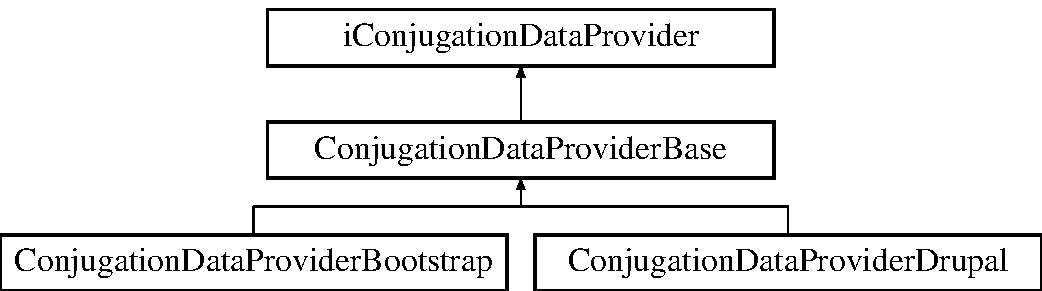
\includegraphics[height=3.000000cm]{classConjugationDataProviderBase}
\end{center}
\end{figure}
\subsection*{Fonctions membres publiques}
\begin{DoxyCompactItemize}
\item 
\hypertarget{classConjugationDataProviderBase_ad87a3d61f1cfae6a5e8e6506d1e9b57a}{}\label{classConjugationDataProviderBase_ad87a3d61f1cfae6a5e8e6506d1e9b57a} 
{\bfseries \+\_\+\+\_\+construct} (\$base\+Table\+Name)
\item 
\hyperlink{classConjugationDataProviderBase_a45ac93643d08f3099bf95faa22e9ba55}{get\+Verb} (\$verb)
\item 
\hyperlink{classConjugationDataProviderBase_a8269abd2a9be2679d2cd9f7f50ae9151}{get\+Verb\+By\+Id} (\$id)
\item 
\hyperlink{classConjugationDataProviderBase_a4be78cfcdc11584d355bdfc8b988a3ca}{get\+Verb\+Model\+Object} (\$num\+Model)
\item 
\hyperlink{classConjugationDataProviderBase_aafcbd6631477f8f634d762b5ba5dc217}{get\+Top20} ()
\item 
\hyperlink{classConjugationDataProviderBase_a964e48a9e1d9c507fdb19e96737c09e4}{get\+Others\+In\+Model} (\$verb)
\item 
\hyperlink{classConjugationDataProviderBase_a155bfe75cdc9224801c2704540205650}{get\+Count\+Others\+In\+Model} (\$verb)
\item 
\hyperlink{classConjugationDataProviderBase_a517127918e71fd89e1b7717c26353f87}{get\+Verb\+Auto\+Complete} (\$string)
\item 
\hyperlink{classConjugationDataProviderBase_aa23d566d02578adb55592bba5a796fa8}{get\+Random\+Verb} ()
\item 
\hyperlink{classConjugationDataProviderBase_a3a209dff42ff754afa7c81a8182266d7}{get\+Single\+Verbs} ()
\item 
\hyperlink{classConjugationDataProviderBase_af3d127433543eb86878447357d6382d4}{get\+All\+Verbs} ()
\item 
\hyperlink{classConjugationDataProviderBase_a645b9064803b3f6b9796fbacdb26548b}{get\+All\+Duplicated\+Verbs} ()
\item 
\hyperlink{classConjugationDataProviderBase_af619b3848a7928bc7e8f649de46e9686}{insert\+Indexed\+Verb} (array \$arr)
\item 
\hyperlink{classConjugationDataProviderBase_a12389ca76dbe2e31e08fee6b5333eed9}{get\+Verbs\+Models} ()
\item 
\hyperlink{classConjugationDataProviderBase_a779d612fb1e1d20ea7fc31511768ad66}{get\+Verbs\+Models\+Mixed} ()
\end{DoxyCompactItemize}
\subsection*{Attributs publics}
\begin{DoxyCompactItemize}
\item 
\hypertarget{classConjugationDataProviderBase_ae4dd22eb6f5454f08a9a9c3ba01e5c89}{}\label{classConjugationDataProviderBase_ae4dd22eb6f5454f08a9a9c3ba01e5c89} 
const {\bfseries I\+N\+D\+E\+X\+A\+T\+I\+O\+N\+\_\+\+S\+T\+EP} = 1000
\end{DoxyCompactItemize}
\subsection*{Fonctions membres protégées}
\begin{DoxyCompactItemize}
\item 
\hypertarget{classConjugationDataProviderBase_a3649ad489ccc588dccf840445c7432eb}{}\label{classConjugationDataProviderBase_a3649ad489ccc588dccf840445c7432eb} 
\hyperlink{classConjugationDataProviderBase_a3649ad489ccc588dccf840445c7432eb}{get\+Base\+Table\+Name} ()
\begin{DoxyCompactList}\small\item\em getter for the base\+Table\+Name which is specific for the dialect. \end{DoxyCompactList}\end{DoxyCompactItemize}
\subsection*{Attributs protégés}
\begin{DoxyCompactItemize}
\item 
\hypertarget{classConjugationDataProviderBase_ad50a1bb414ca13b00edff121abe0d0a0}{}\label{classConjugationDataProviderBase_ad50a1bb414ca13b00edff121abe0d0a0} 
{\bfseries \$\+\_\+base\+Table\+Name}
\end{DoxyCompactItemize}


\subsection{Documentation des fonctions membres}
\hypertarget{classConjugationDataProviderBase_a645b9064803b3f6b9796fbacdb26548b}{}\label{classConjugationDataProviderBase_a645b9064803b3f6b9796fbacdb26548b} 
\index{Conjugation\+Data\+Provider\+Base@{Conjugation\+Data\+Provider\+Base}!get\+All\+Duplicated\+Verbs@{get\+All\+Duplicated\+Verbs}}
\index{get\+All\+Duplicated\+Verbs@{get\+All\+Duplicated\+Verbs}!Conjugation\+Data\+Provider\+Base@{Conjugation\+Data\+Provider\+Base}}
\subsubsection{\texorpdfstring{get\+All\+Duplicated\+Verbs()}{getAllDuplicatedVerbs()}}
{\footnotesize\ttfamily Conjugation\+Data\+Provider\+Base\+::get\+All\+Duplicated\+Verbs (\begin{DoxyParamCaption}{ }\end{DoxyParamCaption})\hspace{0.3cm}{\ttfamily [abstract]}}

simple getter \hypertarget{classConjugationDataProviderBase_af3d127433543eb86878447357d6382d4}{}\label{classConjugationDataProviderBase_af3d127433543eb86878447357d6382d4} 
\index{Conjugation\+Data\+Provider\+Base@{Conjugation\+Data\+Provider\+Base}!get\+All\+Verbs@{get\+All\+Verbs}}
\index{get\+All\+Verbs@{get\+All\+Verbs}!Conjugation\+Data\+Provider\+Base@{Conjugation\+Data\+Provider\+Base}}
\subsubsection{\texorpdfstring{get\+All\+Verbs()}{getAllVerbs()}}
{\footnotesize\ttfamily Conjugation\+Data\+Provider\+Base\+::get\+All\+Verbs (\begin{DoxyParamCaption}{ }\end{DoxyParamCaption})\hspace{0.3cm}{\ttfamily [abstract]}}

simple getter \hypertarget{classConjugationDataProviderBase_a155bfe75cdc9224801c2704540205650}{}\label{classConjugationDataProviderBase_a155bfe75cdc9224801c2704540205650} 
\index{Conjugation\+Data\+Provider\+Base@{Conjugation\+Data\+Provider\+Base}!get\+Count\+Others\+In\+Model@{get\+Count\+Others\+In\+Model}}
\index{get\+Count\+Others\+In\+Model@{get\+Count\+Others\+In\+Model}!Conjugation\+Data\+Provider\+Base@{Conjugation\+Data\+Provider\+Base}}
\subsubsection{\texorpdfstring{get\+Count\+Others\+In\+Model()}{getCountOthersInModel()}}
{\footnotesize\ttfamily Conjugation\+Data\+Provider\+Base\+::get\+Count\+Others\+In\+Model (\begin{DoxyParamCaption}\item[{}]{\$verb }\end{DoxyParamCaption})\hspace{0.3cm}{\ttfamily [abstract]}}

simple getter \hypertarget{classConjugationDataProviderBase_a964e48a9e1d9c507fdb19e96737c09e4}{}\label{classConjugationDataProviderBase_a964e48a9e1d9c507fdb19e96737c09e4} 
\index{Conjugation\+Data\+Provider\+Base@{Conjugation\+Data\+Provider\+Base}!get\+Others\+In\+Model@{get\+Others\+In\+Model}}
\index{get\+Others\+In\+Model@{get\+Others\+In\+Model}!Conjugation\+Data\+Provider\+Base@{Conjugation\+Data\+Provider\+Base}}
\subsubsection{\texorpdfstring{get\+Others\+In\+Model()}{getOthersInModel()}}
{\footnotesize\ttfamily Conjugation\+Data\+Provider\+Base\+::get\+Others\+In\+Model (\begin{DoxyParamCaption}\item[{}]{\$verb }\end{DoxyParamCaption})\hspace{0.3cm}{\ttfamily [abstract]}}

simple getter \hypertarget{classConjugationDataProviderBase_aa23d566d02578adb55592bba5a796fa8}{}\label{classConjugationDataProviderBase_aa23d566d02578adb55592bba5a796fa8} 
\index{Conjugation\+Data\+Provider\+Base@{Conjugation\+Data\+Provider\+Base}!get\+Random\+Verb@{get\+Random\+Verb}}
\index{get\+Random\+Verb@{get\+Random\+Verb}!Conjugation\+Data\+Provider\+Base@{Conjugation\+Data\+Provider\+Base}}
\subsubsection{\texorpdfstring{get\+Random\+Verb()}{getRandomVerb()}}
{\footnotesize\ttfamily Conjugation\+Data\+Provider\+Base\+::get\+Random\+Verb (\begin{DoxyParamCaption}{ }\end{DoxyParamCaption})\hspace{0.3cm}{\ttfamily [abstract]}}

simple getter \hypertarget{classConjugationDataProviderBase_a3a209dff42ff754afa7c81a8182266d7}{}\label{classConjugationDataProviderBase_a3a209dff42ff754afa7c81a8182266d7} 
\index{Conjugation\+Data\+Provider\+Base@{Conjugation\+Data\+Provider\+Base}!get\+Single\+Verbs@{get\+Single\+Verbs}}
\index{get\+Single\+Verbs@{get\+Single\+Verbs}!Conjugation\+Data\+Provider\+Base@{Conjugation\+Data\+Provider\+Base}}
\subsubsection{\texorpdfstring{get\+Single\+Verbs()}{getSingleVerbs()}}
{\footnotesize\ttfamily Conjugation\+Data\+Provider\+Base\+::get\+Single\+Verbs (\begin{DoxyParamCaption}{ }\end{DoxyParamCaption})\hspace{0.3cm}{\ttfamily [abstract]}}

simple getter \hypertarget{classConjugationDataProviderBase_aafcbd6631477f8f634d762b5ba5dc217}{}\label{classConjugationDataProviderBase_aafcbd6631477f8f634d762b5ba5dc217} 
\index{Conjugation\+Data\+Provider\+Base@{Conjugation\+Data\+Provider\+Base}!get\+Top20@{get\+Top20}}
\index{get\+Top20@{get\+Top20}!Conjugation\+Data\+Provider\+Base@{Conjugation\+Data\+Provider\+Base}}
\subsubsection{\texorpdfstring{get\+Top20()}{getTop20()}}
{\footnotesize\ttfamily Conjugation\+Data\+Provider\+Base\+::get\+Top20 (\begin{DoxyParamCaption}{ }\end{DoxyParamCaption})\hspace{0.3cm}{\ttfamily [abstract]}}

simple getter \hypertarget{classConjugationDataProviderBase_a45ac93643d08f3099bf95faa22e9ba55}{}\label{classConjugationDataProviderBase_a45ac93643d08f3099bf95faa22e9ba55} 
\index{Conjugation\+Data\+Provider\+Base@{Conjugation\+Data\+Provider\+Base}!get\+Verb@{get\+Verb}}
\index{get\+Verb@{get\+Verb}!Conjugation\+Data\+Provider\+Base@{Conjugation\+Data\+Provider\+Base}}
\subsubsection{\texorpdfstring{get\+Verb()}{getVerb()}}
{\footnotesize\ttfamily Conjugation\+Data\+Provider\+Base\+::get\+Verb (\begin{DoxyParamCaption}\item[{}]{\$verb }\end{DoxyParamCaption})\hspace{0.3cm}{\ttfamily [abstract]}}

simple getter \hypertarget{classConjugationDataProviderBase_a517127918e71fd89e1b7717c26353f87}{}\label{classConjugationDataProviderBase_a517127918e71fd89e1b7717c26353f87} 
\index{Conjugation\+Data\+Provider\+Base@{Conjugation\+Data\+Provider\+Base}!get\+Verb\+Auto\+Complete@{get\+Verb\+Auto\+Complete}}
\index{get\+Verb\+Auto\+Complete@{get\+Verb\+Auto\+Complete}!Conjugation\+Data\+Provider\+Base@{Conjugation\+Data\+Provider\+Base}}
\subsubsection{\texorpdfstring{get\+Verb\+Auto\+Complete()}{getVerbAutoComplete()}}
{\footnotesize\ttfamily Conjugation\+Data\+Provider\+Base\+::get\+Verb\+Auto\+Complete (\begin{DoxyParamCaption}\item[{}]{\$string }\end{DoxyParamCaption})\hspace{0.3cm}{\ttfamily [abstract]}}

simple getter \hypertarget{classConjugationDataProviderBase_a8269abd2a9be2679d2cd9f7f50ae9151}{}\label{classConjugationDataProviderBase_a8269abd2a9be2679d2cd9f7f50ae9151} 
\index{Conjugation\+Data\+Provider\+Base@{Conjugation\+Data\+Provider\+Base}!get\+Verb\+By\+Id@{get\+Verb\+By\+Id}}
\index{get\+Verb\+By\+Id@{get\+Verb\+By\+Id}!Conjugation\+Data\+Provider\+Base@{Conjugation\+Data\+Provider\+Base}}
\subsubsection{\texorpdfstring{get\+Verb\+By\+Id()}{getVerbById()}}
{\footnotesize\ttfamily Conjugation\+Data\+Provider\+Base\+::get\+Verb\+By\+Id (\begin{DoxyParamCaption}\item[{}]{\$id }\end{DoxyParamCaption})\hspace{0.3cm}{\ttfamily [abstract]}}

simple getter \hypertarget{classConjugationDataProviderBase_a4be78cfcdc11584d355bdfc8b988a3ca}{}\label{classConjugationDataProviderBase_a4be78cfcdc11584d355bdfc8b988a3ca} 
\index{Conjugation\+Data\+Provider\+Base@{Conjugation\+Data\+Provider\+Base}!get\+Verb\+Model\+Object@{get\+Verb\+Model\+Object}}
\index{get\+Verb\+Model\+Object@{get\+Verb\+Model\+Object}!Conjugation\+Data\+Provider\+Base@{Conjugation\+Data\+Provider\+Base}}
\subsubsection{\texorpdfstring{get\+Verb\+Model\+Object()}{getVerbModelObject()}}
{\footnotesize\ttfamily Conjugation\+Data\+Provider\+Base\+::get\+Verb\+Model\+Object (\begin{DoxyParamCaption}\item[{}]{\$num\+Model }\end{DoxyParamCaption})\hspace{0.3cm}{\ttfamily [abstract]}}

simple getter \hypertarget{classConjugationDataProviderBase_a12389ca76dbe2e31e08fee6b5333eed9}{}\label{classConjugationDataProviderBase_a12389ca76dbe2e31e08fee6b5333eed9} 
\index{Conjugation\+Data\+Provider\+Base@{Conjugation\+Data\+Provider\+Base}!get\+Verbs\+Models@{get\+Verbs\+Models}}
\index{get\+Verbs\+Models@{get\+Verbs\+Models}!Conjugation\+Data\+Provider\+Base@{Conjugation\+Data\+Provider\+Base}}
\subsubsection{\texorpdfstring{get\+Verbs\+Models()}{getVerbsModels()}}
{\footnotesize\ttfamily Conjugation\+Data\+Provider\+Base\+::get\+Verbs\+Models (\begin{DoxyParamCaption}{ }\end{DoxyParamCaption})\hspace{0.3cm}{\ttfamily [abstract]}}

simple getter \hypertarget{classConjugationDataProviderBase_a779d612fb1e1d20ea7fc31511768ad66}{}\label{classConjugationDataProviderBase_a779d612fb1e1d20ea7fc31511768ad66} 
\index{Conjugation\+Data\+Provider\+Base@{Conjugation\+Data\+Provider\+Base}!get\+Verbs\+Models\+Mixed@{get\+Verbs\+Models\+Mixed}}
\index{get\+Verbs\+Models\+Mixed@{get\+Verbs\+Models\+Mixed}!Conjugation\+Data\+Provider\+Base@{Conjugation\+Data\+Provider\+Base}}
\subsubsection{\texorpdfstring{get\+Verbs\+Models\+Mixed()}{getVerbsModelsMixed()}}
{\footnotesize\ttfamily Conjugation\+Data\+Provider\+Base\+::get\+Verbs\+Models\+Mixed (\begin{DoxyParamCaption}{ }\end{DoxyParamCaption})\hspace{0.3cm}{\ttfamily [abstract]}}

simple getter \hypertarget{classConjugationDataProviderBase_af619b3848a7928bc7e8f649de46e9686}{}\label{classConjugationDataProviderBase_af619b3848a7928bc7e8f649de46e9686} 
\index{Conjugation\+Data\+Provider\+Base@{Conjugation\+Data\+Provider\+Base}!insert\+Indexed\+Verb@{insert\+Indexed\+Verb}}
\index{insert\+Indexed\+Verb@{insert\+Indexed\+Verb}!Conjugation\+Data\+Provider\+Base@{Conjugation\+Data\+Provider\+Base}}
\subsubsection{\texorpdfstring{insert\+Indexed\+Verb()}{insertIndexedVerb()}}
{\footnotesize\ttfamily Conjugation\+Data\+Provider\+Base\+::insert\+Indexed\+Verb (\begin{DoxyParamCaption}\item[{array}]{\$arr }\end{DoxyParamCaption})\hspace{0.3cm}{\ttfamily [abstract]}}

a function to update the table for indexing conjugation every time necessary 

La documentation de cette classe a été générée à partir du fichier suivant \+:\begin{DoxyCompactItemize}
\item 
php/includes/\hyperlink{ConjugationDataProviderBase_8inc}{Conjugation\+Data\+Provider\+Base.\+inc}\end{DoxyCompactItemize}

\hypertarget{classConjugationDataProviderBootstrap}{}\section{Référence de la classe Conjugation\+Data\+Provider\+Bootstrap}
\label{classConjugationDataProviderBootstrap}\index{Conjugation\+Data\+Provider\+Bootstrap@{Conjugation\+Data\+Provider\+Bootstrap}}
Graphe d\textquotesingle{}héritage de Conjugation\+Data\+Provider\+Bootstrap\+:\begin{figure}[H]
\begin{center}
\leavevmode
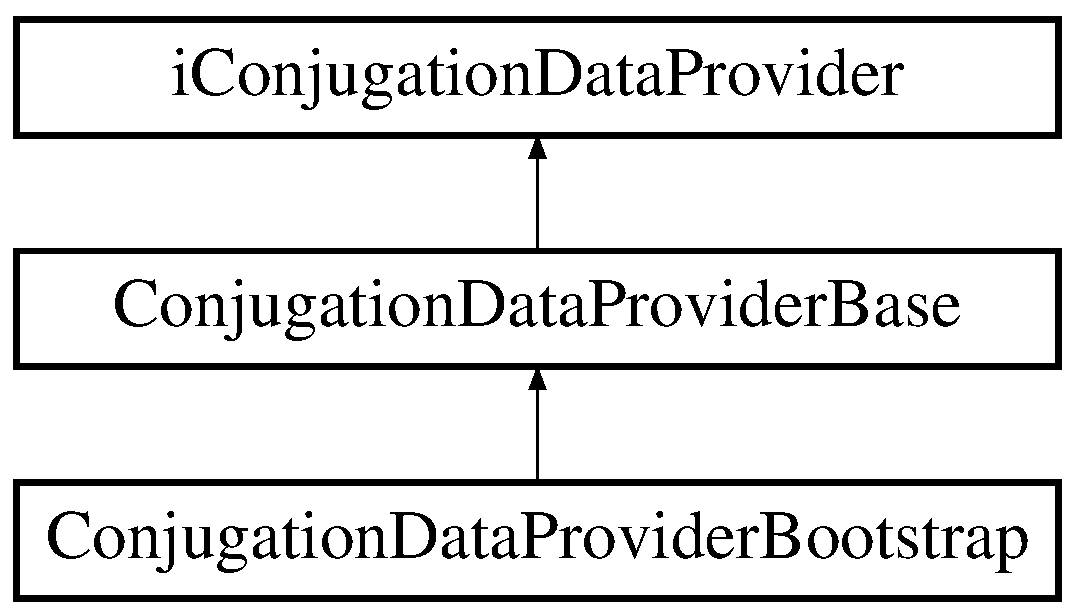
\includegraphics[height=3.000000cm]{classConjugationDataProviderBootstrap}
\end{center}
\end{figure}
\subsection*{Fonctions membres publiques}
\begin{DoxyCompactItemize}
\item 
\hypertarget{classConjugationDataProviderBootstrap_acd6426b902009eb030bafe202f23926c}{}\label{classConjugationDataProviderBootstrap_acd6426b902009eb030bafe202f23926c} 
{\bfseries \+\_\+\+\_\+construct} (\$base\+Table\+Name)
\item 
\hypertarget{classConjugationDataProviderBootstrap_a3e096bba403d060235d1ee9527c7fd6b}{}\label{classConjugationDataProviderBootstrap_a3e096bba403d060235d1ee9527c7fd6b} 
{\bfseries get\+Verb} (\$verb)
\item 
\hypertarget{classConjugationDataProviderBootstrap_ad0fde3743e27eff6e3e5249ca80018b8}{}\label{classConjugationDataProviderBootstrap_ad0fde3743e27eff6e3e5249ca80018b8} 
{\bfseries get\+Verb\+By\+Id} (\$id)
\item 
\hypertarget{classConjugationDataProviderBootstrap_aec176c34c434c97c34aec9c8b3d058cc}{}\label{classConjugationDataProviderBootstrap_aec176c34c434c97c34aec9c8b3d058cc} 
{\bfseries get\+Verb\+Model\+Object} (\$num\+Model)
\item 
\hypertarget{classConjugationDataProviderBootstrap_acd7282af2e4ac1b602656944b0459b97}{}\label{classConjugationDataProviderBootstrap_acd7282af2e4ac1b602656944b0459b97} 
{\bfseries get\+Verbs\+Models} ()
\item 
\hypertarget{classConjugationDataProviderBootstrap_a059e76472fb3972ebeeaa4060e9c22cf}{}\label{classConjugationDataProviderBootstrap_a059e76472fb3972ebeeaa4060e9c22cf} 
{\bfseries get\+Verbs\+Models\+Mixed} ()
\item 
\hypertarget{classConjugationDataProviderBootstrap_af959492587f9931545ac2290d722db5a}{}\label{classConjugationDataProviderBootstrap_af959492587f9931545ac2290d722db5a} 
{\bfseries get\+Top20} ()
\item 
\hypertarget{classConjugationDataProviderBootstrap_a26700071d61691ed0c751f061998cc81}{}\label{classConjugationDataProviderBootstrap_a26700071d61691ed0c751f061998cc81} 
{\bfseries get\+Others\+In\+Model} (\$verb)
\item 
\hypertarget{classConjugationDataProviderBootstrap_a23b3628d9f1537f4f21c46e362b4cc97}{}\label{classConjugationDataProviderBootstrap_a23b3628d9f1537f4f21c46e362b4cc97} 
{\bfseries get\+Count\+Others\+In\+Model} (\$verb)
\item 
\hypertarget{classConjugationDataProviderBootstrap_aa4a5a06e935255e64c39a0ff0584ecec}{}\label{classConjugationDataProviderBootstrap_aa4a5a06e935255e64c39a0ff0584ecec} 
{\bfseries get\+Verb\+Auto\+Complete} (\$string)
\item 
\hypertarget{classConjugationDataProviderBootstrap_a3a63ae0c2e9cb52190dced76eeaf0c20}{}\label{classConjugationDataProviderBootstrap_a3a63ae0c2e9cb52190dced76eeaf0c20} 
{\bfseries get\+Random\+Verb} ()
\item 
\hypertarget{classConjugationDataProviderBootstrap_a6ec1667942d4f6e08d5f5bf083388857}{}\label{classConjugationDataProviderBootstrap_a6ec1667942d4f6e08d5f5bf083388857} 
{\bfseries get\+Single\+Verbs} ()
\item 
\hypertarget{classConjugationDataProviderBootstrap_a3d74d3a3a754c871ac93d5a2196184b2}{}\label{classConjugationDataProviderBootstrap_a3d74d3a3a754c871ac93d5a2196184b2} 
{\bfseries get\+Verb\+F\+AR} (\$verb)
\item 
\hypertarget{classConjugationDataProviderBootstrap_a97d65e8654cbcbb6910814dc9de5a6a8}{}\label{classConjugationDataProviderBootstrap_a97d65e8654cbcbb6910814dc9de5a6a8} 
{\bfseries get\+Verb\+H\+AR} (\$verb)
\item 
\hypertarget{classConjugationDataProviderBootstrap_a5a98878c2e74fe7d3e9c53bff4250922}{}\label{classConjugationDataProviderBootstrap_a5a98878c2e74fe7d3e9c53bff4250922} 
{\bfseries get\+Indexation\+Auto\+Complete} (\$conjugation)
\item 
\hypertarget{classConjugationDataProviderBootstrap_a2e41e1de20ebc690c39f91fb05442450}{}\label{classConjugationDataProviderBootstrap_a2e41e1de20ebc690c39f91fb05442450} 
{\bfseries get\+Indexation\+Data} (\$conjugation)
\item 
\hypertarget{classConjugationDataProviderBootstrap_a0660df129657acbc695a05d6c27b4937}{}\label{classConjugationDataProviderBootstrap_a0660df129657acbc695a05d6c27b4937} 
{\bfseries get\+All\+Duplicated\+Verbs} ()
\item 
\hypertarget{classConjugationDataProviderBootstrap_a1fe64dbe28c3ed2c1c77797cb03703d8}{}\label{classConjugationDataProviderBootstrap_a1fe64dbe28c3ed2c1c77797cb03703d8} 
{\bfseries get\+All\+Verbs} ()
\item 
\hypertarget{classConjugationDataProviderBootstrap_a94516c8da8d3dd9ddbfc49ca05b355e3}{}\label{classConjugationDataProviderBootstrap_a94516c8da8d3dd9ddbfc49ca05b355e3} 
{\bfseries get\+All\+Verbs\+By\+Increment} ()
\item 
\hypertarget{classConjugationDataProviderBootstrap_a862ea39b6d38e79b84cfeaccba0fbd52}{}\label{classConjugationDataProviderBootstrap_a862ea39b6d38e79b84cfeaccba0fbd52} 
{\bfseries insert\+Indexed\+Verb} (array \$fields)
\item 
\hypertarget{classConjugationDataProviderBootstrap_a6e00cefec5c7a7821f039a263ddbe21a}{}\label{classConjugationDataProviderBootstrap_a6e00cefec5c7a7821f039a263ddbe21a} 
{\bfseries get\+Dictionary\+Definition} (\$infinitive)
\end{DoxyCompactItemize}
\subsection*{Fonctions membres protégées}
\begin{DoxyCompactItemize}
\item 
\hypertarget{classConjugationDataProviderBootstrap_a253604839693a34eb29b54e9356e40ab}{}\label{classConjugationDataProviderBootstrap_a253604839693a34eb29b54e9356e40ab} 
{\bfseries get\+Connection} ()
\end{DoxyCompactItemize}
\subsection*{Membres hérités additionnels}


La documentation de cette classe a été générée à partir du fichier suivant \+:\begin{DoxyCompactItemize}
\item 
php/includes/Conjugation\+Data\+Provider\+Bootstrap.\+inc\end{DoxyCompactItemize}

\hypertarget{classConjugationDataProviderDrupal}{}\section{Référence de la classe Conjugation\+Data\+Provider\+Drupal}
\label{classConjugationDataProviderDrupal}\index{Conjugation\+Data\+Provider\+Drupal@{Conjugation\+Data\+Provider\+Drupal}}
Graphe d\textquotesingle{}héritage de Conjugation\+Data\+Provider\+Drupal\+:\begin{figure}[H]
\begin{center}
\leavevmode
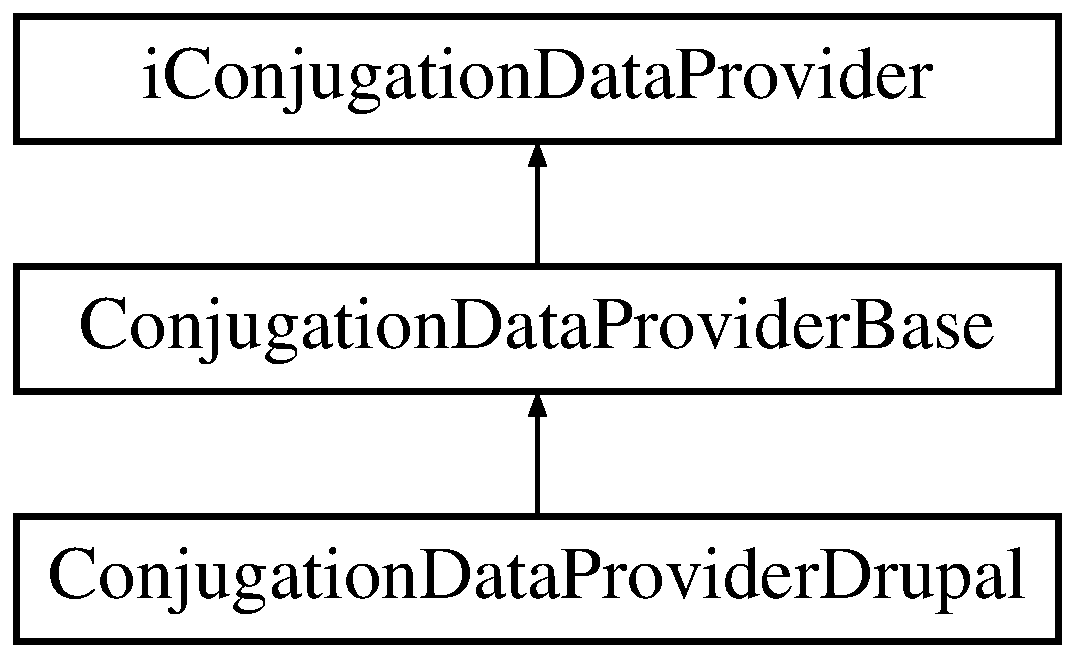
\includegraphics[height=3.000000cm]{classConjugationDataProviderDrupal}
\end{center}
\end{figure}
\subsection*{Fonctions membres publiques}
\begin{DoxyCompactItemize}
\item 
\hypertarget{classConjugationDataProviderDrupal_ade8bf964b9e3e855cdafcf620b183fe4}{}\label{classConjugationDataProviderDrupal_ade8bf964b9e3e855cdafcf620b183fe4} 
{\bfseries get\+Verb} (\$verb)
\item 
\hypertarget{classConjugationDataProviderDrupal_a1bc248d3d9e09762e4523ca230cdfdf4}{}\label{classConjugationDataProviderDrupal_a1bc248d3d9e09762e4523ca230cdfdf4} 
{\bfseries get\+Verb\+By\+Id} (\$id)
\item 
\hypertarget{classConjugationDataProviderDrupal_a2b10d06d5bab8f2315641a27aaf2f6b6}{}\label{classConjugationDataProviderDrupal_a2b10d06d5bab8f2315641a27aaf2f6b6} 
{\bfseries get\+Verb\+Model\+Object} (\$num\+Model)
\item 
\hypertarget{classConjugationDataProviderDrupal_af59dd940255f031f93d01ed07ccccbc4}{}\label{classConjugationDataProviderDrupal_af59dd940255f031f93d01ed07ccccbc4} 
{\bfseries get\+Verbs\+Models} ()
\item 
\hypertarget{classConjugationDataProviderDrupal_a03d4d222c04d356e818db0ffd86aab24}{}\label{classConjugationDataProviderDrupal_a03d4d222c04d356e818db0ffd86aab24} 
{\bfseries get\+Top20} ()
\item 
\hypertarget{classConjugationDataProviderDrupal_a2bf49d3e0b330eb944b6b64b5faf08f9}{}\label{classConjugationDataProviderDrupal_a2bf49d3e0b330eb944b6b64b5faf08f9} 
{\bfseries get\+Others\+In\+Model} (\$verb)
\item 
\hypertarget{classConjugationDataProviderDrupal_abd938073c7a5088b9a3ecd2e7ca4fb80}{}\label{classConjugationDataProviderDrupal_abd938073c7a5088b9a3ecd2e7ca4fb80} 
{\bfseries get\+Count\+Others\+In\+Model} (\$verb)
\item 
\hypertarget{classConjugationDataProviderDrupal_a52b438cebc357aac7364f344a19a3df4}{}\label{classConjugationDataProviderDrupal_a52b438cebc357aac7364f344a19a3df4} 
{\bfseries get\+Verb\+Auto\+Complete} (\$string)
\item 
\hypertarget{classConjugationDataProviderDrupal_af81203c54e0747ab8d802bf931b9efdf}{}\label{classConjugationDataProviderDrupal_af81203c54e0747ab8d802bf931b9efdf} 
{\bfseries get\+Random\+Verb} ()
\item 
\hypertarget{classConjugationDataProviderDrupal_aef3b4c81f910ce38cdb0faa3c6fee0c0}{}\label{classConjugationDataProviderDrupal_aef3b4c81f910ce38cdb0faa3c6fee0c0} 
{\bfseries get\+Single\+Verbs} ()
\item 
\hypertarget{classConjugationDataProviderDrupal_a892823740ce22d263f1cf8c9f8447f71}{}\label{classConjugationDataProviderDrupal_a892823740ce22d263f1cf8c9f8447f71} 
{\bfseries get\+Verb\+F\+AR} (\$verb)
\item 
\hypertarget{classConjugationDataProviderDrupal_ab60b9d6d1ed760ea68943419c176e997}{}\label{classConjugationDataProviderDrupal_ab60b9d6d1ed760ea68943419c176e997} 
{\bfseries get\+Verb\+H\+AR} (\$verb)
\item 
\hypertarget{classConjugationDataProviderDrupal_a9b0687eb6a86dfc120f72db8f622b3e2}{}\label{classConjugationDataProviderDrupal_a9b0687eb6a86dfc120f72db8f622b3e2} 
{\bfseries get\+Indexation\+Auto\+Complete} (\$conjugation)
\item 
\hypertarget{classConjugationDataProviderDrupal_a3cd6ea1c1628a03e31095b3c5589e9b7}{}\label{classConjugationDataProviderDrupal_a3cd6ea1c1628a03e31095b3c5589e9b7} 
{\bfseries get\+Indexation\+Data} (\$conjugation)
\item 
\hypertarget{classConjugationDataProviderDrupal_a4a933054f17ac39bc1f8511d46f458a0}{}\label{classConjugationDataProviderDrupal_a4a933054f17ac39bc1f8511d46f458a0} 
{\bfseries get\+All\+Duplicated\+Verbs} ()
\item 
\hypertarget{classConjugationDataProviderDrupal_a6f5059d90f7186ec52a2755376f2734c}{}\label{classConjugationDataProviderDrupal_a6f5059d90f7186ec52a2755376f2734c} 
{\bfseries get\+All\+Verbs} ()
\item 
\hypertarget{classConjugationDataProviderDrupal_a28b01db0d2e9a1c72f6eaadaba71de33}{}\label{classConjugationDataProviderDrupal_a28b01db0d2e9a1c72f6eaadaba71de33} 
{\bfseries get\+All\+Verbs\+By\+Increment} ()
\item 
\hypertarget{classConjugationDataProviderDrupal_a3a8340c3d8abaa7e28f2f84c8c00a307}{}\label{classConjugationDataProviderDrupal_a3a8340c3d8abaa7e28f2f84c8c00a307} 
{\bfseries insert\+Indexed\+Verb} (array \$fields)
\item 
\hypertarget{classConjugationDataProviderDrupal_ab22abe0370abb175544efd352f96a468}{}\label{classConjugationDataProviderDrupal_ab22abe0370abb175544efd352f96a468} 
{\bfseries get\+Dictionary\+Definition} (\$infinitive)
\end{DoxyCompactItemize}
\subsection*{Membres hérités additionnels}


La documentation de cette classe a été générée à partir du fichier suivant \+:\begin{DoxyCompactItemize}
\item 
php/includes/Conjugation\+Data\+Provider\+Drupal.\+inc\end{DoxyCompactItemize}

\hypertarget{classConjugationGasconAuxilliary}{}\section{Référence de la classe Conjugation\+Gascon\+Auxilliary}
\label{classConjugationGasconAuxilliary}\index{Conjugation\+Gascon\+Auxilliary@{Conjugation\+Gascon\+Auxilliary}}
Graphe d\textquotesingle{}héritage de Conjugation\+Gascon\+Auxilliary\+:\begin{figure}[H]
\begin{center}
\leavevmode
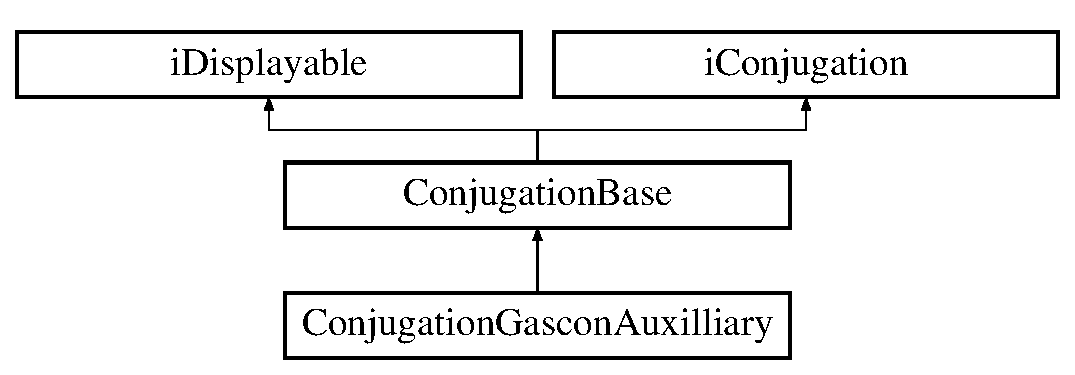
\includegraphics[height=3.000000cm]{classConjugationGasconAuxilliary}
\end{center}
\end{figure}
\subsection*{Fonctions membres publiques}
\begin{DoxyCompactItemize}
\item 
\hypertarget{classConjugationGasconAuxilliary_ace722e9b661a8c1ff4ca860682124dd4}{}\label{classConjugationGasconAuxilliary_ace722e9b661a8c1ff4ca860682124dd4} 
{\bfseries display} ()
\item 
\hypertarget{classConjugationGasconAuxilliary_ad29935aa41057e3fb1967ee425f622e2}{}\label{classConjugationGasconAuxilliary_ad29935aa41057e3fb1967ee425f622e2} 
{\bfseries get\+Conjugation\+Array} ()
\end{DoxyCompactItemize}
\subsection*{Fonctions membres protégées}
\begin{DoxyCompactItemize}
\item 
\hypertarget{classConjugationGasconAuxilliary_aee22cc89619cf7a697b30f2b2ab0eb73}{}\label{classConjugationGasconAuxilliary_aee22cc89619cf7a697b30f2b2ab0eb73} 
{\bfseries get\+Desinence\+Length\+Array} ()
\end{DoxyCompactItemize}
\subsection*{Membres hérités additionnels}


La documentation de cette classe a été générée à partir du fichier suivant \+:\begin{DoxyCompactItemize}
\item 
php/includes/Conjugation\+Gascon\+Auxilliary.\+inc\end{DoxyCompactItemize}

\hypertarget{classConjugationGasconFirstGroup}{}\section{Référence de la classe Conjugation\+Gascon\+First\+Group}
\label{classConjugationGasconFirstGroup}\index{Conjugation\+Gascon\+First\+Group@{Conjugation\+Gascon\+First\+Group}}
Graphe d\textquotesingle{}héritage de Conjugation\+Gascon\+First\+Group\+:\begin{figure}[H]
\begin{center}
\leavevmode
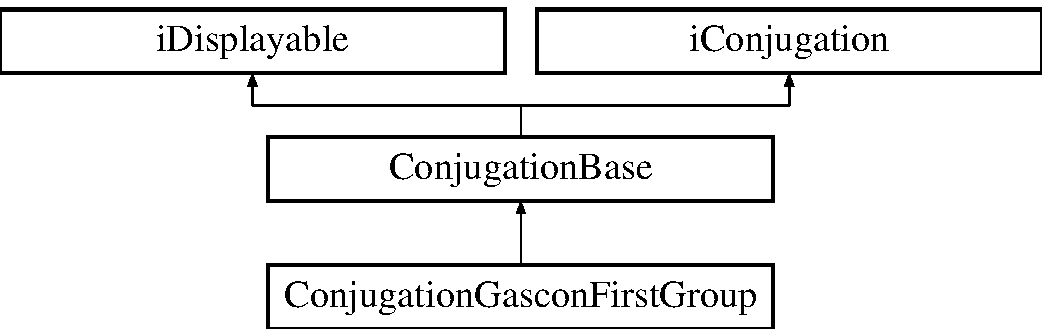
\includegraphics[height=3.000000cm]{classConjugationGasconFirstGroup}
\end{center}
\end{figure}
\subsection*{Fonctions membres publiques}
\begin{DoxyCompactItemize}
\item 
\hypertarget{classConjugationGasconFirstGroup_ace1bf96e8316a91e65e88f5e1e48c334}{}\label{classConjugationGasconFirstGroup_ace1bf96e8316a91e65e88f5e1e48c334} 
{\bfseries display} ()
\end{DoxyCompactItemize}
\subsection*{Fonctions membres protégées}
\begin{DoxyCompactItemize}
\item 
\hypertarget{classConjugationGasconFirstGroup_a60ac1ed66054150563ec6f8812861c4a}{}\label{classConjugationGasconFirstGroup_a60ac1ed66054150563ec6f8812861c4a} 
{\bfseries get\+Standard\+Conjugation} ()
\item 
\hypertarget{classConjugationGasconFirstGroup_ae03c569a6c3064a38d1eabeac9baf317}{}\label{classConjugationGasconFirstGroup_ae03c569a6c3064a38d1eabeac9baf317} 
{\bfseries fix\+Radical} (\$radical, \$desinence)
\item 
\hypertarget{classConjugationGasconFirstGroup_ad77d7a335be2cfd931aac7d90718c231}{}\label{classConjugationGasconFirstGroup_ad77d7a335be2cfd931aac7d90718c231} 
{\bfseries fix\+Desinence} (\$desinence)
\item 
\hypertarget{classConjugationGasconFirstGroup_a982308fd578abc51d30b667d5099d0c2}{}\label{classConjugationGasconFirstGroup_a982308fd578abc51d30b667d5099d0c2} 
{\bfseries get\+Conjugation\+Array} ()
\item 
\hypertarget{classConjugationGasconFirstGroup_a03a995eb9d13945f5746bf20d45c4d7f}{}\label{classConjugationGasconFirstGroup_a03a995eb9d13945f5746bf20d45c4d7f} 
{\bfseries get\+Desinence\+Length\+Array} ()
\end{DoxyCompactItemize}
\subsection*{Membres hérités additionnels}


La documentation de cette classe a été générée à partir du fichier suivant \+:\begin{DoxyCompactItemize}
\item 
php/includes/Conjugation\+Gascon\+First\+Group.\+inc\end{DoxyCompactItemize}

\hypertarget{classConjugationGasconManager}{}\section{Référence de la classe Conjugation\+Gascon\+Manager}
\label{classConjugationGasconManager}\index{Conjugation\+Gascon\+Manager@{Conjugation\+Gascon\+Manager}}
Graphe d\textquotesingle{}héritage de Conjugation\+Gascon\+Manager\+:\begin{figure}[H]
\begin{center}
\leavevmode
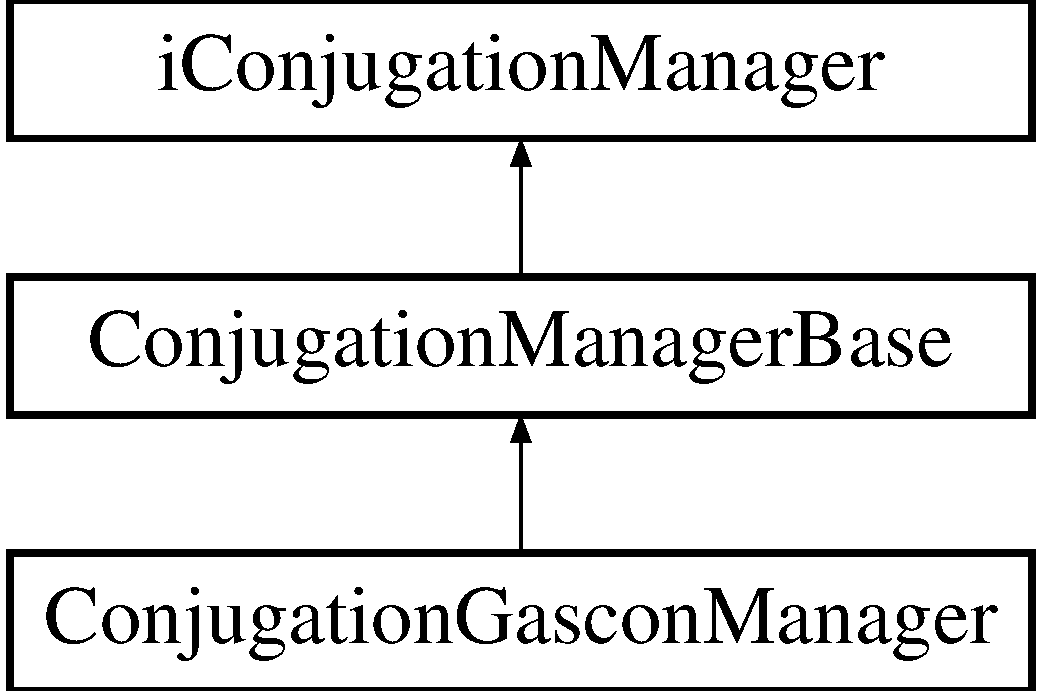
\includegraphics[height=3.000000cm]{classConjugationGasconManager}
\end{center}
\end{figure}
\subsection*{Fonctions membres publiques}
\begin{DoxyCompactItemize}
\item 
\hypertarget{classConjugationGasconManager_a2730ac29ac0ba6fd56c5896cefa297ac}{}\label{classConjugationGasconManager_a2730ac29ac0ba6fd56c5896cefa297ac} 
{\bfseries generate\+Conjugation} ()
\item 
\hyperlink{classConjugationGasconManager_a4117ecff48a5baa29d894f6174d88983}{get\+Usual\+Verbs} ()
\item 
\hypertarget{classConjugationGasconManager_a958775fb06109e0cea145f53308482b2}{}\label{classConjugationGasconManager_a958775fb06109e0cea145f53308482b2} 
{\bfseries get\+Short\+Label} ()
\item 
\hypertarget{classConjugationGasconManager_a5fc41ec1f99e255a8c57c7b7f382bc95}{}\label{classConjugationGasconManager_a5fc41ec1f99e255a8c57c7b7f382bc95} 
{\bfseries get\+Long\+Label} ()
\item 
\hypertarget{classConjugationGasconManager_a1a76a0fddebe5b28b70b532d28b0de2d}{}\label{classConjugationGasconManager_a1a76a0fddebe5b28b70b532d28b0de2d} 
{\bfseries get\+Verb\+H\+AR} (\$verb)
\end{DoxyCompactItemize}
\subsection*{Membres hérités additionnels}


\subsection{Documentation des fonctions membres}
\hypertarget{classConjugationGasconManager_a4117ecff48a5baa29d894f6174d88983}{}\label{classConjugationGasconManager_a4117ecff48a5baa29d894f6174d88983} 
\index{Conjugation\+Gascon\+Manager@{Conjugation\+Gascon\+Manager}!get\+Usual\+Verbs@{get\+Usual\+Verbs}}
\index{get\+Usual\+Verbs@{get\+Usual\+Verbs}!Conjugation\+Gascon\+Manager@{Conjugation\+Gascon\+Manager}}
\subsubsection{\texorpdfstring{get\+Usual\+Verbs()}{getUsualVerbs()}}
{\footnotesize\ttfamily Conjugation\+Gascon\+Manager\+::get\+Usual\+Verbs (\begin{DoxyParamCaption}{ }\end{DoxyParamCaption})}

\begin{DoxyReturn}{Renvoie}
an short array of verbs usually asked for. 
\end{DoxyReturn}


Implémente \hyperlink{interfaceiConjugationManager_a2a7ed39313c1c92ef5c01c88895de36e}{i\+Conjugation\+Manager}.



La documentation de cette classe a été générée à partir du fichier suivant \+:\begin{DoxyCompactItemize}
\item 
php/includes/Conjugation\+Gascon\+Manager.\+inc\end{DoxyCompactItemize}

\hypertarget{classConjugationGasconSecondGroup}{}\section{Référence de la classe Conjugation\+Gascon\+Second\+Group}
\label{classConjugationGasconSecondGroup}\index{Conjugation\+Gascon\+Second\+Group@{Conjugation\+Gascon\+Second\+Group}}
Graphe d\textquotesingle{}héritage de Conjugation\+Gascon\+Second\+Group\+:\begin{figure}[H]
\begin{center}
\leavevmode
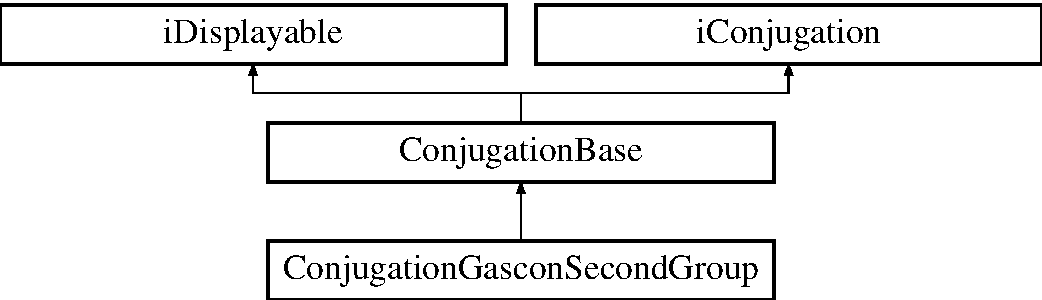
\includegraphics[height=3.000000cm]{classConjugationGasconSecondGroup}
\end{center}
\end{figure}
\subsection*{Fonctions membres publiques}
\begin{DoxyCompactItemize}
\item 
\hypertarget{classConjugationGasconSecondGroup_a6e3085b2af7792e60d3126709d8c521e}{}\label{classConjugationGasconSecondGroup_a6e3085b2af7792e60d3126709d8c521e} 
{\bfseries display} ()
\end{DoxyCompactItemize}
\subsection*{Fonctions membres protégées}
\begin{DoxyCompactItemize}
\item 
\hypertarget{classConjugationGasconSecondGroup_a53a63dc5e1a47aa4035efa26a1b45bf1}{}\label{classConjugationGasconSecondGroup_a53a63dc5e1a47aa4035efa26a1b45bf1} 
{\bfseries get\+Standard\+Conjugation} ()
\item 
\hypertarget{classConjugationGasconSecondGroup_ad51616cc8f2024140f71255e7fcc681f}{}\label{classConjugationGasconSecondGroup_ad51616cc8f2024140f71255e7fcc681f} 
{\bfseries fix\+Radical} (\$radical, \$desinence)
\item 
\hypertarget{classConjugationGasconSecondGroup_ae8d66e6a63002678daa884d3ca3a8ac1}{}\label{classConjugationGasconSecondGroup_ae8d66e6a63002678daa884d3ca3a8ac1} 
{\bfseries fix\+Desinence} (\$desinence)
\item 
\hypertarget{classConjugationGasconSecondGroup_a3702a68d3d15efe2b5109fe8800f7418}{}\label{classConjugationGasconSecondGroup_a3702a68d3d15efe2b5109fe8800f7418} 
{\bfseries get\+Conjugation\+Array} ()
\item 
\hypertarget{classConjugationGasconSecondGroup_a1584544e4c12dd19fa52703d37ced44d}{}\label{classConjugationGasconSecondGroup_a1584544e4c12dd19fa52703d37ced44d} 
{\bfseries get\+Desinence\+Length\+Array} ()
\end{DoxyCompactItemize}
\subsection*{Membres hérités additionnels}


La documentation de cette classe a été générée à partir du fichier suivant \+:\begin{DoxyCompactItemize}
\item 
php/includes/Conjugation\+Gascon\+Second\+Group.\+inc\end{DoxyCompactItemize}

\hypertarget{classConjugationGasconThirdGroup}{}\section{Référence de la classe Conjugation\+Gascon\+Third\+Group}
\label{classConjugationGasconThirdGroup}\index{Conjugation\+Gascon\+Third\+Group@{Conjugation\+Gascon\+Third\+Group}}
Graphe d\textquotesingle{}héritage de Conjugation\+Gascon\+Third\+Group\+:\begin{figure}[H]
\begin{center}
\leavevmode
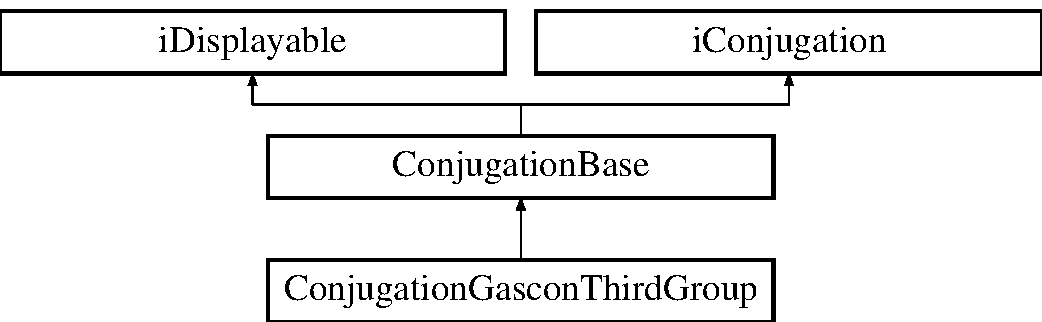
\includegraphics[height=3.000000cm]{classConjugationGasconThirdGroup}
\end{center}
\end{figure}
\subsection*{Fonctions membres publiques}
\begin{DoxyCompactItemize}
\item 
\hypertarget{classConjugationGasconThirdGroup_aded79025318b9257b1e78eb56b83408a}{}\label{classConjugationGasconThirdGroup_aded79025318b9257b1e78eb56b83408a} 
{\bfseries display} ()
\end{DoxyCompactItemize}
\subsection*{Fonctions membres protégées}
\begin{DoxyCompactItemize}
\item 
\hypertarget{classConjugationGasconThirdGroup_ae77d3521103e064d1166a896d78938cc}{}\label{classConjugationGasconThirdGroup_ae77d3521103e064d1166a896d78938cc} 
{\bfseries get\+Verbs\+Mono\+Syllabics} ()
\item 
\hypertarget{classConjugationGasconThirdGroup_a5b658699da2a8e2c53406668483816be}{}\label{classConjugationGasconThirdGroup_a5b658699da2a8e2c53406668483816be} 
{\bfseries get\+Standard\+Conjugation} ()
\item 
\hypertarget{classConjugationGasconThirdGroup_a85f7883338561152e0493cf7902cfc75}{}\label{classConjugationGasconThirdGroup_a85f7883338561152e0493cf7902cfc75} 
{\bfseries fix\+Radical} (\$radical, \$desinence)
\item 
\hypertarget{classConjugationGasconThirdGroup_a59ac06a6aa3030d98069f534ddea8398}{}\label{classConjugationGasconThirdGroup_a59ac06a6aa3030d98069f534ddea8398} 
{\bfseries fix\+Desinence} (\$desinence)
\item 
\hypertarget{classConjugationGasconThirdGroup_ab70a4b2011631eb73f3c1e20ee3fe19b}{}\label{classConjugationGasconThirdGroup_ab70a4b2011631eb73f3c1e20ee3fe19b} 
{\bfseries must\+Neutralize\+Vowel} (\$temps, \$person)
\item 
\hypertarget{classConjugationGasconThirdGroup_ab98edff3803ea21806d84b55e99b58fb}{}\label{classConjugationGasconThirdGroup_ab98edff3803ea21806d84b55e99b58fb} 
{\bfseries get\+Conjugation\+Array} ()
\item 
\hypertarget{classConjugationGasconThirdGroup_aca29f03d35cb95b12858698faf6d9a55}{}\label{classConjugationGasconThirdGroup_aca29f03d35cb95b12858698faf6d9a55} 
{\bfseries get\+Desinence\+Length\+Array} ()
\end{DoxyCompactItemize}
\subsection*{Membres hérités additionnels}


La documentation de cette classe a été générée à partir du fichier suivant \+:\begin{DoxyCompactItemize}
\item 
php/includes/Conjugation\+Gascon\+Third\+Group.\+inc\end{DoxyCompactItemize}

\hypertarget{classConjugationLengadocianAuxilliary}{}\section{Référence de la classe Conjugation\+Lengadocian\+Auxilliary}
\label{classConjugationLengadocianAuxilliary}\index{Conjugation\+Lengadocian\+Auxilliary@{Conjugation\+Lengadocian\+Auxilliary}}
Graphe d\textquotesingle{}héritage de Conjugation\+Lengadocian\+Auxilliary\+:\begin{figure}[H]
\begin{center}
\leavevmode
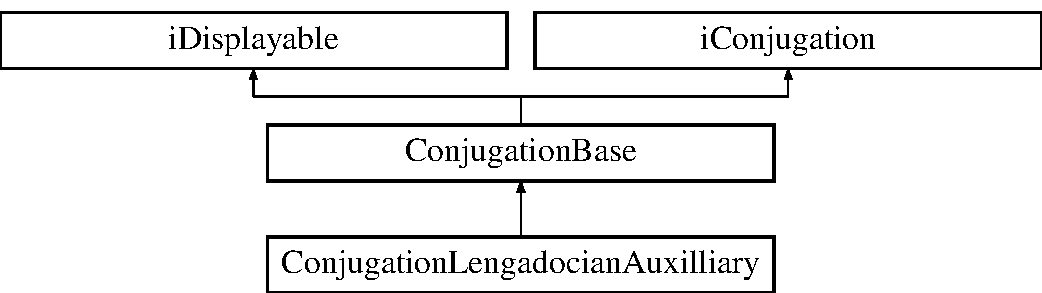
\includegraphics[height=3.000000cm]{classConjugationLengadocianAuxilliary}
\end{center}
\end{figure}
\subsection*{Fonctions membres publiques}
\begin{DoxyCompactItemize}
\item 
\hyperlink{classConjugationLengadocianAuxilliary_a4edf29f1f54605fc5876ff675827672d}{display} ()
\item 
\hyperlink{classConjugationLengadocianAuxilliary_a19fa4af3fd6382641c641a6eebb9ad68}{get\+Conjugation\+Array} ()
\end{DoxyCompactItemize}
\subsection*{Fonctions membres protégées}
\begin{DoxyCompactItemize}
\item 
\hyperlink{classConjugationLengadocianAuxilliary_a931f205d57b485b89504d879cba60230}{get\+Desinence\+Length\+Array} ()
\begin{DoxyCompactList}\small\item\em For each tempse an array entry, for each person the length of the desinence. This can vary with the model. \end{DoxyCompactList}\end{DoxyCompactItemize}
\subsection*{Membres hérités additionnels}


\subsection{Documentation des fonctions membres}
\hypertarget{classConjugationLengadocianAuxilliary_a4edf29f1f54605fc5876ff675827672d}{}\label{classConjugationLengadocianAuxilliary_a4edf29f1f54605fc5876ff675827672d} 
\index{Conjugation\+Lengadocian\+Auxilliary@{Conjugation\+Lengadocian\+Auxilliary}!display@{display}}
\index{display@{display}!Conjugation\+Lengadocian\+Auxilliary@{Conjugation\+Lengadocian\+Auxilliary}}
\subsubsection{\texorpdfstring{display()}{display()}}
{\footnotesize\ttfamily Conjugation\+Lengadocian\+Auxilliary\+::display (\begin{DoxyParamCaption}{ }\end{DoxyParamCaption})}

\begin{DoxyReturn}{Renvoie}
an empty array 
\end{DoxyReturn}


Implémente \hyperlink{interfaceiDisplayable}{i\+Displayable}.

\hypertarget{classConjugationLengadocianAuxilliary_a19fa4af3fd6382641c641a6eebb9ad68}{}\label{classConjugationLengadocianAuxilliary_a19fa4af3fd6382641c641a6eebb9ad68} 
\index{Conjugation\+Lengadocian\+Auxilliary@{Conjugation\+Lengadocian\+Auxilliary}!get\+Conjugation\+Array@{get\+Conjugation\+Array}}
\index{get\+Conjugation\+Array@{get\+Conjugation\+Array}!Conjugation\+Lengadocian\+Auxilliary@{Conjugation\+Lengadocian\+Auxilliary}}
\subsubsection{\texorpdfstring{get\+Conjugation\+Array()}{getConjugationArray()}}
{\footnotesize\ttfamily Conjugation\+Lengadocian\+Auxilliary\+::get\+Conjugation\+Array (\begin{DoxyParamCaption}{ }\end{DoxyParamCaption})}

processes the conjugation for an auxilliary and semi-\/auxilliary. There is a special treatment for the verb \char`\"{}\+F\+A\+R\char`\"{} (to do) and its production. \begin{DoxyReturn}{Renvoie}
an array 
\end{DoxyReturn}
\hypertarget{classConjugationLengadocianAuxilliary_a931f205d57b485b89504d879cba60230}{}\label{classConjugationLengadocianAuxilliary_a931f205d57b485b89504d879cba60230} 
\index{Conjugation\+Lengadocian\+Auxilliary@{Conjugation\+Lengadocian\+Auxilliary}!get\+Desinence\+Length\+Array@{get\+Desinence\+Length\+Array}}
\index{get\+Desinence\+Length\+Array@{get\+Desinence\+Length\+Array}!Conjugation\+Lengadocian\+Auxilliary@{Conjugation\+Lengadocian\+Auxilliary}}
\subsubsection{\texorpdfstring{get\+Desinence\+Length\+Array()}{getDesinenceLengthArray()}}
{\footnotesize\ttfamily Conjugation\+Lengadocian\+Auxilliary\+::get\+Desinence\+Length\+Array (\begin{DoxyParamCaption}{ }\end{DoxyParamCaption})\hspace{0.3cm}{\ttfamily [protected]}}



For each tempse an array entry, for each person the length of the desinence. This can vary with the model. 

\begin{DoxyReturn}{Renvoie}
an indexed array containing the desinence lengths. 
\end{DoxyReturn}


La documentation de cette classe a été générée à partir du fichier suivant \+:\begin{DoxyCompactItemize}
\item 
php/includes/Conjugation\+Lengadocian\+Auxilliary.\+inc\end{DoxyCompactItemize}

\hypertarget{classConjugationLengadocianFirstGroup}{}\section{Référence de la classe Conjugation\+Lengadocian\+First\+Group}
\label{classConjugationLengadocianFirstGroup}\index{Conjugation\+Lengadocian\+First\+Group@{Conjugation\+Lengadocian\+First\+Group}}
Graphe d\textquotesingle{}héritage de Conjugation\+Lengadocian\+First\+Group\+:\begin{figure}[H]
\begin{center}
\leavevmode
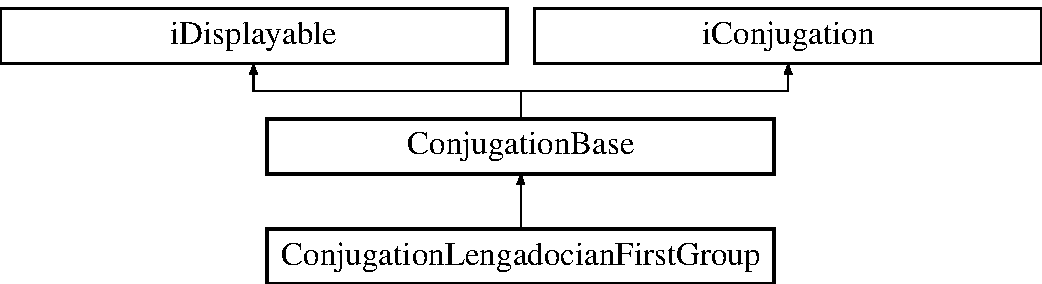
\includegraphics[height=3.000000cm]{classConjugationLengadocianFirstGroup}
\end{center}
\end{figure}
\subsection*{Fonctions membres publiques}
\begin{DoxyCompactItemize}
\item 
\hypertarget{classConjugationLengadocianFirstGroup_adca5561baef16d3a70d8ee40987bc5c0}{}\label{classConjugationLengadocianFirstGroup_adca5561baef16d3a70d8ee40987bc5c0} 
{\bfseries display} ()
\end{DoxyCompactItemize}
\subsection*{Fonctions membres protégées}
\begin{DoxyCompactItemize}
\item 
\hypertarget{classConjugationLengadocianFirstGroup_a3728df26c35bff9d1f74dd0825b30873}{}\label{classConjugationLengadocianFirstGroup_a3728df26c35bff9d1f74dd0825b30873} 
{\bfseries get\+Standard\+Conjugation} ()
\item 
\hypertarget{classConjugationLengadocianFirstGroup_ac9e14d59dc07f35e204efa14bd00d903}{}\label{classConjugationLengadocianFirstGroup_ac9e14d59dc07f35e204efa14bd00d903} 
{\bfseries fix\+Radical} (\$radical, \$desinence)
\item 
\hypertarget{classConjugationLengadocianFirstGroup_a7e9cdca67d8ed30db1ef7547c61f38da}{}\label{classConjugationLengadocianFirstGroup_a7e9cdca67d8ed30db1ef7547c61f38da} 
{\bfseries fix\+Desinence} (\$desinence)
\item 
\hypertarget{classConjugationLengadocianFirstGroup_a99becd6debfe143a6577f1ba7b063d58}{}\label{classConjugationLengadocianFirstGroup_a99becd6debfe143a6577f1ba7b063d58} 
{\bfseries get\+Conjugation\+Array} ()
\item 
\hypertarget{classConjugationLengadocianFirstGroup_a292ace5003eeb35711157918cde3c459}{}\label{classConjugationLengadocianFirstGroup_a292ace5003eeb35711157918cde3c459} 
{\bfseries get\+Desinence\+Length\+Array} ()
\end{DoxyCompactItemize}
\subsection*{Membres hérités additionnels}


La documentation de cette classe a été générée à partir du fichier suivant \+:\begin{DoxyCompactItemize}
\item 
php/includes/Conjugation\+Lengadocian\+First\+Group.\+inc\end{DoxyCompactItemize}

\hypertarget{classConjugationLengadocianManager}{}\section{Référence de la classe Conjugation\+Lengadocian\+Manager}
\label{classConjugationLengadocianManager}\index{Conjugation\+Lengadocian\+Manager@{Conjugation\+Lengadocian\+Manager}}
Graphe d\textquotesingle{}héritage de Conjugation\+Lengadocian\+Manager\+:\begin{figure}[H]
\begin{center}
\leavevmode
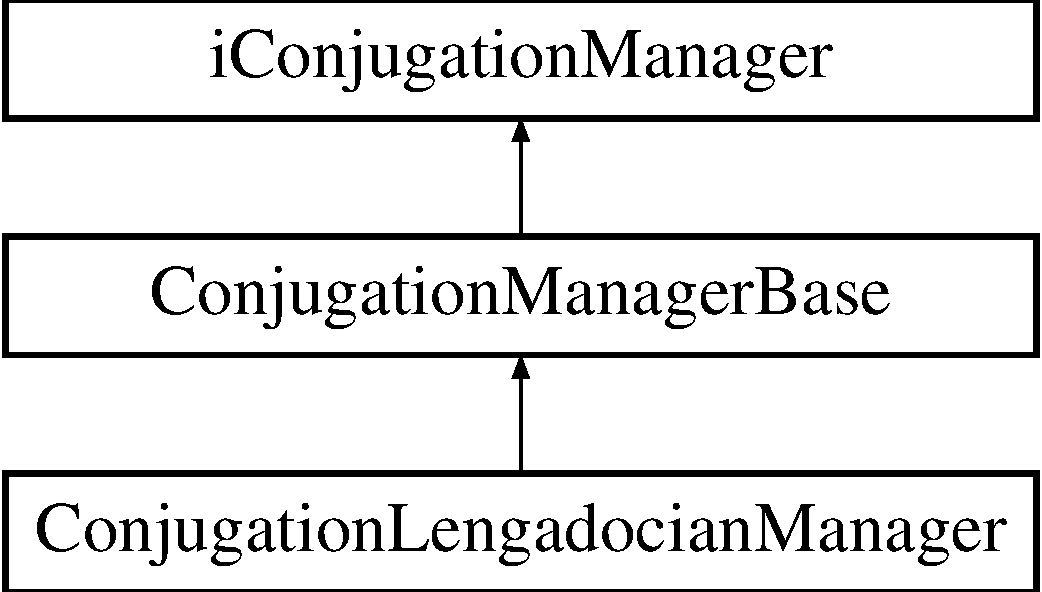
\includegraphics[height=3.000000cm]{classConjugationLengadocianManager}
\end{center}
\end{figure}
\subsection*{Fonctions membres publiques}
\begin{DoxyCompactItemize}
\item 
\hypertarget{classConjugationLengadocianManager_aaa61dfc0043e13de40d77255494cba82}{}\label{classConjugationLengadocianManager_aaa61dfc0043e13de40d77255494cba82} 
{\bfseries generate\+Conjugation} ()
\item 
\hyperlink{classConjugationLengadocianManager_a1ec18e3663eae35578b4f1967e4d981d}{get\+Usual\+Verbs} ()
\item 
\hypertarget{classConjugationLengadocianManager_a5e9c807113463d8d0044e3ba13937fa1}{}\label{classConjugationLengadocianManager_a5e9c807113463d8d0044e3ba13937fa1} 
{\bfseries get\+Verb\+F\+AR} (\$verb)
\item 
\hypertarget{classConjugationLengadocianManager_a87ad1195fe8eea002079c372843bb9fa}{}\label{classConjugationLengadocianManager_a87ad1195fe8eea002079c372843bb9fa} 
{\bfseries get\+Short\+Label} ()
\item 
\hypertarget{classConjugationLengadocianManager_ac14ff4edd45b3de2d303f2ac5fc94d91}{}\label{classConjugationLengadocianManager_ac14ff4edd45b3de2d303f2ac5fc94d91} 
{\bfseries get\+Long\+Label} ()
\end{DoxyCompactItemize}
\subsection*{Membres hérités additionnels}


\subsection{Documentation des fonctions membres}
\hypertarget{classConjugationLengadocianManager_a1ec18e3663eae35578b4f1967e4d981d}{}\label{classConjugationLengadocianManager_a1ec18e3663eae35578b4f1967e4d981d} 
\index{Conjugation\+Lengadocian\+Manager@{Conjugation\+Lengadocian\+Manager}!get\+Usual\+Verbs@{get\+Usual\+Verbs}}
\index{get\+Usual\+Verbs@{get\+Usual\+Verbs}!Conjugation\+Lengadocian\+Manager@{Conjugation\+Lengadocian\+Manager}}
\subsubsection{\texorpdfstring{get\+Usual\+Verbs()}{getUsualVerbs()}}
{\footnotesize\ttfamily Conjugation\+Lengadocian\+Manager\+::get\+Usual\+Verbs (\begin{DoxyParamCaption}{ }\end{DoxyParamCaption})}

\begin{DoxyReturn}{Renvoie}
an short array of verbs usually asked for. 
\end{DoxyReturn}


Implémente \hyperlink{interfaceiConjugationManager_a2a7ed39313c1c92ef5c01c88895de36e}{i\+Conjugation\+Manager}.



La documentation de cette classe a été générée à partir du fichier suivant \+:\begin{DoxyCompactItemize}
\item 
php/includes/Conjugation\+Lengadocian\+Manager.\+inc\end{DoxyCompactItemize}

\hypertarget{classConjugationLengadocianSecondGroup}{}\section{Référence de la classe Conjugation\+Lengadocian\+Second\+Group}
\label{classConjugationLengadocianSecondGroup}\index{Conjugation\+Lengadocian\+Second\+Group@{Conjugation\+Lengadocian\+Second\+Group}}
Graphe d\textquotesingle{}héritage de Conjugation\+Lengadocian\+Second\+Group\+:\begin{figure}[H]
\begin{center}
\leavevmode
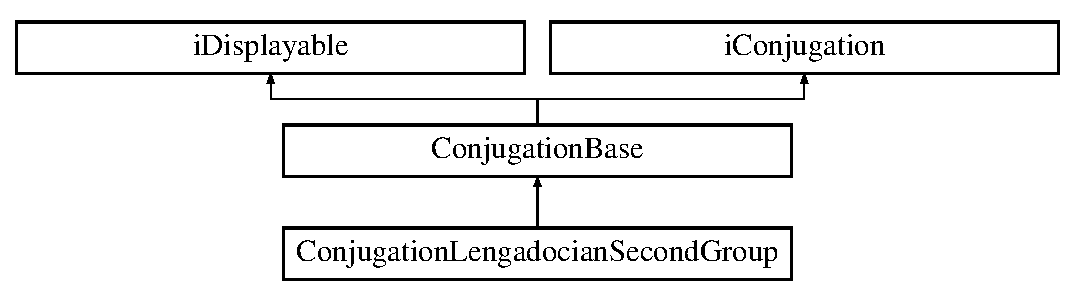
\includegraphics[height=3.000000cm]{classConjugationLengadocianSecondGroup}
\end{center}
\end{figure}
\subsection*{Fonctions membres publiques}
\begin{DoxyCompactItemize}
\item 
\hypertarget{classConjugationLengadocianSecondGroup_a9d00d6ae2616d21e1cf495ec94c06aa9}{}\label{classConjugationLengadocianSecondGroup_a9d00d6ae2616d21e1cf495ec94c06aa9} 
{\bfseries display} ()
\end{DoxyCompactItemize}
\subsection*{Fonctions membres protégées}
\begin{DoxyCompactItemize}
\item 
\hypertarget{classConjugationLengadocianSecondGroup_a710cb66b717733d6d5198e23a261bdab}{}\label{classConjugationLengadocianSecondGroup_a710cb66b717733d6d5198e23a261bdab} 
{\bfseries get\+Standard\+Conjugation} ()
\item 
\hypertarget{classConjugationLengadocianSecondGroup_a06cea5291eea31ff2aa699f5c27cbf5f}{}\label{classConjugationLengadocianSecondGroup_a06cea5291eea31ff2aa699f5c27cbf5f} 
{\bfseries get\+Conjugation\+Array} ()
\item 
\hypertarget{classConjugationLengadocianSecondGroup_a8230cbb2d79d7ce6d85b866082925b12}{}\label{classConjugationLengadocianSecondGroup_a8230cbb2d79d7ce6d85b866082925b12} 
{\bfseries get\+Desinence\+Length\+Array} ()
\item 
\hypertarget{classConjugationLengadocianSecondGroup_a236aaf5140e4cb5738a2af876eded810}{}\label{classConjugationLengadocianSecondGroup_a236aaf5140e4cb5738a2af876eded810} 
{\bfseries fix\+Radical} (\$radical, \$desinence)
\end{DoxyCompactItemize}
\subsection*{Membres hérités additionnels}


La documentation de cette classe a été générée à partir du fichier suivant \+:\begin{DoxyCompactItemize}
\item 
php/includes/Conjugation\+Lengadocian\+Second\+Group.\+inc\end{DoxyCompactItemize}

\hypertarget{classConjugationLengadocianThirdGroup}{}\section{Référence de la classe Conjugation\+Lengadocian\+Third\+Group}
\label{classConjugationLengadocianThirdGroup}\index{Conjugation\+Lengadocian\+Third\+Group@{Conjugation\+Lengadocian\+Third\+Group}}
Graphe d\textquotesingle{}héritage de Conjugation\+Lengadocian\+Third\+Group\+:\begin{figure}[H]
\begin{center}
\leavevmode
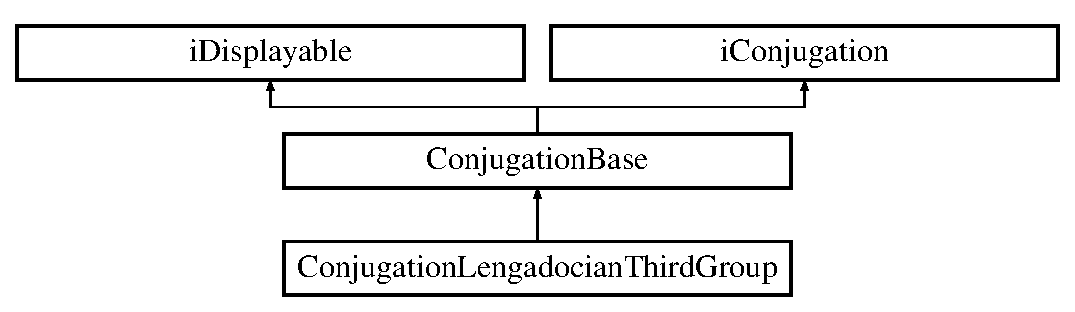
\includegraphics[height=3.000000cm]{classConjugationLengadocianThirdGroup}
\end{center}
\end{figure}
\subsection*{Fonctions membres publiques}
\begin{DoxyCompactItemize}
\item 
\hypertarget{classConjugationLengadocianThirdGroup_a13c6997dad7cbe8c53fe4ecbad7367ab}{}\label{classConjugationLengadocianThirdGroup_a13c6997dad7cbe8c53fe4ecbad7367ab} 
{\bfseries display} ()
\end{DoxyCompactItemize}
\subsection*{Fonctions membres protégées}
\begin{DoxyCompactItemize}
\item 
\hypertarget{classConjugationLengadocianThirdGroup_a74123f02b8ac3ab7730bbc935acaefd5}{}\label{classConjugationLengadocianThirdGroup_a74123f02b8ac3ab7730bbc935acaefd5} 
{\bfseries get\+Standard\+Conjugation} ()
\item 
\hypertarget{classConjugationLengadocianThirdGroup_a11aedf41cff74c08a1bfd25ac5ce8709}{}\label{classConjugationLengadocianThirdGroup_a11aedf41cff74c08a1bfd25ac5ce8709} 
{\bfseries get\+Conjugation\+Array} ()
\item 
\hypertarget{classConjugationLengadocianThirdGroup_a24ef94ab2752b9ab2eadbefda6ddd959}{}\label{classConjugationLengadocianThirdGroup_a24ef94ab2752b9ab2eadbefda6ddd959} 
{\bfseries fix\+Radical} (\$radical, \$desinence)
\item 
\hypertarget{classConjugationLengadocianThirdGroup_a6c1f315bacb649a252e5058a28f46141}{}\label{classConjugationLengadocianThirdGroup_a6c1f315bacb649a252e5058a28f46141} 
{\bfseries fix\+Desinence} (\$desinence)
\item 
\hypertarget{classConjugationLengadocianThirdGroup_a728d85569c753bf2a42e963e51aeadfa}{}\label{classConjugationLengadocianThirdGroup_a728d85569c753bf2a42e963e51aeadfa} 
{\bfseries get\+Desinence\+Length\+Array} ()
\end{DoxyCompactItemize}
\subsection*{Membres hérités additionnels}


La documentation de cette classe a été générée à partir du fichier suivant \+:\begin{DoxyCompactItemize}
\item 
php/includes/Conjugation\+Lengadocian\+Third\+Group.\+inc\end{DoxyCompactItemize}

\hypertarget{classConjugationManagerBase}{}\section{Référence de la classe Conjugation\+Manager\+Base}
\label{classConjugationManagerBase}\index{Conjugation\+Manager\+Base@{Conjugation\+Manager\+Base}}
Graphe d\textquotesingle{}héritage de Conjugation\+Manager\+Base\+:\begin{figure}[H]
\begin{center}
\leavevmode
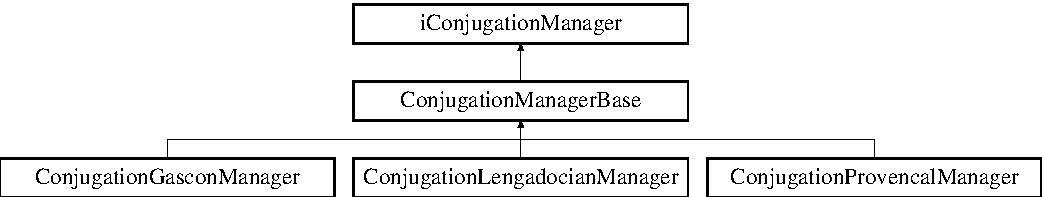
\includegraphics[height=2.654028cm]{classConjugationManagerBase}
\end{center}
\end{figure}
\subsection*{Fonctions membres publiques}
\begin{DoxyCompactItemize}
\item 
\hypertarget{classConjugationManagerBase_a50aa5bd320294aa9683a54dc1b51273f}{}\label{classConjugationManagerBase_a50aa5bd320294aa9683a54dc1b51273f} 
{\bfseries get\+Dialect} ()
\item 
\hypertarget{classConjugationManagerBase_a4f3830c6823fd2add6dc25a69a0e507c}{}\label{classConjugationManagerBase_a4f3830c6823fd2add6dc25a69a0e507c} 
{\bfseries get\+Dialect\+Code} ()
\item 
\hyperlink{classConjugationManagerBase_a266802b93062d79fa75c460dc72945d8}{set\+Dialect} (\$dialect)
\item 
\hyperlink{classConjugationManagerBase_a98c6196247fa40cca8701324bdf36897}{set\+Dialect\+Code} (\$dialect\+Code)
\begin{DoxyCompactList}\small\item\em a setter \end{DoxyCompactList}\item 
\hyperlink{classConjugationManagerBase_ae6e9d7d21418b8b9831b2b1f29eca4a6}{get\+Verb} ()
\begin{DoxyCompactList}\small\item\em a getter \end{DoxyCompactList}\item 
\hyperlink{classConjugationManagerBase_a36a53a9f0bc2114a5429bcf9e3cd351e}{set\+Verb} (\$verb)
\begin{DoxyCompactList}\small\item\em more than a setter the dataprovider gets all the information for the verb if the verb is not found the object is filled w/ null values \end{DoxyCompactList}\item 
\hypertarget{classConjugationManagerBase_aecf22ced680433bb1c366d0de3931bac}{}\label{classConjugationManagerBase_aecf22ced680433bb1c366d0de3931bac} 
{\bfseries get\+Verb\+Model} ()
\item 
\hypertarget{classConjugationManagerBase_a7169d09d7207a9ca1ad4cda9a319effd}{}\label{classConjugationManagerBase_a7169d09d7207a9ca1ad4cda9a319effd} 
{\bfseries get\+Verb\+Model\+Object} (\$nummodel)
\item 
\hypertarget{classConjugationManagerBase_a3fca72bd4f7e23d7c7e5a4b3b209387b}{}\label{classConjugationManagerBase_a3fca72bd4f7e23d7c7e5a4b3b209387b} 
{\bfseries get\+Group} ()
\item 
\hypertarget{classConjugationManagerBase_a33531e6e7b32ecb2514431628fae41cf}{}\label{classConjugationManagerBase_a33531e6e7b32ecb2514431628fae41cf} 
{\bfseries get\+See\+Also} ()
\item 
\hypertarget{classConjugationManagerBase_ae737f3f0ee24fc29c25460391bd66ac1}{}\label{classConjugationManagerBase_ae737f3f0ee24fc29c25460391bd66ac1} 
{\bfseries get\+Alias} ()
\item 
\hypertarget{classConjugationManagerBase_a840c42ab40fd243dc6fc60f977919c39}{}\label{classConjugationManagerBase_a840c42ab40fd243dc6fc60f977919c39} 
{\bfseries get\+Verb\+Id} ()
\item 
\hypertarget{classConjugationManagerBase_aa6fcffaba728e6eb5b28503066bd4b0f}{}\label{classConjugationManagerBase_aa6fcffaba728e6eb5b28503066bd4b0f} 
{\bfseries get\+Comments} ()
\item 
\hypertarget{classConjugationManagerBase_a408ff3238b71c5e124eb4226a6a92792}{}\label{classConjugationManagerBase_a408ff3238b71c5e124eb4226a6a92792} 
{\bfseries get\+Lib\+Model} ()
\item 
\hypertarget{classConjugationManagerBase_a4c0cb7963519040f87daf34541f9ddb9}{}\label{classConjugationManagerBase_a4c0cb7963519040f87daf34541f9ddb9} 
{\bfseries get\+Localization} ()
\item 
\hypertarget{classConjugationManagerBase_acc0444052a240e9b9afabc6f045f9062}{}\label{classConjugationManagerBase_acc0444052a240e9b9afabc6f045f9062} 
{\bfseries get\+Conjugations} ()
\item 
\hypertarget{classConjugationManagerBase_a00fa131c934b5e69b396090dc393215d}{}\label{classConjugationManagerBase_a00fa131c934b5e69b396090dc393215d} 
{\bfseries get\+Dictionary\+Definition} (\$infinitive)
\item 
\hypertarget{classConjugationManagerBase_a6ac46ba320536e11f2f0eedb2e04fced}{}\label{classConjugationManagerBase_a6ac46ba320536e11f2f0eedb2e04fced} 
{\bfseries get\+Row} ()
\item 
\hypertarget{classConjugationManagerBase_a1d66b72e31e4eff2263a15837e7a7c7d}{}\label{classConjugationManagerBase_a1d66b72e31e4eff2263a15837e7a7c7d} 
{\bfseries get\+Provider} ()
\item 
\hyperlink{classConjugationManagerBase_a63728ecfb3a2eb259accf59dd79e9c26}{get\+Top20} ()
\item 
\hypertarget{classConjugationManagerBase_ac463846b6db0ebc24dbcc8ee08cf0fae}{}\label{classConjugationManagerBase_ac463846b6db0ebc24dbcc8ee08cf0fae} 
{\bfseries get\+Others\+In\+Model} (\$verb)
\item 
\hypertarget{classConjugationManagerBase_a170ee674be3f030087e4e77489623e4a}{}\label{classConjugationManagerBase_a170ee674be3f030087e4e77489623e4a} 
{\bfseries get\+Count\+Others\+In\+Model} (\$verb)
\item 
\hypertarget{classConjugationManagerBase_adaa1d873ae00ca4cd2dcba8bac138b88}{}\label{classConjugationManagerBase_adaa1d873ae00ca4cd2dcba8bac138b88} 
{\bfseries get\+Single\+Verbs} ()
\item 
\hypertarget{classConjugationManagerBase_ac645c98d094ad5be6eec9950d04ee937}{}\label{classConjugationManagerBase_ac645c98d094ad5be6eec9950d04ee937} 
{\bfseries get\+Verb\+Auto\+Complete} (\$string)
\item 
\hypertarget{classConjugationManagerBase_a8686180500ee969d111c7764d52a1725}{}\label{classConjugationManagerBase_a8686180500ee969d111c7764d52a1725} 
{\bfseries get\+Indexation\+Auto\+Complete} (\$string)
\item 
\hypertarget{classConjugationManagerBase_a51e5b1141591ac39b9b92a46411b688c}{}\label{classConjugationManagerBase_a51e5b1141591ac39b9b92a46411b688c} 
{\bfseries get\+Indexation\+Data} (\$conjugation)
\item 
\hyperlink{classConjugationManagerBase_ac2e82ace9b19d7b014908ec275b552bc}{get\+Random\+Verb} ()
\item 
\hyperlink{classConjugationManagerBase_a1dff05e951fe4453247a97f5aff5bc83}{get\+Usual\+Verbs} ()
\item 
\hypertarget{classConjugationManagerBase_aa4e4c35d0affaf806ee807878a507b3e}{}\label{classConjugationManagerBase_aa4e4c35d0affaf806ee807878a507b3e} 
{\bfseries generate\+Conjugation} ()
\item 
\hyperlink{classConjugationManagerBase_a20e28aa17935e10b1a763b39a3c4fdf3}{conjugate} ()
\begin{DoxyCompactList}\small\item\em immediatly called after setting a verb. \end{DoxyCompactList}\item 
\hypertarget{classConjugationManagerBase_ad8091fd5ac8eb3c036de220ec6932234}{}\label{classConjugationManagerBase_ad8091fd5ac8eb3c036de220ec6932234} 
{\bfseries process\+Indexation\+Once} (\$arr\+Verb)
\item 
\hypertarget{classConjugationManagerBase_aa8df6ff754ed94b8771aebff95e6e3fe}{}\label{classConjugationManagerBase_aa8df6ff754ed94b8771aebff95e6e3fe} 
{\bfseries process\+Indexation} ()
\item 
\hypertarget{classConjugationManagerBase_ababdfdc7a62b48362bcdfa38aed647d5}{}\label{classConjugationManagerBase_ababdfdc7a62b48362bcdfa38aed647d5} 
{\bfseries get\+Short\+Label} ()
\item 
\hypertarget{classConjugationManagerBase_adc1333ad8b45b63d63424c2b6754e8f5}{}\label{classConjugationManagerBase_adc1333ad8b45b63d63424c2b6754e8f5} 
{\bfseries get\+Long\+Label} ()
\item 
\hypertarget{classConjugationManagerBase_ac7e4846ef7b60545bb2b4d77f6bf7f0f}{}\label{classConjugationManagerBase_ac7e4846ef7b60545bb2b4d77f6bf7f0f} 
{\bfseries get\+Verbs\+Models} ()
\item 
\hypertarget{classConjugationManagerBase_a87ceb2a9767830108d01928c19a90f83}{}\label{classConjugationManagerBase_a87ceb2a9767830108d01928c19a90f83} 
{\bfseries get\+Verbs\+Models\+Mixed} ()
\end{DoxyCompactItemize}
\subsection*{Fonctions membres publiques statiques}
\begin{DoxyCompactItemize}
\item 
\hypertarget{classConjugationManagerBase_a0249bf3a9b7eb739e074bac74c436cdc}{}\label{classConjugationManagerBase_a0249bf3a9b7eb739e074bac74c436cdc} 
static {\bfseries get\+This\+Dialect\+Code} (\$dialect)
\end{DoxyCompactItemize}
\subsection*{Attributs publics}
\begin{DoxyCompactItemize}
\item 
const \hyperlink{classConjugationManagerBase_aa525010174d498dcf8d808cd3260ec02}{L\+E\+N\+G\+A\+D\+O\+C\+I\+AN} = \char`\"{}lengadocian\char`\"{}
\item 
\hypertarget{classConjugationManagerBase_ab9472d32ede192022beef2300600bc63}{}\label{classConjugationManagerBase_ab9472d32ede192022beef2300600bc63} 
const {\bfseries G\+A\+S\+C\+ON} = \char`\"{}gascon\char`\"{}
\item 
\hypertarget{classConjugationManagerBase_aafca1739a737b1e773d6b0d9a06a550f}{}\label{classConjugationManagerBase_aafca1739a737b1e773d6b0d9a06a550f} 
const {\bfseries P\+R\+O\+V\+E\+N\+C\+AL} = \char`\"{}provencal\char`\"{}
\item 
\hypertarget{classConjugationManagerBase_af9c28ee0bf06bbf9817d3fc45fc0cc9f}{}\label{classConjugationManagerBase_af9c28ee0bf06bbf9817d3fc45fc0cc9f} 
const {\bfseries V\+I\+V\+A\+R\+O\+A\+L\+P\+E\+NC} = \char`\"{}vivaro-\/alpenc\char`\"{}
\item 
\hypertarget{classConjugationManagerBase_ad7b0a080735256224a1bb452ba945075}{}\label{classConjugationManagerBase_ad7b0a080735256224a1bb452ba945075} 
const {\bfseries A\+U\+V\+E\+R\+N\+H\+AT} = \char`\"{}auvernhat\char`\"{}
\item 
\hypertarget{classConjugationManagerBase_af5089c053a0abbb1d3c9ec9101f51523}{}\label{classConjugationManagerBase_af5089c053a0abbb1d3c9ec9101f51523} 
const {\bfseries L\+E\+M\+O\+S\+IN} = \char`\"{}lemosin\char`\"{}
\item 
\hypertarget{classConjugationManagerBase_a4553efa71470b7eeed6ee2990c401b79}{}\label{classConjugationManagerBase_a4553efa71470b7eeed6ee2990c401b79} 
const {\bfseries L\+E\+N\+G\+A\+D\+O\+C\+I\+A\+N\+\_\+\+C\+O\+DE} = \char`\"{}lng\char`\"{}
\item 
\hypertarget{classConjugationManagerBase_aa94d935cbf435467c8cfaec38d6a6726}{}\label{classConjugationManagerBase_aa94d935cbf435467c8cfaec38d6a6726} 
const {\bfseries G\+A\+S\+C\+O\+N\+\_\+\+C\+O\+DE} = \char`\"{}gsc\char`\"{}
\item 
\hypertarget{classConjugationManagerBase_a9dfc042d349e57819659d964c2870135}{}\label{classConjugationManagerBase_a9dfc042d349e57819659d964c2870135} 
const {\bfseries P\+R\+O\+V\+E\+N\+C\+A\+L\+\_\+\+C\+O\+DE} = \char`\"{}prv\char`\"{}
\item 
\hypertarget{classConjugationManagerBase_a73f34b8b178aa35bcc8d35515e44d306}{}\label{classConjugationManagerBase_a73f34b8b178aa35bcc8d35515e44d306} 
const {\bfseries V\+I\+V\+A\+R\+O\+A\+L\+P\+E\+N\+C\+\_\+\+C\+O\+DE} = \char`\"{}alp\char`\"{}
\item 
\hypertarget{classConjugationManagerBase_ac915776393fb88313fc9594acabc5c0e}{}\label{classConjugationManagerBase_ac915776393fb88313fc9594acabc5c0e} 
const {\bfseries A\+U\+V\+E\+R\+N\+H\+A\+T\+\_\+\+C\+O\+DE} = \char`\"{}auv\char`\"{}
\item 
\hypertarget{classConjugationManagerBase_ab0a3fa2a7d3193603810cf5bed0a43b4}{}\label{classConjugationManagerBase_ab0a3fa2a7d3193603810cf5bed0a43b4} 
const {\bfseries L\+E\+M\+O\+S\+I\+N\+\_\+\+C\+O\+DE} = \char`\"{}lem\char`\"{}
\item 
\hypertarget{classConjugationManagerBase_acccc3a065b6c4c237da9519ee533e698}{}\label{classConjugationManagerBase_acccc3a065b6c4c237da9519ee533e698} 
const {\bfseries M\+A\+X\+\_\+\+O\+T\+H\+E\+R\+V\+E\+R\+BS} = 50
\end{DoxyCompactItemize}
\subsection*{Attributs protégés}
\begin{DoxyCompactItemize}
\item 
\hypertarget{classConjugationManagerBase_a9c3e02fa3b9610f261885b032164d81b}{}\label{classConjugationManagerBase_a9c3e02fa3b9610f261885b032164d81b} 
{\bfseries \$\+\_\+base\+Tablename}
\end{DoxyCompactItemize}


\subsection{Documentation des fonctions membres}
\hypertarget{classConjugationManagerBase_a20e28aa17935e10b1a763b39a3c4fdf3}{}\label{classConjugationManagerBase_a20e28aa17935e10b1a763b39a3c4fdf3} 
\index{Conjugation\+Manager\+Base@{Conjugation\+Manager\+Base}!conjugate@{conjugate}}
\index{conjugate@{conjugate}!Conjugation\+Manager\+Base@{Conjugation\+Manager\+Base}}
\subsubsection{\texorpdfstring{conjugate()}{conjugate()}}
{\footnotesize\ttfamily Conjugation\+Manager\+Base\+::conjugate (\begin{DoxyParamCaption}{ }\end{DoxyParamCaption})}



immediatly called after setting a verb. 

\begin{DoxySeeAlso}{Voir également}
\hyperlink{classConjugationManagerBase_a36a53a9f0bc2114a5429bcf9e3cd351e}{set\+Verb}(\$verb) 
\end{DoxySeeAlso}
\begin{DoxyReturn}{Renvoie}
a Conjugation object of an already set verb. 
\end{DoxyReturn}


Implémente \hyperlink{interfaceiConjugationManager_afba24324d7c48d3ab00ffba63cbc1b9e}{i\+Conjugation\+Manager}.

\hypertarget{classConjugationManagerBase_ac2e82ace9b19d7b014908ec275b552bc}{}\label{classConjugationManagerBase_ac2e82ace9b19d7b014908ec275b552bc} 
\index{Conjugation\+Manager\+Base@{Conjugation\+Manager\+Base}!get\+Random\+Verb@{get\+Random\+Verb}}
\index{get\+Random\+Verb@{get\+Random\+Verb}!Conjugation\+Manager\+Base@{Conjugation\+Manager\+Base}}
\subsubsection{\texorpdfstring{get\+Random\+Verb()}{getRandomVerb()}}
{\footnotesize\ttfamily Conjugation\+Manager\+Base\+::get\+Random\+Verb (\begin{DoxyParamCaption}{ }\end{DoxyParamCaption})}

\begin{DoxyReturn}{Renvoie}
a string, a verb at random in its infinitive mood. 
\end{DoxyReturn}


Implémente \hyperlink{interfaceiConjugationManager_a2e955e8c88d45869683005343cbfac60}{i\+Conjugation\+Manager}.

\hypertarget{classConjugationManagerBase_a63728ecfb3a2eb259accf59dd79e9c26}{}\label{classConjugationManagerBase_a63728ecfb3a2eb259accf59dd79e9c26} 
\index{Conjugation\+Manager\+Base@{Conjugation\+Manager\+Base}!get\+Top20@{get\+Top20}}
\index{get\+Top20@{get\+Top20}!Conjugation\+Manager\+Base@{Conjugation\+Manager\+Base}}
\subsubsection{\texorpdfstring{get\+Top20()}{getTop20()}}
{\footnotesize\ttfamily Conjugation\+Manager\+Base\+::get\+Top20 (\begin{DoxyParamCaption}{ }\end{DoxyParamCaption})}

\begin{DoxyReturn}{Renvoie}
an array of 20 of the most asked verbs 
\end{DoxyReturn}


Implémente \hyperlink{interfaceiConjugationManager_a0273fc00cbbf9e83823d571e3e2c8945}{i\+Conjugation\+Manager}.

\hypertarget{classConjugationManagerBase_a1dff05e951fe4453247a97f5aff5bc83}{}\label{classConjugationManagerBase_a1dff05e951fe4453247a97f5aff5bc83} 
\index{Conjugation\+Manager\+Base@{Conjugation\+Manager\+Base}!get\+Usual\+Verbs@{get\+Usual\+Verbs}}
\index{get\+Usual\+Verbs@{get\+Usual\+Verbs}!Conjugation\+Manager\+Base@{Conjugation\+Manager\+Base}}
\subsubsection{\texorpdfstring{get\+Usual\+Verbs()}{getUsualVerbs()}}
{\footnotesize\ttfamily Conjugation\+Manager\+Base\+::get\+Usual\+Verbs (\begin{DoxyParamCaption}{ }\end{DoxyParamCaption})\hspace{0.3cm}{\ttfamily [abstract]}}

\begin{DoxyReturn}{Renvoie}
an short array of verbs usually asked for. 
\end{DoxyReturn}


Implémente \hyperlink{interfaceiConjugationManager_a2a7ed39313c1c92ef5c01c88895de36e}{i\+Conjugation\+Manager}.

\hypertarget{classConjugationManagerBase_ae6e9d7d21418b8b9831b2b1f29eca4a6}{}\label{classConjugationManagerBase_ae6e9d7d21418b8b9831b2b1f29eca4a6} 
\index{Conjugation\+Manager\+Base@{Conjugation\+Manager\+Base}!get\+Verb@{get\+Verb}}
\index{get\+Verb@{get\+Verb}!Conjugation\+Manager\+Base@{Conjugation\+Manager\+Base}}
\subsubsection{\texorpdfstring{get\+Verb()}{getVerb()}}
{\footnotesize\ttfamily Conjugation\+Manager\+Base\+::get\+Verb (\begin{DoxyParamCaption}{ }\end{DoxyParamCaption})}



a getter 

\begin{DoxyReturn}{Renvoie}
the infinitve mood of the verb 
\end{DoxyReturn}
\hypertarget{classConjugationManagerBase_a266802b93062d79fa75c460dc72945d8}{}\label{classConjugationManagerBase_a266802b93062d79fa75c460dc72945d8} 
\index{Conjugation\+Manager\+Base@{Conjugation\+Manager\+Base}!set\+Dialect@{set\+Dialect}}
\index{set\+Dialect@{set\+Dialect}!Conjugation\+Manager\+Base@{Conjugation\+Manager\+Base}}
\subsubsection{\texorpdfstring{set\+Dialect()}{setDialect()}}
{\footnotesize\ttfamily Conjugation\+Manager\+Base\+::set\+Dialect (\begin{DoxyParamCaption}\item[{}]{\$dialect }\end{DoxyParamCaption})}


\begin{DoxyParams}{Paramètres}
{\em \$dialect} & a string to set the name of the tables in the database for this very dialect. \\
\hline
\end{DoxyParams}
\begin{DoxySeeAlso}{Voir également}
i\+Conjugation\+Data\+Provider 
\end{DoxySeeAlso}
\hypertarget{classConjugationManagerBase_a98c6196247fa40cca8701324bdf36897}{}\label{classConjugationManagerBase_a98c6196247fa40cca8701324bdf36897} 
\index{Conjugation\+Manager\+Base@{Conjugation\+Manager\+Base}!set\+Dialect\+Code@{set\+Dialect\+Code}}
\index{set\+Dialect\+Code@{set\+Dialect\+Code}!Conjugation\+Manager\+Base@{Conjugation\+Manager\+Base}}
\subsubsection{\texorpdfstring{set\+Dialect\+Code()}{setDialectCode()}}
{\footnotesize\ttfamily Conjugation\+Manager\+Base\+::set\+Dialect\+Code (\begin{DoxyParamCaption}\item[{}]{\$dialect\+Code }\end{DoxyParamCaption})}



a setter 


\begin{DoxyParams}{Paramètres}
{\em \$dialect\+Code} & a string to set the name of the tables in the database for this very dialect. \\
\hline
\end{DoxyParams}
\hypertarget{classConjugationManagerBase_a36a53a9f0bc2114a5429bcf9e3cd351e}{}\label{classConjugationManagerBase_a36a53a9f0bc2114a5429bcf9e3cd351e} 
\index{Conjugation\+Manager\+Base@{Conjugation\+Manager\+Base}!set\+Verb@{set\+Verb}}
\index{set\+Verb@{set\+Verb}!Conjugation\+Manager\+Base@{Conjugation\+Manager\+Base}}
\subsubsection{\texorpdfstring{set\+Verb()}{setVerb()}}
{\footnotesize\ttfamily Conjugation\+Manager\+Base\+::set\+Verb (\begin{DoxyParamCaption}\item[{}]{\$verb }\end{DoxyParamCaption})}



more than a setter the dataprovider gets all the information for the verb if the verb is not found the object is filled w/ null values 


\begin{DoxyParams}{Paramètres}
{\em \$verb} & at its infinitive mood \\
\hline
\end{DoxyParams}


Implémente \hyperlink{interfaceiConjugationManager_a1b56822fc7f5f7b7b9c0b0c406993b3c}{i\+Conjugation\+Manager}.



\subsection{Documentation des données membres}
\hypertarget{classConjugationManagerBase_aa525010174d498dcf8d808cd3260ec02}{}\label{classConjugationManagerBase_aa525010174d498dcf8d808cd3260ec02} 
\index{Conjugation\+Manager\+Base@{Conjugation\+Manager\+Base}!L\+E\+N\+G\+A\+D\+O\+C\+I\+AN@{L\+E\+N\+G\+A\+D\+O\+C\+I\+AN}}
\index{L\+E\+N\+G\+A\+D\+O\+C\+I\+AN@{L\+E\+N\+G\+A\+D\+O\+C\+I\+AN}!Conjugation\+Manager\+Base@{Conjugation\+Manager\+Base}}
\subsubsection{\texorpdfstring{L\+E\+N\+G\+A\+D\+O\+C\+I\+AN}{LENGADOCIAN}}
{\footnotesize\ttfamily const Conjugation\+Manager\+Base\+::\+L\+E\+N\+G\+A\+D\+O\+C\+I\+AN = \char`\"{}lengadocian\char`\"{}}

a some important constants lie here 

La documentation de cette classe a été générée à partir du fichier suivant \+:\begin{DoxyCompactItemize}
\item 
php/includes/\hyperlink{ConjugationManagerBase_8inc}{Conjugation\+Manager\+Base.\+inc}\end{DoxyCompactItemize}

\hypertarget{classConjugationProvencalFirstGroup}{}\section{Référence de la classe Conjugation\+Provencal\+First\+Group}
\label{classConjugationProvencalFirstGroup}\index{Conjugation\+Provencal\+First\+Group@{Conjugation\+Provencal\+First\+Group}}
Graphe d\textquotesingle{}héritage de Conjugation\+Provencal\+First\+Group\+:\begin{figure}[H]
\begin{center}
\leavevmode
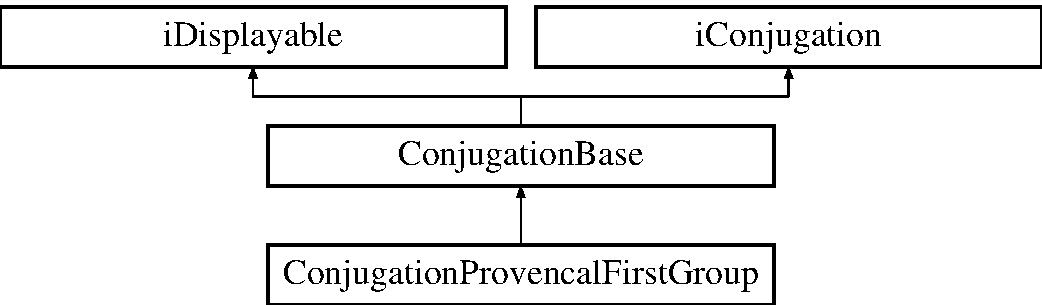
\includegraphics[height=3.000000cm]{classConjugationProvencalFirstGroup}
\end{center}
\end{figure}
\subsection*{Fonctions membres publiques}
\begin{DoxyCompactItemize}
\item 
\hypertarget{classConjugationProvencalFirstGroup_a6bd7d4bb8434586bf0ac5836a51d0022}{}\label{classConjugationProvencalFirstGroup_a6bd7d4bb8434586bf0ac5836a51d0022} 
{\bfseries display} ()
\end{DoxyCompactItemize}
\subsection*{Fonctions membres protégées}
\begin{DoxyCompactItemize}
\item 
\hypertarget{classConjugationProvencalFirstGroup_aedd116ac330b4c069c860612d624badc}{}\label{classConjugationProvencalFirstGroup_aedd116ac330b4c069c860612d624badc} 
{\bfseries get\+Standard\+Conjugation} ()
\item 
\hypertarget{classConjugationProvencalFirstGroup_a58519c759619a7566d20de71b6c93dc6}{}\label{classConjugationProvencalFirstGroup_a58519c759619a7566d20de71b6c93dc6} 
{\bfseries fix\+Radical} (\$radical, \$desinence)
\item 
\hypertarget{classConjugationProvencalFirstGroup_a65b702345db86895aecf34b88f0134a7}{}\label{classConjugationProvencalFirstGroup_a65b702345db86895aecf34b88f0134a7} 
{\bfseries fix\+Desinence} (\$desinence)
\item 
\hypertarget{classConjugationProvencalFirstGroup_a65f47dc174389bc9b680cef0a3e622a2}{}\label{classConjugationProvencalFirstGroup_a65f47dc174389bc9b680cef0a3e622a2} 
{\bfseries get\+Conjugation\+Array} ()
\item 
\hypertarget{classConjugationProvencalFirstGroup_a26ccc767ad4308637e382b4dd653f43a}{}\label{classConjugationProvencalFirstGroup_a26ccc767ad4308637e382b4dd653f43a} 
{\bfseries get\+Desinence\+Length\+Array} ()
\item 
\hypertarget{classConjugationProvencalFirstGroup_ad06866f3c378d109a3e56ff8a69d660a}{}\label{classConjugationProvencalFirstGroup_ad06866f3c378d109a3e56ff8a69d660a} 
{\bfseries conjugate} ()
\end{DoxyCompactItemize}
\subsection*{Membres hérités additionnels}


La documentation de cette classe a été générée à partir du fichier suivant \+:\begin{DoxyCompactItemize}
\item 
php/includes/Conjugation\+Provencal\+First\+Group.\+inc\end{DoxyCompactItemize}

\hypertarget{classConjugationProvencalManager}{}\section{Référence de la classe Conjugation\+Provencal\+Manager}
\label{classConjugationProvencalManager}\index{Conjugation\+Provencal\+Manager@{Conjugation\+Provencal\+Manager}}
Graphe d\textquotesingle{}héritage de Conjugation\+Provencal\+Manager\+:\begin{figure}[H]
\begin{center}
\leavevmode
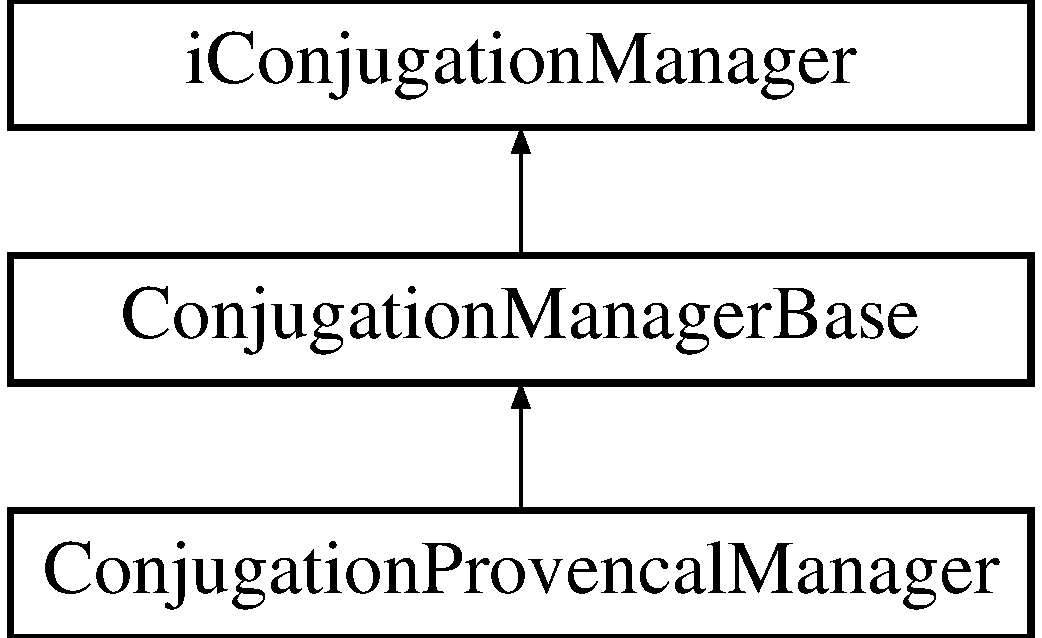
\includegraphics[height=3.000000cm]{classConjugationProvencalManager}
\end{center}
\end{figure}
\subsection*{Fonctions membres publiques}
\begin{DoxyCompactItemize}
\item 
\hypertarget{classConjugationProvencalManager_ab63e44b281c68e841becec69bf3abf5d}{}\label{classConjugationProvencalManager_ab63e44b281c68e841becec69bf3abf5d} 
{\bfseries generate\+Conjugation} ()
\item 
\hyperlink{classConjugationProvencalManager_ab54b1aaa7e39d3f31d416640322eae5a}{get\+Usual\+Verbs} ()
\item 
\hypertarget{classConjugationProvencalManager_acfdf3d08b4e9787cd9fac2e9eea042ba}{}\label{classConjugationProvencalManager_acfdf3d08b4e9787cd9fac2e9eea042ba} 
{\bfseries get\+Short\+Label} ()
\item 
\hypertarget{classConjugationProvencalManager_a9795549adf0ba2f9bded882cf85c792c}{}\label{classConjugationProvencalManager_a9795549adf0ba2f9bded882cf85c792c} 
{\bfseries get\+Long\+Label} ()
\end{DoxyCompactItemize}
\subsection*{Membres hérités additionnels}


\subsection{Documentation des fonctions membres}
\hypertarget{classConjugationProvencalManager_ab54b1aaa7e39d3f31d416640322eae5a}{}\label{classConjugationProvencalManager_ab54b1aaa7e39d3f31d416640322eae5a} 
\index{Conjugation\+Provencal\+Manager@{Conjugation\+Provencal\+Manager}!get\+Usual\+Verbs@{get\+Usual\+Verbs}}
\index{get\+Usual\+Verbs@{get\+Usual\+Verbs}!Conjugation\+Provencal\+Manager@{Conjugation\+Provencal\+Manager}}
\subsubsection{\texorpdfstring{get\+Usual\+Verbs()}{getUsualVerbs()}}
{\footnotesize\ttfamily Conjugation\+Provencal\+Manager\+::get\+Usual\+Verbs (\begin{DoxyParamCaption}{ }\end{DoxyParamCaption})}

\begin{DoxyReturn}{Renvoie}
an short array of verbs usually asked for. 
\end{DoxyReturn}


Implémente \hyperlink{interfaceiConjugationManager_a2a7ed39313c1c92ef5c01c88895de36e}{i\+Conjugation\+Manager}.



La documentation de cette classe a été générée à partir du fichier suivant \+:\begin{DoxyCompactItemize}
\item 
php/includes/Conjugation\+Provencal\+Manager.\+inc\end{DoxyCompactItemize}

\hypertarget{classConjugationProvencalSecondGroup}{}\section{Référence de la classe Conjugation\+Provencal\+Second\+Group}
\label{classConjugationProvencalSecondGroup}\index{Conjugation\+Provencal\+Second\+Group@{Conjugation\+Provencal\+Second\+Group}}
Graphe d\textquotesingle{}héritage de Conjugation\+Provencal\+Second\+Group\+:\begin{figure}[H]
\begin{center}
\leavevmode
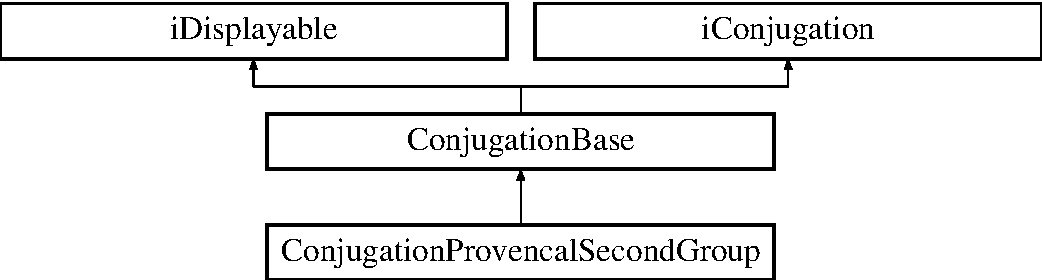
\includegraphics[height=3.000000cm]{classConjugationProvencalSecondGroup}
\end{center}
\end{figure}
\subsection*{Fonctions membres publiques}
\begin{DoxyCompactItemize}
\item 
\hypertarget{classConjugationProvencalSecondGroup_a99d29b0ed4e0e8129dfff0ed94746c4f}{}\label{classConjugationProvencalSecondGroup_a99d29b0ed4e0e8129dfff0ed94746c4f} 
{\bfseries display} ()
\end{DoxyCompactItemize}
\subsection*{Fonctions membres protégées}
\begin{DoxyCompactItemize}
\item 
\hypertarget{classConjugationProvencalSecondGroup_abe567700b32c8867ff9a5cd4d9777aec}{}\label{classConjugationProvencalSecondGroup_abe567700b32c8867ff9a5cd4d9777aec} 
{\bfseries get\+Standard\+Conjugation} ()
\item 
\hypertarget{classConjugationProvencalSecondGroup_a8e2552ef5ad24b15da6b0b294acf4ae1}{}\label{classConjugationProvencalSecondGroup_a8e2552ef5ad24b15da6b0b294acf4ae1} 
{\bfseries conjugate} ()
\end{DoxyCompactItemize}
\subsection*{Membres hérités additionnels}


La documentation de cette classe a été générée à partir du fichier suivant \+:\begin{DoxyCompactItemize}
\item 
php/includes/Conjugation\+Provencal\+Second\+Group.\+inc\end{DoxyCompactItemize}

\hypertarget{classConjugationProvencalThirdGroup}{}\section{Référence de la classe Conjugation\+Provencal\+Third\+Group}
\label{classConjugationProvencalThirdGroup}\index{Conjugation\+Provencal\+Third\+Group@{Conjugation\+Provencal\+Third\+Group}}
Graphe d\textquotesingle{}héritage de Conjugation\+Provencal\+Third\+Group\+:\begin{figure}[H]
\begin{center}
\leavevmode
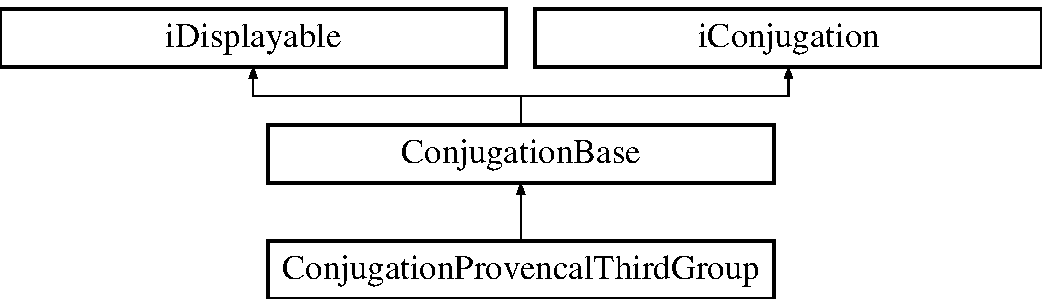
\includegraphics[height=3.000000cm]{classConjugationProvencalThirdGroup}
\end{center}
\end{figure}
\subsection*{Fonctions membres publiques}
\begin{DoxyCompactItemize}
\item 
\hypertarget{classConjugationProvencalThirdGroup_afed342691cc7dc2dd626040c8fa26774}{}\label{classConjugationProvencalThirdGroup_afed342691cc7dc2dd626040c8fa26774} 
{\bfseries \+\_\+\+\_\+construct} (Conjugation\+Manager \$manager, \$name, \$id, \$alias, \$model, \$comments, \$localization)
\item 
\hypertarget{classConjugationProvencalThirdGroup_a5be367146782812cba9ff8209cf79be2}{}\label{classConjugationProvencalThirdGroup_a5be367146782812cba9ff8209cf79be2} 
{\bfseries display} ()
\end{DoxyCompactItemize}
\subsection*{Fonctions membres protégées}
\begin{DoxyCompactItemize}
\item 
\hypertarget{classConjugationProvencalThirdGroup_ab4005ad44671e23386f8ef1f833b6959}{}\label{classConjugationProvencalThirdGroup_ab4005ad44671e23386f8ef1f833b6959} 
\hyperlink{classConjugationBase_a97684bf47a4b158a2d4f5716f9187730}{get\+Standard\+Conjugation}() {\bfseries conjugate} ()
\end{DoxyCompactItemize}
\subsection*{Membres hérités additionnels}


La documentation de cette classe a été générée à partir du fichier suivant \+:\begin{DoxyCompactItemize}
\item 
php/includes/Conjugation\+Provencal\+Third\+Group.\+inc\end{DoxyCompactItemize}

\hypertarget{classConverterCSV}{}\section{Référence de la classe Converter\+C\+SV}
\label{classConverterCSV}\index{Converter\+C\+SV@{Converter\+C\+SV}}
Graphe d\textquotesingle{}héritage de Converter\+C\+SV\+:\begin{figure}[H]
\begin{center}
\leavevmode
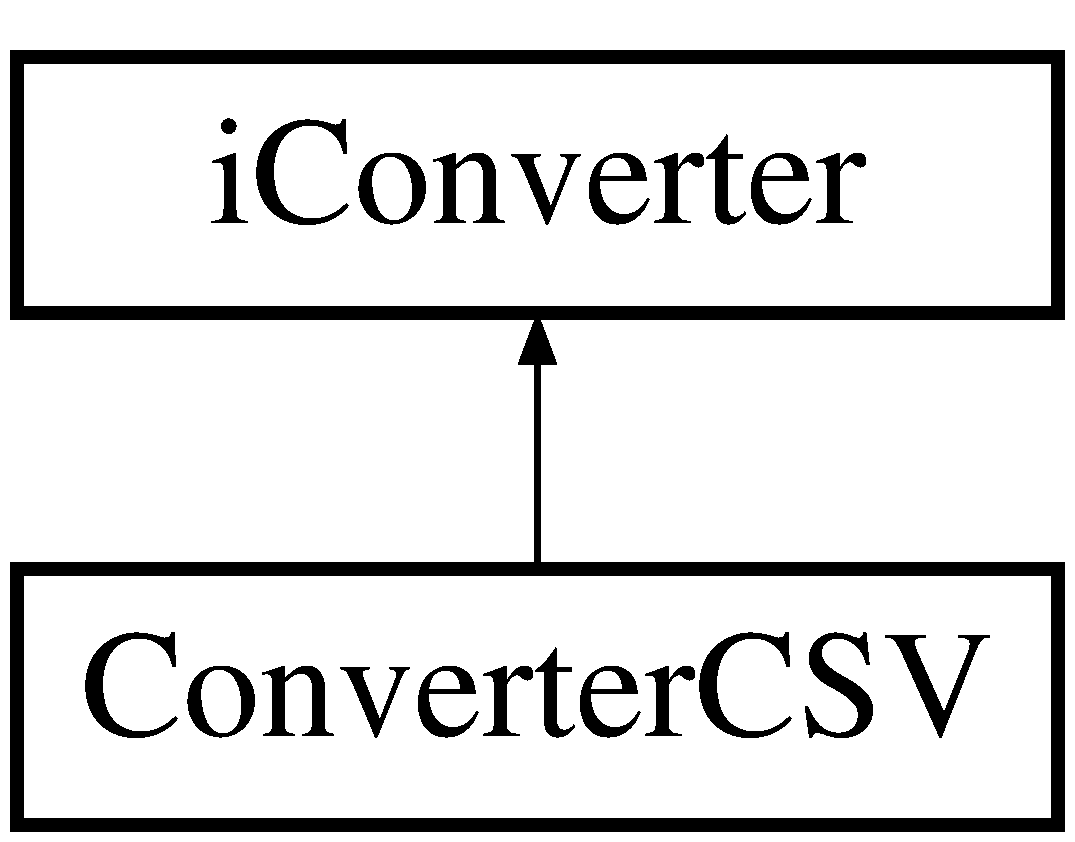
\includegraphics[height=2.000000cm]{classConverterCSV}
\end{center}
\end{figure}
\subsection*{Fonctions membres publiques}
\begin{DoxyCompactItemize}
\item 
\hyperlink{classConverterCSV_ad4fff7f9fd8e69926e394576558776f7}{\+\_\+\+\_\+construct} ()
\item 
\hyperlink{classConverterCSV_aff168b6953b8c9bdf43280c70e9c7170}{convert\+Conjugation} (array \$conjugated)
\item 
\hyperlink{classConverterCSV_a5bf7f48e54520210eeebdc2eb8f9e222}{convert\+Array} (array \$list)
\item 
\hypertarget{classConverterCSV_a36a4e52151f3326f7ed9f347dd30cdeb}{}\label{classConverterCSV_a36a4e52151f3326f7ed9f347dd30cdeb} 
{\bfseries convert\+Select} (array \$conjugation)
\item 
\hyperlink{classConverterCSV_a66253359624a5be3a4f5df9761b980a7}{convert\+Indexed\+Data} (\$data)
\end{DoxyCompactItemize}


\subsection{Documentation des constructeurs et destructeur}
\hypertarget{classConverterCSV_ad4fff7f9fd8e69926e394576558776f7}{}\label{classConverterCSV_ad4fff7f9fd8e69926e394576558776f7} 
\index{Converter\+C\+SV@{Converter\+C\+SV}!\+\_\+\+\_\+construct@{\+\_\+\+\_\+construct}}
\index{\+\_\+\+\_\+construct@{\+\_\+\+\_\+construct}!Converter\+C\+SV@{Converter\+C\+SV}}
\subsubsection{\texorpdfstring{\+\_\+\+\_\+construct()}{\_\_construct()}}
{\footnotesize\ttfamily Converter\+C\+S\+V\+::\+\_\+\+\_\+construct (\begin{DoxyParamCaption}{ }\end{DoxyParamCaption})}

does nothing 

\subsection{Documentation des fonctions membres}
\hypertarget{classConverterCSV_a5bf7f48e54520210eeebdc2eb8f9e222}{}\label{classConverterCSV_a5bf7f48e54520210eeebdc2eb8f9e222} 
\index{Converter\+C\+SV@{Converter\+C\+SV}!convert\+Array@{convert\+Array}}
\index{convert\+Array@{convert\+Array}!Converter\+C\+SV@{Converter\+C\+SV}}
\subsubsection{\texorpdfstring{convert\+Array()}{convertArray()}}
{\footnotesize\ttfamily Converter\+C\+S\+V\+::convert\+Array (\begin{DoxyParamCaption}\item[{array}]{\$list }\end{DoxyParamCaption})}

\begin{DoxyReturn}{Renvoie}
empty string 
\end{DoxyReturn}
\hypertarget{classConverterCSV_aff168b6953b8c9bdf43280c70e9c7170}{}\label{classConverterCSV_aff168b6953b8c9bdf43280c70e9c7170} 
\index{Converter\+C\+SV@{Converter\+C\+SV}!convert\+Conjugation@{convert\+Conjugation}}
\index{convert\+Conjugation@{convert\+Conjugation}!Converter\+C\+SV@{Converter\+C\+SV}}
\subsubsection{\texorpdfstring{convert\+Conjugation()}{convertConjugation()}}
{\footnotesize\ttfamily Converter\+C\+S\+V\+::convert\+Conjugation (\begin{DoxyParamCaption}\item[{array}]{\$conjugated }\end{DoxyParamCaption})}

\begin{DoxyReturn}{Renvoie}
empty string 
\end{DoxyReturn}
\hypertarget{classConverterCSV_a66253359624a5be3a4f5df9761b980a7}{}\label{classConverterCSV_a66253359624a5be3a4f5df9761b980a7} 
\index{Converter\+C\+SV@{Converter\+C\+SV}!convert\+Indexed\+Data@{convert\+Indexed\+Data}}
\index{convert\+Indexed\+Data@{convert\+Indexed\+Data}!Converter\+C\+SV@{Converter\+C\+SV}}
\subsubsection{\texorpdfstring{convert\+Indexed\+Data()}{convertIndexedData()}}
{\footnotesize\ttfamily Converter\+C\+S\+V\+::convert\+Indexed\+Data (\begin{DoxyParamCaption}\item[{}]{\$data }\end{DoxyParamCaption})}


\begin{DoxyParams}{Paramètres}
{\em \$data} & a Conjugation object \\
\hline
\end{DoxyParams}
\begin{DoxyReturn}{Renvoie}
a string in C\+SV format (data separated by semi-\/colon) 
\end{DoxyReturn}


La documentation de cette classe a été générée à partir du fichier suivant \+:\begin{DoxyCompactItemize}
\item 
php/includes/\hyperlink{ConverterCSV_8inc}{Converter\+C\+S\+V.\+inc}\end{DoxyCompactItemize}

\hypertarget{classConverterHTML}{}\section{Référence de la classe Converter\+H\+T\+ML}
\label{classConverterHTML}\index{Converter\+H\+T\+ML@{Converter\+H\+T\+ML}}
Graphe d\textquotesingle{}héritage de Converter\+H\+T\+ML\+:\begin{figure}[H]
\begin{center}
\leavevmode
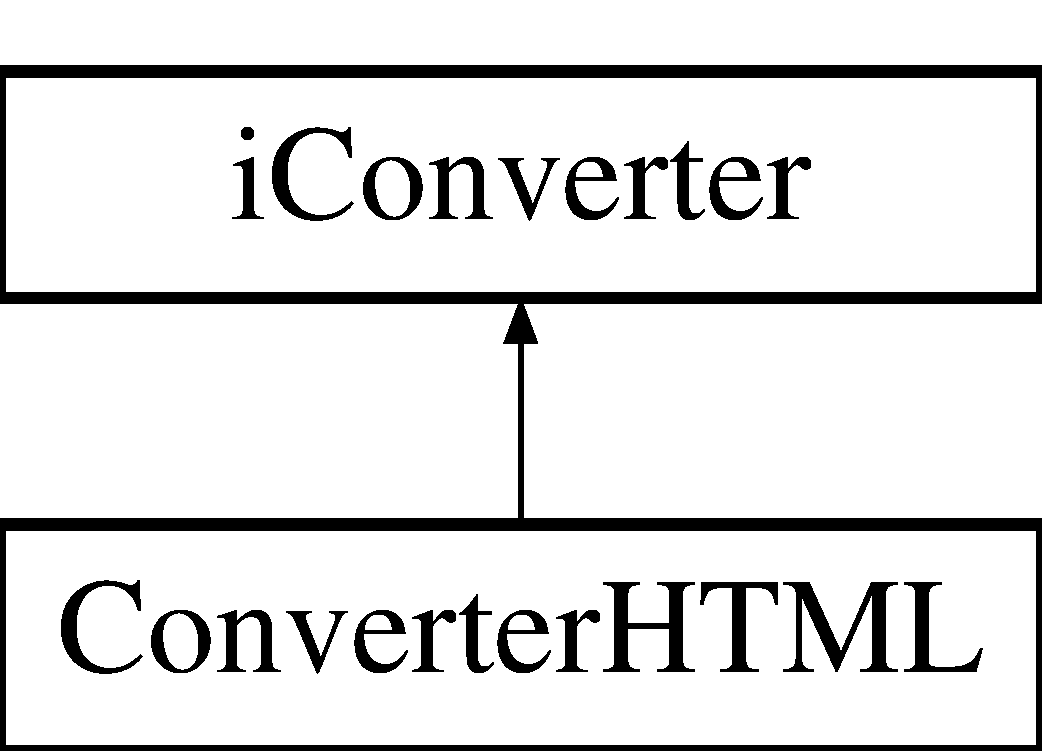
\includegraphics[height=2.000000cm]{classConverterHTML}
\end{center}
\end{figure}
\subsection*{Fonctions membres publiques}
\begin{DoxyCompactItemize}
\item 
\hypertarget{classConverterHTML_ad759ada61baaa9aa4f4c0f1d67182c05}{}\label{classConverterHTML_ad759ada61baaa9aa4f4c0f1d67182c05} 
{\bfseries convert\+Conjugation} (array \$conjugated)
\item 
\hypertarget{classConverterHTML_a62390602025ffe49e7b339a7782ddf72}{}\label{classConverterHTML_a62390602025ffe49e7b339a7782ddf72} 
{\bfseries convert\+Array} (array \$list)
\item 
\hypertarget{classConverterHTML_ae8152b5bc5d7a537c76e844df546dcbc}{}\label{classConverterHTML_ae8152b5bc5d7a537c76e844df546dcbc} 
{\bfseries convert\+Select} (array \$conjugation)
\item 
\hypertarget{classConverterHTML_a8cda80b6e1312b5f11e47fc719a511b3}{}\label{classConverterHTML_a8cda80b6e1312b5f11e47fc719a511b3} 
{\bfseries convert\+Indexed\+Data} (\$data)
\end{DoxyCompactItemize}
\subsection*{Fonctions membres protégées}
\begin{DoxyCompactItemize}
\item 
\hypertarget{classConverterHTML_a385bc4a802dc51c920ea5152df4adcb3}{}\label{classConverterHTML_a385bc4a802dc51c920ea5152df4adcb3} 
{\bfseries get\+Tempses} ()
\end{DoxyCompactItemize}


La documentation de cette classe a été générée à partir du fichier suivant \+:\begin{DoxyCompactItemize}
\item 
php/includes/Converter\+H\+T\+M\+L.\+inc\end{DoxyCompactItemize}

\hypertarget{classConverterIndexation}{}\section{Référence de la classe Converter\+Indexation}
\label{classConverterIndexation}\index{Converter\+Indexation@{Converter\+Indexation}}
Graphe d\textquotesingle{}héritage de Converter\+Indexation\+:\begin{figure}[H]
\begin{center}
\leavevmode
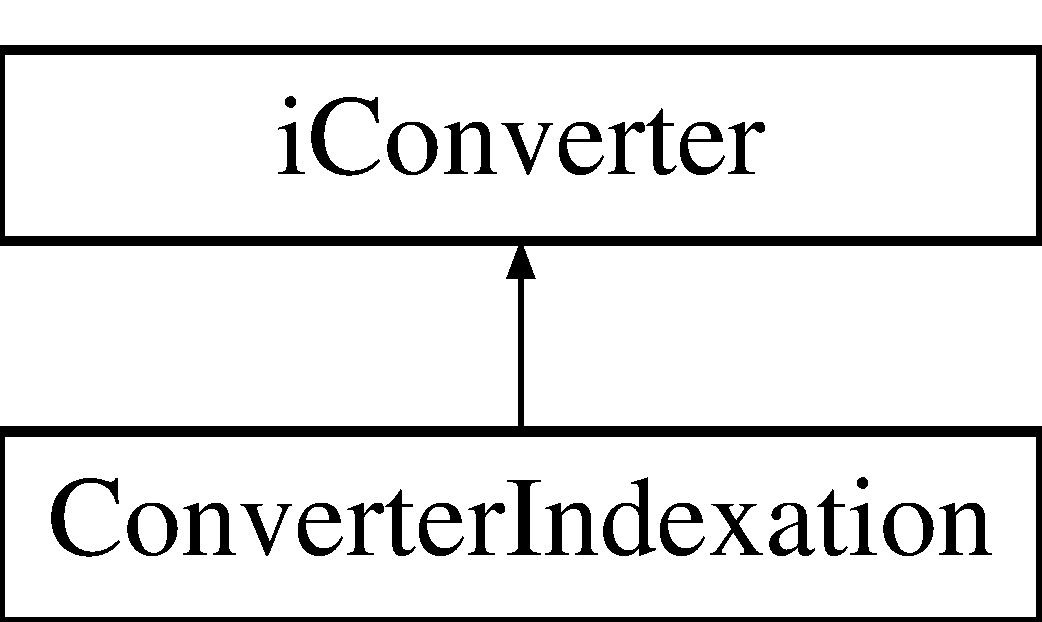
\includegraphics[height=2.000000cm]{classConverterIndexation}
\end{center}
\end{figure}
\subsection*{Fonctions membres publiques}
\begin{DoxyCompactItemize}
\item 
\hyperlink{classConverterIndexation_a8b52ecc585f7423456ae6aaf5df2436f}{encode\+P\+OS} (\$ary)
\begin{DoxyCompactList}\small\item\em takes an associative array and converts it to a P\+OS string in E\+A\+G\+L\+ES Morphosyntactic Annotation \end{DoxyCompactList}\item 
\hyperlink{classConverterIndexation_a6012e4df4619a7cc1c55c811fc50690d}{decode\+P\+OS} (\$pos)
\begin{DoxyCompactList}\small\item\em converts the P\+OS string into an human readable associative array \end{DoxyCompactList}\item 
\hyperlink{classConverterIndexation_ab9501f7ab3dad7daa338023522f03949}{encode\+Dialect} (\$str)
\begin{DoxyCompactList}\small\item\em converts the label of a dialect to its code \end{DoxyCompactList}\item 
\hyperlink{classConverterIndexation_a138e9e08f03d5a14fc53d367c9c739de}{decode\+Dialect} (\$str)
\begin{DoxyCompactList}\small\item\em converts the code of a dialect to its label \end{DoxyCompactList}\item 
\hyperlink{classConverterIndexation_aeabe347658ec9c09bf8ca65262ef6fa8}{encode\+Tense} (\$code)
\begin{DoxyCompactList}\small\item\em converts the code of a tense into its number/row \end{DoxyCompactList}\item 
\hyperlink{classConverterIndexation_a3d6b48ec5eaf46b9a2a8b3bdc200e063}{convert\+Conjugation} (array \$conjugated)
\item 
\hyperlink{classConverterIndexation_a171eb2b7d4d6452218212da881972dfd}{convert\+Array} (array \$ary)
\item 
\hyperlink{classConverterIndexation_a066755523513b6c4197765c631c7b248}{convert\+Select} (array \$conjugation)
\end{DoxyCompactItemize}


\subsection{Documentation des fonctions membres}
\hypertarget{classConverterIndexation_a171eb2b7d4d6452218212da881972dfd}{}\label{classConverterIndexation_a171eb2b7d4d6452218212da881972dfd} 
\index{Converter\+Indexation@{Converter\+Indexation}!convert\+Array@{convert\+Array}}
\index{convert\+Array@{convert\+Array}!Converter\+Indexation@{Converter\+Indexation}}
\subsubsection{\texorpdfstring{convert\+Array()}{convertArray()}}
{\footnotesize\ttfamily Converter\+Indexation\+::convert\+Array (\begin{DoxyParamCaption}\item[{array}]{\$ary }\end{DoxyParamCaption})}

\begin{DoxyReturn}{Renvoie}
an array converted 
\end{DoxyReturn}
\hypertarget{classConverterIndexation_a3d6b48ec5eaf46b9a2a8b3bdc200e063}{}\label{classConverterIndexation_a3d6b48ec5eaf46b9a2a8b3bdc200e063} 
\index{Converter\+Indexation@{Converter\+Indexation}!convert\+Conjugation@{convert\+Conjugation}}
\index{convert\+Conjugation@{convert\+Conjugation}!Converter\+Indexation@{Converter\+Indexation}}
\subsubsection{\texorpdfstring{convert\+Conjugation()}{convertConjugation()}}
{\footnotesize\ttfamily Converter\+Indexation\+::convert\+Conjugation (\begin{DoxyParamCaption}\item[{array}]{\$conjugated }\end{DoxyParamCaption})}


\begin{DoxyParams}{Paramètres}
{\em \$conjugated} & an array \\
\hline
\end{DoxyParams}
\begin{DoxyReturn}{Renvoie}
a array of a conjugated form from the indexation 
\end{DoxyReturn}
\hypertarget{classConverterIndexation_a066755523513b6c4197765c631c7b248}{}\label{classConverterIndexation_a066755523513b6c4197765c631c7b248} 
\index{Converter\+Indexation@{Converter\+Indexation}!convert\+Select@{convert\+Select}}
\index{convert\+Select@{convert\+Select}!Converter\+Indexation@{Converter\+Indexation}}
\subsubsection{\texorpdfstring{convert\+Select()}{convertSelect()}}
{\footnotesize\ttfamily Converter\+Indexation\+::convert\+Select (\begin{DoxyParamCaption}\item[{array}]{\$conjugation }\end{DoxyParamCaption})}

does nothing \hypertarget{classConverterIndexation_a138e9e08f03d5a14fc53d367c9c739de}{}\label{classConverterIndexation_a138e9e08f03d5a14fc53d367c9c739de} 
\index{Converter\+Indexation@{Converter\+Indexation}!decode\+Dialect@{decode\+Dialect}}
\index{decode\+Dialect@{decode\+Dialect}!Converter\+Indexation@{Converter\+Indexation}}
\subsubsection{\texorpdfstring{decode\+Dialect()}{decodeDialect()}}
{\footnotesize\ttfamily Converter\+Indexation\+::decode\+Dialect (\begin{DoxyParamCaption}\item[{}]{\$str }\end{DoxyParamCaption})}



converts the code of a dialect to its label 


\begin{DoxyParams}{Paramètres}
{\em \$str} & code for a dialect \\
\hline
\end{DoxyParams}
\begin{DoxySeeAlso}{Voir également}
\hyperlink{classConverterIndexation_ab9501f7ab3dad7daa338023522f03949}{encode\+Dialect()} 
\end{DoxySeeAlso}
\begin{DoxyReturn}{Renvoie}
the label of a dialect 
\end{DoxyReturn}
\hypertarget{classConverterIndexation_a6012e4df4619a7cc1c55c811fc50690d}{}\label{classConverterIndexation_a6012e4df4619a7cc1c55c811fc50690d} 
\index{Converter\+Indexation@{Converter\+Indexation}!decode\+P\+OS@{decode\+P\+OS}}
\index{decode\+P\+OS@{decode\+P\+OS}!Converter\+Indexation@{Converter\+Indexation}}
\subsubsection{\texorpdfstring{decode\+P\+O\+S()}{decodePOS()}}
{\footnotesize\ttfamily Converter\+Indexation\+::decode\+P\+OS (\begin{DoxyParamCaption}\item[{}]{\$pos }\end{DoxyParamCaption})}



converts the P\+OS string into an human readable associative array 


\begin{DoxyParams}{Paramètres}
{\em \$pos} & label for a dialect \\
\hline
\end{DoxyParams}
\begin{DoxySeeAlso}{Voir également}
\hyperlink{classConverterIndexation_a8b52ecc585f7423456ae6aaf5df2436f}{encode\+P\+O\+S()} 
\end{DoxySeeAlso}
\begin{DoxyReturn}{Renvoie}
an associative array of P\+OS human readable 
\end{DoxyReturn}
\hypertarget{classConverterIndexation_ab9501f7ab3dad7daa338023522f03949}{}\label{classConverterIndexation_ab9501f7ab3dad7daa338023522f03949} 
\index{Converter\+Indexation@{Converter\+Indexation}!encode\+Dialect@{encode\+Dialect}}
\index{encode\+Dialect@{encode\+Dialect}!Converter\+Indexation@{Converter\+Indexation}}
\subsubsection{\texorpdfstring{encode\+Dialect()}{encodeDialect()}}
{\footnotesize\ttfamily Converter\+Indexation\+::encode\+Dialect (\begin{DoxyParamCaption}\item[{}]{\$str }\end{DoxyParamCaption})}



converts the label of a dialect to its code 


\begin{DoxyParams}{Paramètres}
{\em \$str} & label for a dialect \\
\hline
\end{DoxyParams}
\begin{DoxySeeAlso}{Voir également}
\hyperlink{classConverterIndexation_a138e9e08f03d5a14fc53d367c9c739de}{decode\+Dialect()} 
\end{DoxySeeAlso}
\begin{DoxyReturn}{Renvoie}
the code of a dialect 
\end{DoxyReturn}
\hypertarget{classConverterIndexation_a8b52ecc585f7423456ae6aaf5df2436f}{}\label{classConverterIndexation_a8b52ecc585f7423456ae6aaf5df2436f} 
\index{Converter\+Indexation@{Converter\+Indexation}!encode\+P\+OS@{encode\+P\+OS}}
\index{encode\+P\+OS@{encode\+P\+OS}!Converter\+Indexation@{Converter\+Indexation}}
\subsubsection{\texorpdfstring{encode\+P\+O\+S()}{encodePOS()}}
{\footnotesize\ttfamily Converter\+Indexation\+::encode\+P\+OS (\begin{DoxyParamCaption}\item[{}]{\$ary }\end{DoxyParamCaption})}



takes an associative array and converts it to a P\+OS string in E\+A\+G\+L\+ES Morphosyntactic Annotation 


\begin{DoxyParams}{Paramètres}
{\em \$ary} & the associative array \\
\hline
\end{DoxyParams}
\begin{DoxySeeAlso}{Voir également}
\hyperlink{classConverterIndexation_a6012e4df4619a7cc1c55c811fc50690d}{decode\+P\+O\+S()} 
\end{DoxySeeAlso}
\begin{DoxyReturn}{Renvoie}
the P\+OS string 
\end{DoxyReturn}
\hypertarget{classConverterIndexation_aeabe347658ec9c09bf8ca65262ef6fa8}{}\label{classConverterIndexation_aeabe347658ec9c09bf8ca65262ef6fa8} 
\index{Converter\+Indexation@{Converter\+Indexation}!encode\+Tense@{encode\+Tense}}
\index{encode\+Tense@{encode\+Tense}!Converter\+Indexation@{Converter\+Indexation}}
\subsubsection{\texorpdfstring{encode\+Tense()}{encodeTense()}}
{\footnotesize\ttfamily Converter\+Indexation\+::encode\+Tense (\begin{DoxyParamCaption}\item[{}]{\$code }\end{DoxyParamCaption})}



converts the code of a tense into its number/row 


\begin{DoxyParams}{Paramètres}
{\em \$code} & for a tense \\
\hline
\end{DoxyParams}
\begin{DoxyReturn}{Renvoie}
the scalar of a tense 
\end{DoxyReturn}


La documentation de cette classe a été générée à partir du fichier suivant \+:\begin{DoxyCompactItemize}
\item 
php/includes/\hyperlink{ConverterIndexation_8inc}{Converter\+Indexation.\+inc}\end{DoxyCompactItemize}

\hypertarget{classConverterJSON}{}\section{Référence de la classe Converter\+J\+S\+ON}
\label{classConverterJSON}\index{Converter\+J\+S\+ON@{Converter\+J\+S\+ON}}
Graphe d\textquotesingle{}héritage de Converter\+J\+S\+ON\+:\begin{figure}[H]
\begin{center}
\leavevmode
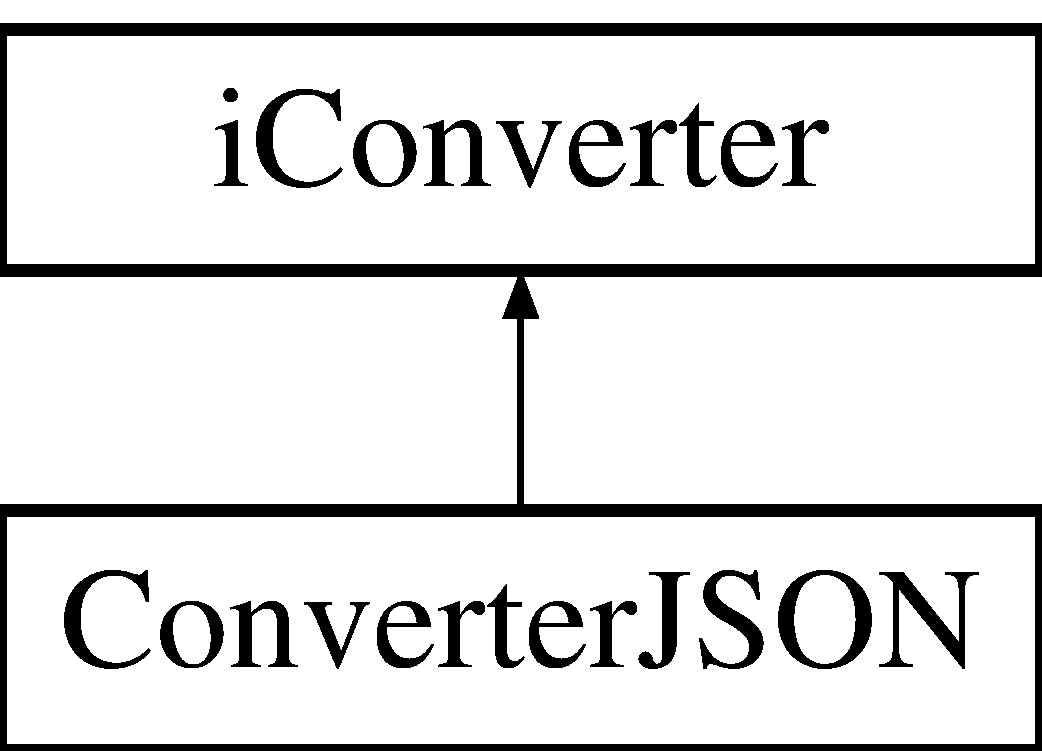
\includegraphics[height=2.000000cm]{classConverterJSON}
\end{center}
\end{figure}
\subsection*{Fonctions membres publiques}
\begin{DoxyCompactItemize}
\item 
\hypertarget{classConverterJSON_a245ad3051426af9af7cbc251642f0c90}{}\label{classConverterJSON_a245ad3051426af9af7cbc251642f0c90} 
{\bfseries convert\+Conjugation} (array \$conjugated)
\item 
\hypertarget{classConverterJSON_a3ed7ca94bfa42fdb952bcb360a7fd4ae}{}\label{classConverterJSON_a3ed7ca94bfa42fdb952bcb360a7fd4ae} 
{\bfseries convert\+Array} (array \$list)
\item 
\hypertarget{classConverterJSON_a62bbae5bb6a9aef4d648eddbe40fa16c}{}\label{classConverterJSON_a62bbae5bb6a9aef4d648eddbe40fa16c} 
{\bfseries convert\+Select} (array \$conjugation)
\item 
\hypertarget{classConverterJSON_a005d755a0798196fb1ec12e374b695c0}{}\label{classConverterJSON_a005d755a0798196fb1ec12e374b695c0} 
{\bfseries convert\+Indexed\+Data} (\$data)
\end{DoxyCompactItemize}


La documentation de cette classe a été générée à partir du fichier suivant \+:\begin{DoxyCompactItemize}
\item 
php/includes/Converter\+J\+S\+O\+N.\+inc\end{DoxyCompactItemize}

\hypertarget{classConverterLATEX}{}\section{Référence de la classe Converter\+L\+A\+T\+EX}
\label{classConverterLATEX}\index{Converter\+L\+A\+T\+EX@{Converter\+L\+A\+T\+EX}}
Graphe d\textquotesingle{}héritage de Converter\+L\+A\+T\+EX\+:\begin{figure}[H]
\begin{center}
\leavevmode
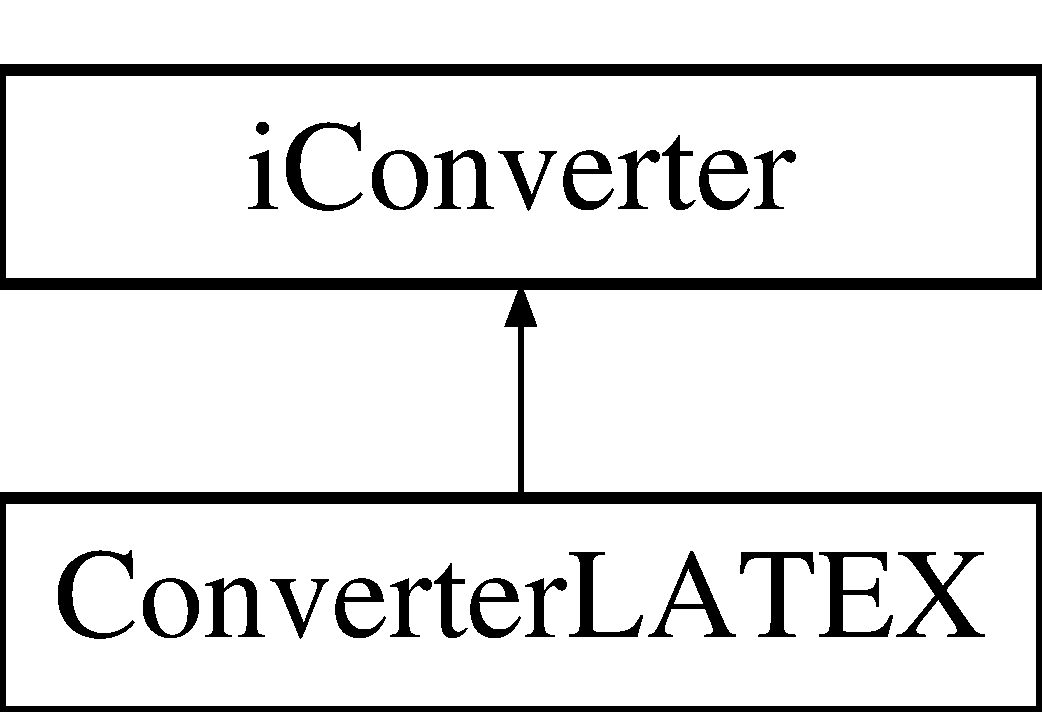
\includegraphics[height=2.000000cm]{classConverterLATEX}
\end{center}
\end{figure}
\subsection*{Fonctions membres publiques}
\begin{DoxyCompactItemize}
\item 
\hypertarget{classConverterLATEX_ada7781cb4daaf2f4a2f0c69e1d2f24e6}{}\label{classConverterLATEX_ada7781cb4daaf2f4a2f0c69e1d2f24e6} 
{\bfseries convert\+Conjugation} (array \$conjugated)
\item 
\hypertarget{classConverterLATEX_a1a30f6b145b4cb051d9dbbf8f9e8978f}{}\label{classConverterLATEX_a1a30f6b145b4cb051d9dbbf8f9e8978f} 
{\bfseries convert\+Array} (array \$list)
\item 
\hypertarget{classConverterLATEX_a21a5d5c23b40c7bb3b5cd7ebdbee3cae}{}\label{classConverterLATEX_a21a5d5c23b40c7bb3b5cd7ebdbee3cae} 
{\bfseries convert\+Select} (array \$conjugation)
\end{DoxyCompactItemize}
\subsection*{Attributs publics}
\begin{DoxyCompactItemize}
\item 
\hypertarget{classConverterLATEX_adaea9c0bff492f67f17ebe245ee889b1}{}\label{classConverterLATEX_adaea9c0bff492f67f17ebe245ee889b1} 
const {\bfseries F\+I\+L\+E\+C\+A\+C\+H\+I\+NG} = F\+A\+L\+SE
\end{DoxyCompactItemize}
\subsection*{Fonctions membres protégées}
\begin{DoxyCompactItemize}
\item 
\hypertarget{classConverterLATEX_a99d0b931aa33c2e4282c28f03b248e85}{}\label{classConverterLATEX_a99d0b931aa33c2e4282c28f03b248e85} 
{\bfseries get\+Tokens\+Array} ()
\item 
\hypertarget{classConverterLATEX_a5c2a6e5f6478af9a846f3b607c8d9105}{}\label{classConverterLATEX_a5c2a6e5f6478af9a846f3b607c8d9105} 
{\bfseries merge\+Tokens\+Array} (\&\$index, \&\$tokens, \$conjugation\+Arr)
\end{DoxyCompactItemize}


La documentation de cette classe a été générée à partir du fichier suivant \+:\begin{DoxyCompactItemize}
\item 
php/includes/\hyperlink{ConverterLATEX_8inc}{Converter\+L\+A\+T\+E\+X.\+inc}\end{DoxyCompactItemize}

\hypertarget{classConverterTEI}{}\section{Référence de la classe Converter\+T\+EI}
\label{classConverterTEI}\index{Converter\+T\+EI@{Converter\+T\+EI}}
Graphe d\textquotesingle{}héritage de Converter\+T\+EI\+:\begin{figure}[H]
\begin{center}
\leavevmode
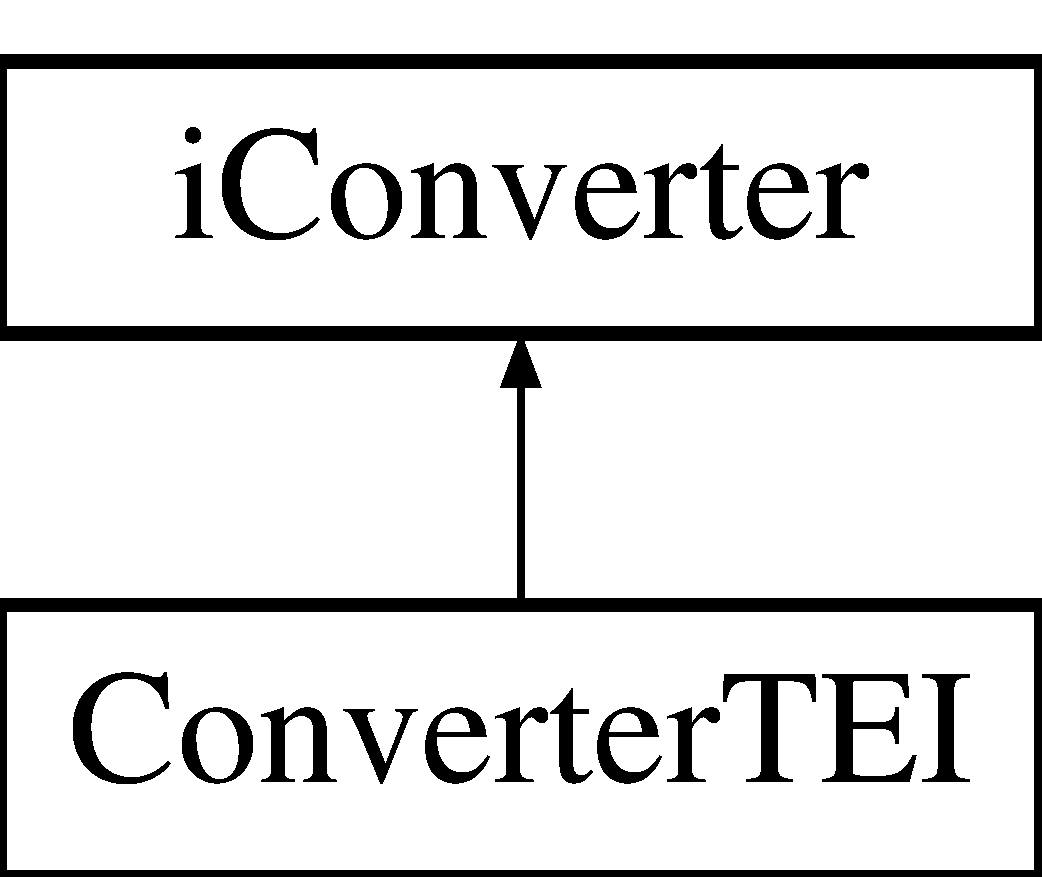
\includegraphics[height=2.000000cm]{classConverterTEI}
\end{center}
\end{figure}
\subsection*{Fonctions membres publiques}
\begin{DoxyCompactItemize}
\item 
\hypertarget{classConverterTEI_a13a33009d3a4829179627836450ea31a}{}\label{classConverterTEI_a13a33009d3a4829179627836450ea31a} 
\hyperlink{classConverterTEI_a13a33009d3a4829179627836450ea31a}{\+\_\+\+\_\+construct} ()
\begin{DoxyCompactList}\small\item\em Ctor. \end{DoxyCompactList}\item 
\hyperlink{classConverterTEI_a49fd33e0b0401c7bfaef1cca1bcee72c}{get\+Converter\+Indexation} ()
\item 
\hyperlink{classConverterTEI_a33798e9ea3e043efe980706e39e160d4}{convert\+Conjugation} (array \$conjugated)
\item 
\hypertarget{classConverterTEI_a3fcbf8ff1aa0399845dbec91faf17490}{}\label{classConverterTEI_a3fcbf8ff1aa0399845dbec91faf17490} 
{\bfseries convert\+Array} (array \$list)
\item 
\hypertarget{classConverterTEI_abb47b4d3c4c9d0787064f23a368ffa6d}{}\label{classConverterTEI_abb47b4d3c4c9d0787064f23a368ffa6d} 
{\bfseries convert\+Select} (array \$conjugation)
\end{DoxyCompactItemize}


\subsection{Documentation des fonctions membres}
\hypertarget{classConverterTEI_a33798e9ea3e043efe980706e39e160d4}{}\label{classConverterTEI_a33798e9ea3e043efe980706e39e160d4} 
\index{Converter\+T\+EI@{Converter\+T\+EI}!convert\+Conjugation@{convert\+Conjugation}}
\index{convert\+Conjugation@{convert\+Conjugation}!Converter\+T\+EI@{Converter\+T\+EI}}
\subsubsection{\texorpdfstring{convert\+Conjugation()}{convertConjugation()}}
{\footnotesize\ttfamily Converter\+T\+E\+I\+::convert\+Conjugation (\begin{DoxyParamCaption}\item[{array}]{\$conjugated }\end{DoxyParamCaption})}

returns a file to download w/ all the conjugation in T\+EI format 
\begin{DoxyParams}{Paramètres}
{\em \$conjugated} & a conjugation in array \\
\hline
\end{DoxyParams}
\hypertarget{classConverterTEI_a49fd33e0b0401c7bfaef1cca1bcee72c}{}\label{classConverterTEI_a49fd33e0b0401c7bfaef1cca1bcee72c} 
\index{Converter\+T\+EI@{Converter\+T\+EI}!get\+Converter\+Indexation@{get\+Converter\+Indexation}}
\index{get\+Converter\+Indexation@{get\+Converter\+Indexation}!Converter\+T\+EI@{Converter\+T\+EI}}
\subsubsection{\texorpdfstring{get\+Converter\+Indexation()}{getConverterIndexation()}}
{\footnotesize\ttfamily Converter\+T\+E\+I\+::get\+Converter\+Indexation (\begin{DoxyParamCaption}{ }\end{DoxyParamCaption})}

simple getter 

La documentation de cette classe a été générée à partir du fichier suivant \+:\begin{DoxyCompactItemize}
\item 
php/includes/\hyperlink{ConverterTEI_8inc}{Converter\+T\+E\+I.\+inc}\end{DoxyCompactItemize}

\hypertarget{classConverterXML}{}\section{Référence de la classe Converter\+X\+ML}
\label{classConverterXML}\index{Converter\+X\+ML@{Converter\+X\+ML}}
Graphe d\textquotesingle{}héritage de Converter\+X\+ML\+:\begin{figure}[H]
\begin{center}
\leavevmode
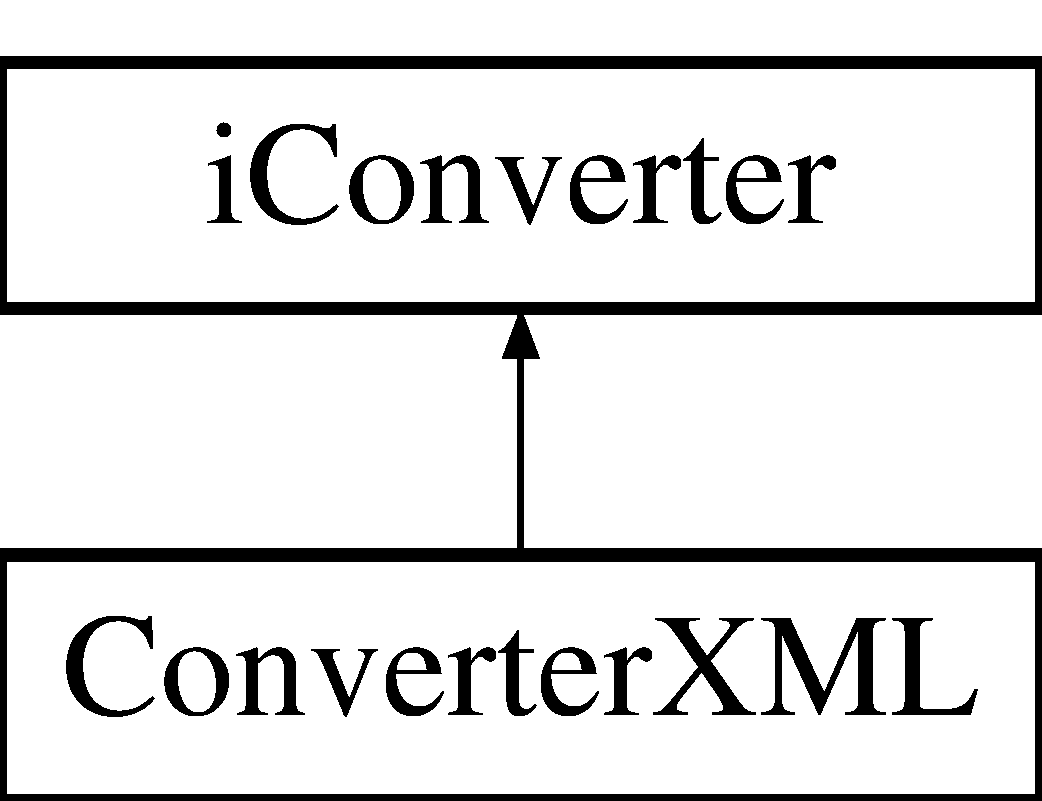
\includegraphics[height=2.000000cm]{classConverterXML}
\end{center}
\end{figure}
\subsection*{Fonctions membres publiques}
\begin{DoxyCompactItemize}
\item 
\hypertarget{classConverterXML_a17333b84c46af11e00e7bbd4e7001bf4}{}\label{classConverterXML_a17333b84c46af11e00e7bbd4e7001bf4} 
\hyperlink{classConverterXML_a17333b84c46af11e00e7bbd4e7001bf4}{\+\_\+\+\_\+construct} ()
\begin{DoxyCompactList}\small\item\em Ctor. \end{DoxyCompactList}\item 
\hyperlink{classConverterXML_a4c2d281657ce13ceb048b56824fec42a}{convert\+Conjugation} (array \$conjugated)
\item 
\hyperlink{classConverterXML_adfb936c9e38f4cee04c0c16db4aa1f34}{convert\+Array} (array \$list)
\item 
\hyperlink{classConverterXML_a68b03941080baea355f4d9c71743343e}{convert\+Select} (array \$conjugation)
\item 
\hyperlink{classConverterXML_ab7c370229f1693cea20750b07cc0d1e7}{convert\+Indexed\+Data} (\$data)
\end{DoxyCompactItemize}


\subsection{Documentation des fonctions membres}
\hypertarget{classConverterXML_adfb936c9e38f4cee04c0c16db4aa1f34}{}\label{classConverterXML_adfb936c9e38f4cee04c0c16db4aa1f34} 
\index{Converter\+X\+ML@{Converter\+X\+ML}!convert\+Array@{convert\+Array}}
\index{convert\+Array@{convert\+Array}!Converter\+X\+ML@{Converter\+X\+ML}}
\subsubsection{\texorpdfstring{convert\+Array()}{convertArray()}}
{\footnotesize\ttfamily Converter\+X\+M\+L\+::convert\+Array (\begin{DoxyParamCaption}\item[{array}]{\$list }\end{DoxyParamCaption})}


\begin{DoxyParams}{Paramètres}
{\em \$list} & a conjugation in array format \\
\hline
\end{DoxyParams}
\begin{DoxyReturn}{Renvoie}
an empty string 
\end{DoxyReturn}
\hypertarget{classConverterXML_a4c2d281657ce13ceb048b56824fec42a}{}\label{classConverterXML_a4c2d281657ce13ceb048b56824fec42a} 
\index{Converter\+X\+ML@{Converter\+X\+ML}!convert\+Conjugation@{convert\+Conjugation}}
\index{convert\+Conjugation@{convert\+Conjugation}!Converter\+X\+ML@{Converter\+X\+ML}}
\subsubsection{\texorpdfstring{convert\+Conjugation()}{convertConjugation()}}
{\footnotesize\ttfamily Converter\+X\+M\+L\+::convert\+Conjugation (\begin{DoxyParamCaption}\item[{array}]{\$conjugated }\end{DoxyParamCaption})}


\begin{DoxyParams}{Paramètres}
{\em \$conjugated} & \\
\hline
\end{DoxyParams}
\begin{DoxyReturn}{Renvoie}
a string empty 
\end{DoxyReturn}
\hypertarget{classConverterXML_ab7c370229f1693cea20750b07cc0d1e7}{}\label{classConverterXML_ab7c370229f1693cea20750b07cc0d1e7} 
\index{Converter\+X\+ML@{Converter\+X\+ML}!convert\+Indexed\+Data@{convert\+Indexed\+Data}}
\index{convert\+Indexed\+Data@{convert\+Indexed\+Data}!Converter\+X\+ML@{Converter\+X\+ML}}
\subsubsection{\texorpdfstring{convert\+Indexed\+Data()}{convertIndexedData()}}
{\footnotesize\ttfamily Converter\+X\+M\+L\+::convert\+Indexed\+Data (\begin{DoxyParamCaption}\item[{}]{\$data }\end{DoxyParamCaption})}


\begin{DoxyParams}{Paramètres}
{\em \$data} & an conjugation object \\
\hline
\end{DoxyParams}
\begin{DoxyReturn}{Renvoie}
an X\+ML string fully formatted 
\end{DoxyReturn}
$<$ this function call exits to let the navigator download the newly created file \hypertarget{classConverterXML_a68b03941080baea355f4d9c71743343e}{}\label{classConverterXML_a68b03941080baea355f4d9c71743343e} 
\index{Converter\+X\+ML@{Converter\+X\+ML}!convert\+Select@{convert\+Select}}
\index{convert\+Select@{convert\+Select}!Converter\+X\+ML@{Converter\+X\+ML}}
\subsubsection{\texorpdfstring{convert\+Select()}{convertSelect()}}
{\footnotesize\ttfamily Converter\+X\+M\+L\+::convert\+Select (\begin{DoxyParamCaption}\item[{array}]{\$conjugation }\end{DoxyParamCaption})}

\begin{DoxyReturn}{Renvoie}
an empty string 
\end{DoxyReturn}


La documentation de cette classe a été générée à partir du fichier suivant \+:\begin{DoxyCompactItemize}
\item 
php/includes/Converter\+X\+M\+L.\+inc\end{DoxyCompactItemize}

\hypertarget{interfaceiConjugation}{}\section{Référence de l\textquotesingle{}interface i\+Conjugation}
\label{interfaceiConjugation}\index{i\+Conjugation@{i\+Conjugation}}
Graphe d\textquotesingle{}héritage de i\+Conjugation\+:\begin{figure}[H]
\begin{center}
\leavevmode
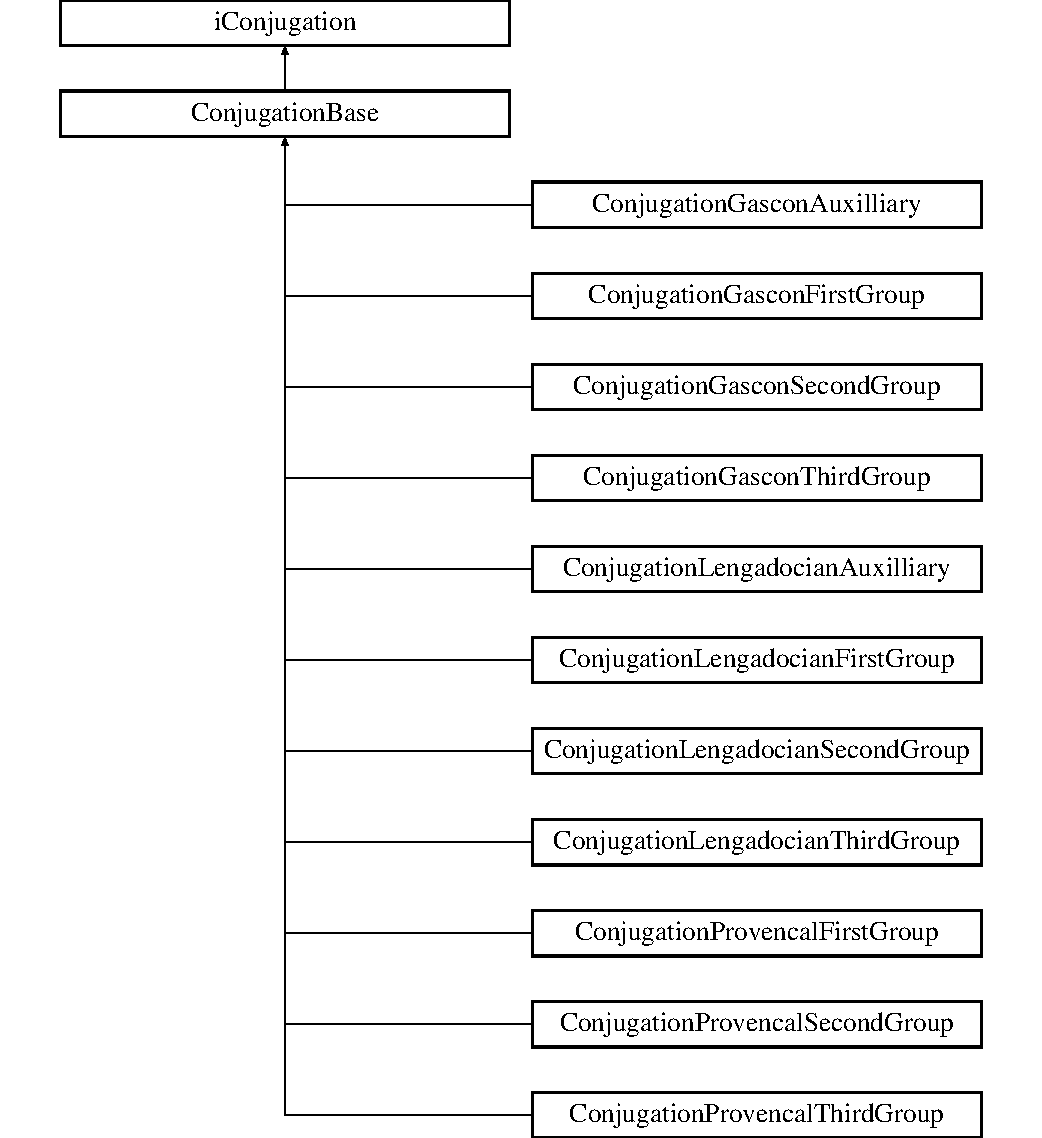
\includegraphics[height=12.000000cm]{interfaceiConjugation}
\end{center}
\end{figure}
\subsection*{Fonctions membres publiques}
\begin{DoxyCompactItemize}
\item 
\hyperlink{interfaceiConjugation_ab13cedc1b4f0d064a9bfff3cbfb63de6}{get\+Dictionary\+Definition} ()
\item 
\hyperlink{interfaceiConjugation_a21390064de33a77b99b26ec5a2e55351}{get\+Group} ()
\item 
\hypertarget{interfaceiConjugation_a5742a474f6114e172337a38ca2c8bae8}{}\label{interfaceiConjugation_a5742a474f6114e172337a38ca2c8bae8} 
{\bfseries get\+Verb} ()
\item 
\hyperlink{interfaceiConjugation_ab5482cc8f8e9f58dc852aff604813b6e}{get\+Verb\+Model} ()
\item 
\hypertarget{interfaceiConjugation_ab076acd6674f8effbf5306d6b92f3ad3}{}\label{interfaceiConjugation_ab076acd6674f8effbf5306d6b92f3ad3} 
{\bfseries get\+Verb\+Model\+Object} (\$nummodel)
\item 
\hyperlink{interfaceiConjugation_a2b6dd0a979a98bc50f6f9f7ec9b69e63}{getlib\+Model} ()
\item 
\hypertarget{interfaceiConjugation_ad887ef20e584040fe72f6e5a6212247e}{}\label{interfaceiConjugation_ad887ef20e584040fe72f6e5a6212247e} 
{\bfseries get\+Comments} ()
\item 
\hyperlink{interfaceiConjugation_a448829b47813a79d1f8ec65de91e8696}{get\+Manager} ()
\item 
\hyperlink{interfaceiConjugation_aa34e7af66125d28af4f485529d456a74}{get\+Verb\+Id} ()
\item 
\hyperlink{interfaceiConjugation_ab19ceb5ab295fd3d0f862d963379a7e2}{get\+Localization} ()
\item 
\hyperlink{interfaceiConjugation_a30a8959865d6b8d3f4ae69c31792f32a}{get\+Alias} ()
\item 
\hyperlink{interfaceiConjugation_a58e61c703ad1f0d76db1535235e530a0}{get\+See\+Also} ()
\item 
\hyperlink{interfaceiConjugation_a4e0b6c0923ecd596b6acff6c7b776f5f}{get\+Dialect} ()
\item 
\hyperlink{interfaceiConjugation_a6c0072d898eb8b2f3756c87dfed4af33}{get\+Conjugations} ()
\end{DoxyCompactItemize}


\subsection{Documentation des fonctions membres}
\hypertarget{interfaceiConjugation_a30a8959865d6b8d3f4ae69c31792f32a}{}\label{interfaceiConjugation_a30a8959865d6b8d3f4ae69c31792f32a} 
\index{i\+Conjugation@{i\+Conjugation}!get\+Alias@{get\+Alias}}
\index{get\+Alias@{get\+Alias}!i\+Conjugation@{i\+Conjugation}}
\subsubsection{\texorpdfstring{get\+Alias()}{getAlias()}}
{\footnotesize\ttfamily i\+Conjugation\+::get\+Alias (\begin{DoxyParamCaption}{ }\end{DoxyParamCaption})}

\begin{DoxyReturn}{Renvoie}
an id of the verb to be conjugated instead of this infinitive, in this case the infinitive is only a placeholder 
\end{DoxyReturn}


Implémenté dans \hyperlink{classConjugationBase_ac8266b933fde0f494a7933c4d2fe0590}{Conjugation\+Base}.

\hypertarget{interfaceiConjugation_a6c0072d898eb8b2f3756c87dfed4af33}{}\label{interfaceiConjugation_a6c0072d898eb8b2f3756c87dfed4af33} 
\index{i\+Conjugation@{i\+Conjugation}!get\+Conjugations@{get\+Conjugations}}
\index{get\+Conjugations@{get\+Conjugations}!i\+Conjugation@{i\+Conjugation}}
\subsubsection{\texorpdfstring{get\+Conjugations()}{getConjugations()}}
{\footnotesize\ttfamily i\+Conjugation\+::get\+Conjugations (\begin{DoxyParamCaption}{ }\end{DoxyParamCaption})}

\begin{DoxyReturn}{Renvoie}
an associative array of the object content 
\end{DoxyReturn}


Implémenté dans \hyperlink{classConjugationBase_ae5b10d1201dfc7ed1c56b1f5a073bbdb}{Conjugation\+Base}.

\hypertarget{interfaceiConjugation_a4e0b6c0923ecd596b6acff6c7b776f5f}{}\label{interfaceiConjugation_a4e0b6c0923ecd596b6acff6c7b776f5f} 
\index{i\+Conjugation@{i\+Conjugation}!get\+Dialect@{get\+Dialect}}
\index{get\+Dialect@{get\+Dialect}!i\+Conjugation@{i\+Conjugation}}
\subsubsection{\texorpdfstring{get\+Dialect()}{getDialect()}}
{\footnotesize\ttfamily i\+Conjugation\+::get\+Dialect (\begin{DoxyParamCaption}{ }\end{DoxyParamCaption})}

\begin{DoxyReturn}{Renvoie}
a string of the dialect in its short form 
\end{DoxyReturn}


Implémenté dans \hyperlink{classConjugationBase_a5010621a363fcfe26e5d23ade06d2c41}{Conjugation\+Base}.

\hypertarget{interfaceiConjugation_ab13cedc1b4f0d064a9bfff3cbfb63de6}{}\label{interfaceiConjugation_ab13cedc1b4f0d064a9bfff3cbfb63de6} 
\index{i\+Conjugation@{i\+Conjugation}!get\+Dictionary\+Definition@{get\+Dictionary\+Definition}}
\index{get\+Dictionary\+Definition@{get\+Dictionary\+Definition}!i\+Conjugation@{i\+Conjugation}}
\subsubsection{\texorpdfstring{get\+Dictionary\+Definition()}{getDictionaryDefinition()}}
{\footnotesize\ttfamily i\+Conjugation\+::get\+Dictionary\+Definition (\begin{DoxyParamCaption}{ }\end{DoxyParamCaption})}

\begin{DoxyReturn}{Renvoie}
a string, the definition of the verb infinitive 
\end{DoxyReturn}


Implémenté dans \hyperlink{classConjugationBase_aae493e154b07045a3ea072760ac44ef4}{Conjugation\+Base}.

\hypertarget{interfaceiConjugation_a21390064de33a77b99b26ec5a2e55351}{}\label{interfaceiConjugation_a21390064de33a77b99b26ec5a2e55351} 
\index{i\+Conjugation@{i\+Conjugation}!get\+Group@{get\+Group}}
\index{get\+Group@{get\+Group}!i\+Conjugation@{i\+Conjugation}}
\subsubsection{\texorpdfstring{get\+Group()}{getGroup()}}
{\footnotesize\ttfamily i\+Conjugation\+::get\+Group (\begin{DoxyParamCaption}{ }\end{DoxyParamCaption})}

\begin{DoxyReturn}{Renvoie}
a string, the verbal group 
\end{DoxyReturn}


Implémenté dans \hyperlink{classConjugationBase_aa88c93007f333b916a6a51819e50e8ae}{Conjugation\+Base}.

\hypertarget{interfaceiConjugation_a2b6dd0a979a98bc50f6f9f7ec9b69e63}{}\label{interfaceiConjugation_a2b6dd0a979a98bc50f6f9f7ec9b69e63} 
\index{i\+Conjugation@{i\+Conjugation}!getlib\+Model@{getlib\+Model}}
\index{getlib\+Model@{getlib\+Model}!i\+Conjugation@{i\+Conjugation}}
\subsubsection{\texorpdfstring{getlib\+Model()}{getlibModel()}}
{\footnotesize\ttfamily i\+Conjugation\+::getlib\+Model (\begin{DoxyParamCaption}{ }\end{DoxyParamCaption})}

\begin{DoxyReturn}{Renvoie}
a string, the label of the model (i.\+e \char`\"{}conjugason 1 non alternanta, iat Espii, espia, espiam, espièi, espiat\char`\"{}) 
\end{DoxyReturn}


Implémenté dans \hyperlink{classConjugationBase_a52db22137154c2fd7a8487406b959652}{Conjugation\+Base}.

\hypertarget{interfaceiConjugation_ab19ceb5ab295fd3d0f862d963379a7e2}{}\label{interfaceiConjugation_ab19ceb5ab295fd3d0f862d963379a7e2} 
\index{i\+Conjugation@{i\+Conjugation}!get\+Localization@{get\+Localization}}
\index{get\+Localization@{get\+Localization}!i\+Conjugation@{i\+Conjugation}}
\subsubsection{\texorpdfstring{get\+Localization()}{getLocalization()}}
{\footnotesize\ttfamily i\+Conjugation\+::get\+Localization (\begin{DoxyParamCaption}{ }\end{DoxyParamCaption})}

\begin{DoxyReturn}{Renvoie}
a string the localization of this conjugation (to be developped) 
\end{DoxyReturn}


Implémenté dans \hyperlink{classConjugationBase_a27cc8f5f2a3b502e48c22a5b547181ac}{Conjugation\+Base}.

\hypertarget{interfaceiConjugation_a448829b47813a79d1f8ec65de91e8696}{}\label{interfaceiConjugation_a448829b47813a79d1f8ec65de91e8696} 
\index{i\+Conjugation@{i\+Conjugation}!get\+Manager@{get\+Manager}}
\index{get\+Manager@{get\+Manager}!i\+Conjugation@{i\+Conjugation}}
\subsubsection{\texorpdfstring{get\+Manager()}{getManager()}}
{\footnotesize\ttfamily i\+Conjugation\+::get\+Manager (\begin{DoxyParamCaption}{ }\end{DoxyParamCaption})}

\begin{DoxyReturn}{Renvoie}
the manager
\end{DoxyReturn}
\begin{DoxyRefDesc}{A faire}
\item[\hyperlink{todo__todo000001}{A faire}](not supposed to be public) \end{DoxyRefDesc}


Implémenté dans \hyperlink{classConjugationBase_aab285eff4995c059a3aa0abec778a390}{Conjugation\+Base}.

\hypertarget{interfaceiConjugation_a58e61c703ad1f0d76db1535235e530a0}{}\label{interfaceiConjugation_a58e61c703ad1f0d76db1535235e530a0} 
\index{i\+Conjugation@{i\+Conjugation}!get\+See\+Also@{get\+See\+Also}}
\index{get\+See\+Also@{get\+See\+Also}!i\+Conjugation@{i\+Conjugation}}
\subsubsection{\texorpdfstring{get\+See\+Also()}{getSeeAlso()}}
{\footnotesize\ttfamily i\+Conjugation\+::get\+See\+Also (\begin{DoxyParamCaption}{ }\end{DoxyParamCaption})}

\begin{DoxyReturn}{Renvoie}
a string, an infinitive of the verb recommended instead of this one 
\end{DoxyReturn}


Implémenté dans \hyperlink{classConjugationBase_a76d7179c150a4e32fb410d5af9bc388c}{Conjugation\+Base}.

\hypertarget{interfaceiConjugation_aa34e7af66125d28af4f485529d456a74}{}\label{interfaceiConjugation_aa34e7af66125d28af4f485529d456a74} 
\index{i\+Conjugation@{i\+Conjugation}!get\+Verb\+Id@{get\+Verb\+Id}}
\index{get\+Verb\+Id@{get\+Verb\+Id}!i\+Conjugation@{i\+Conjugation}}
\subsubsection{\texorpdfstring{get\+Verb\+Id()}{getVerbId()}}
{\footnotesize\ttfamily i\+Conjugation\+::get\+Verb\+Id (\begin{DoxyParamCaption}{ }\end{DoxyParamCaption})}

\begin{DoxyReturn}{Renvoie}
a string the id of the verb 
\end{DoxyReturn}


Implémenté dans \hyperlink{classConjugationBase_a918aff5acf4210cf363a13cf39e2430d}{Conjugation\+Base}.

\hypertarget{interfaceiConjugation_ab5482cc8f8e9f58dc852aff604813b6e}{}\label{interfaceiConjugation_ab5482cc8f8e9f58dc852aff604813b6e} 
\index{i\+Conjugation@{i\+Conjugation}!get\+Verb\+Model@{get\+Verb\+Model}}
\index{get\+Verb\+Model@{get\+Verb\+Model}!i\+Conjugation@{i\+Conjugation}}
\subsubsection{\texorpdfstring{get\+Verb\+Model()}{getVerbModel()}}
{\footnotesize\ttfamily i\+Conjugation\+::get\+Verb\+Model (\begin{DoxyParamCaption}{ }\end{DoxyParamCaption})}

\begin{DoxyReturn}{Renvoie}
a string, the verb model (a standardized form i.\+e \char`\"{}105 d\char`\"{}) 
\end{DoxyReturn}


Implémenté dans \hyperlink{classConjugationBase_aaa7ecb3341682d48f2d2b42810de2ac2}{Conjugation\+Base}.



La documentation de cette interface a été générée à partir du fichier suivant \+:\begin{DoxyCompactItemize}
\item 
php/includes/i\+Conjugation.\+inc\end{DoxyCompactItemize}

\hypertarget{interfaceIConjugationDataProvider}{}\section{Référence de l\textquotesingle{}interface I\+Conjugation\+Data\+Provider}
\label{interfaceIConjugationDataProvider}\index{I\+Conjugation\+Data\+Provider@{I\+Conjugation\+Data\+Provider}}
\subsection*{Fonctions membres publiques}
\begin{DoxyCompactItemize}
\item 
\hypertarget{interfaceIConjugationDataProvider_a528f3344f0463077e305886ebcc031a6}{}\label{interfaceIConjugationDataProvider_a528f3344f0463077e305886ebcc031a6} 
{\bfseries get\+Verb} (\$verb)
\item 
\hypertarget{interfaceIConjugationDataProvider_a60a3d72a92a67f89a93b8396ea5edd0d}{}\label{interfaceIConjugationDataProvider_a60a3d72a92a67f89a93b8396ea5edd0d} 
{\bfseries get\+Verb\+By\+Id} (\$id)
\item 
\hypertarget{interfaceIConjugationDataProvider_abdf3d3ed8eb4045b80461a880c0a3e24}{}\label{interfaceIConjugationDataProvider_abdf3d3ed8eb4045b80461a880c0a3e24} 
{\bfseries get\+Verb\+Model\+Object} (\$num\+Model)
\item 
\hypertarget{interfaceIConjugationDataProvider_a96c98a3a99a79c0a4228a585c5294576}{}\label{interfaceIConjugationDataProvider_a96c98a3a99a79c0a4228a585c5294576} 
{\bfseries get\+Top20} ()
\item 
\hypertarget{interfaceIConjugationDataProvider_a5c7f6041f670ef5560f72577f5f25867}{}\label{interfaceIConjugationDataProvider_a5c7f6041f670ef5560f72577f5f25867} 
{\bfseries get\+Others\+In\+Model} (\$verb)
\item 
\hypertarget{interfaceIConjugationDataProvider_a62018b8fae6510989ebcb9c974958586}{}\label{interfaceIConjugationDataProvider_a62018b8fae6510989ebcb9c974958586} 
{\bfseries get\+Count\+Others\+In\+Model} (\$verb)
\item 
\hypertarget{interfaceIConjugationDataProvider_abc704f44a3eaec66a9d2461c9be1240b}{}\label{interfaceIConjugationDataProvider_abc704f44a3eaec66a9d2461c9be1240b} 
{\bfseries get\+Verb\+Auto\+Complete} (\$string)
\item 
\hypertarget{interfaceIConjugationDataProvider_a254299b72e84b00aec82d4037d484666}{}\label{interfaceIConjugationDataProvider_a254299b72e84b00aec82d4037d484666} 
{\bfseries get\+Random\+Verb} ()
\item 
\hypertarget{interfaceIConjugationDataProvider_ac409d7c67841ef17b3aecaf330b9e675}{}\label{interfaceIConjugationDataProvider_ac409d7c67841ef17b3aecaf330b9e675} 
{\bfseries get\+Single\+Verbs} ()
\item 
\hypertarget{interfaceIConjugationDataProvider_acd3b7b4f960ad952b0c4e929d02c8923}{}\label{interfaceIConjugationDataProvider_acd3b7b4f960ad952b0c4e929d02c8923} 
{\bfseries get\+All\+Verbs} ()
\item 
\hypertarget{interfaceIConjugationDataProvider_a4526378019b6276cb91e64bddd3b1d77}{}\label{interfaceIConjugationDataProvider_a4526378019b6276cb91e64bddd3b1d77} 
{\bfseries get\+All\+Duplicated\+Verbs} ()
\item 
\hypertarget{interfaceIConjugationDataProvider_ac37a4f6f2def34dea3f008dce50bf41d}{}\label{interfaceIConjugationDataProvider_ac37a4f6f2def34dea3f008dce50bf41d} 
{\bfseries insert\+Indexed\+Verb} (array \$arr)
\item 
\hypertarget{interfaceIConjugationDataProvider_a1de2fd05896540e0e4e1f50631a2e86b}{}\label{interfaceIConjugationDataProvider_a1de2fd05896540e0e4e1f50631a2e86b} 
{\bfseries get\+Verbs\+Models} ()
\item 
\hypertarget{interfaceIConjugationDataProvider_aa30e7166c6d8e812482d6e420e05cc6c}{}\label{interfaceIConjugationDataProvider_aa30e7166c6d8e812482d6e420e05cc6c} 
{\bfseries get\+Verbs\+Models\+Mixed} ()
\end{DoxyCompactItemize}


La documentation de cette interface a été générée à partir du fichier suivant \+:\begin{DoxyCompactItemize}
\item 
php/includes/i\+Conjugation\+Data\+Provider.\+inc\end{DoxyCompactItemize}

\hypertarget{interfaceiConjugationManager}{}\section{Référence de l\textquotesingle{}interface i\+Conjugation\+Manager}
\label{interfaceiConjugationManager}\index{i\+Conjugation\+Manager@{i\+Conjugation\+Manager}}
Graphe d\textquotesingle{}héritage de i\+Conjugation\+Manager\+:\begin{figure}[H]
\begin{center}
\leavevmode
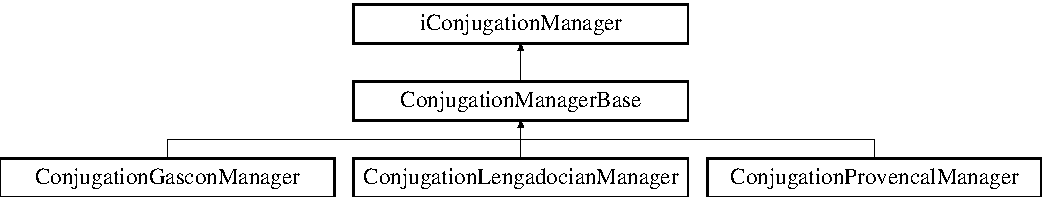
\includegraphics[height=2.654028cm]{interfaceiConjugationManager}
\end{center}
\end{figure}
\subsection*{Fonctions membres publiques}
\begin{DoxyCompactItemize}
\item 
\hyperlink{interfaceiConjugationManager_a2e955e8c88d45869683005343cbfac60}{get\+Random\+Verb} ()
\item 
\hyperlink{interfaceiConjugationManager_a2a7ed39313c1c92ef5c01c88895de36e}{get\+Usual\+Verbs} ()
\item 
\hyperlink{interfaceiConjugationManager_afba24324d7c48d3ab00ffba63cbc1b9e}{conjugate} ()
\begin{DoxyCompactList}\small\item\em immediatly called after setting a verb. \end{DoxyCompactList}\item 
\hyperlink{interfaceiConjugationManager_a1b56822fc7f5f7b7b9c0b0c406993b3c}{set\+Verb} (\$verb)
\item 
\hyperlink{interfaceiConjugationManager_a0273fc00cbbf9e83823d571e3e2c8945}{get\+Top20} ()
\end{DoxyCompactItemize}


\subsection{Documentation des fonctions membres}
\hypertarget{interfaceiConjugationManager_afba24324d7c48d3ab00ffba63cbc1b9e}{}\label{interfaceiConjugationManager_afba24324d7c48d3ab00ffba63cbc1b9e} 
\index{i\+Conjugation\+Manager@{i\+Conjugation\+Manager}!conjugate@{conjugate}}
\index{conjugate@{conjugate}!i\+Conjugation\+Manager@{i\+Conjugation\+Manager}}
\subsubsection{\texorpdfstring{conjugate()}{conjugate()}}
{\footnotesize\ttfamily i\+Conjugation\+Manager\+::conjugate (\begin{DoxyParamCaption}{ }\end{DoxyParamCaption})}



immediatly called after setting a verb. 

\begin{DoxySeeAlso}{Voir également}
\hyperlink{interfaceiConjugationManager_a1b56822fc7f5f7b7b9c0b0c406993b3c}{set\+Verb}(\$verb) 
\end{DoxySeeAlso}
\begin{DoxyReturn}{Renvoie}
a Conjugation object of an already set verb. 
\end{DoxyReturn}


Implémenté dans \hyperlink{classConjugationManagerBase_a20e28aa17935e10b1a763b39a3c4fdf3}{Conjugation\+Manager\+Base}.

\hypertarget{interfaceiConjugationManager_a2e955e8c88d45869683005343cbfac60}{}\label{interfaceiConjugationManager_a2e955e8c88d45869683005343cbfac60} 
\index{i\+Conjugation\+Manager@{i\+Conjugation\+Manager}!get\+Random\+Verb@{get\+Random\+Verb}}
\index{get\+Random\+Verb@{get\+Random\+Verb}!i\+Conjugation\+Manager@{i\+Conjugation\+Manager}}
\subsubsection{\texorpdfstring{get\+Random\+Verb()}{getRandomVerb()}}
{\footnotesize\ttfamily i\+Conjugation\+Manager\+::get\+Random\+Verb (\begin{DoxyParamCaption}{ }\end{DoxyParamCaption})}

\begin{DoxyReturn}{Renvoie}
a string, a verb at random in its infinitive mood. 
\end{DoxyReturn}


Implémenté dans \hyperlink{classConjugationManagerBase_ac2e82ace9b19d7b014908ec275b552bc}{Conjugation\+Manager\+Base}.

\hypertarget{interfaceiConjugationManager_a0273fc00cbbf9e83823d571e3e2c8945}{}\label{interfaceiConjugationManager_a0273fc00cbbf9e83823d571e3e2c8945} 
\index{i\+Conjugation\+Manager@{i\+Conjugation\+Manager}!get\+Top20@{get\+Top20}}
\index{get\+Top20@{get\+Top20}!i\+Conjugation\+Manager@{i\+Conjugation\+Manager}}
\subsubsection{\texorpdfstring{get\+Top20()}{getTop20()}}
{\footnotesize\ttfamily i\+Conjugation\+Manager\+::get\+Top20 (\begin{DoxyParamCaption}{ }\end{DoxyParamCaption})}

\begin{DoxyReturn}{Renvoie}
an array of 20 of the most asked verbs 
\end{DoxyReturn}


Implémenté dans \hyperlink{classConjugationManagerBase_a63728ecfb3a2eb259accf59dd79e9c26}{Conjugation\+Manager\+Base}.

\hypertarget{interfaceiConjugationManager_a2a7ed39313c1c92ef5c01c88895de36e}{}\label{interfaceiConjugationManager_a2a7ed39313c1c92ef5c01c88895de36e} 
\index{i\+Conjugation\+Manager@{i\+Conjugation\+Manager}!get\+Usual\+Verbs@{get\+Usual\+Verbs}}
\index{get\+Usual\+Verbs@{get\+Usual\+Verbs}!i\+Conjugation\+Manager@{i\+Conjugation\+Manager}}
\subsubsection{\texorpdfstring{get\+Usual\+Verbs()}{getUsualVerbs()}}
{\footnotesize\ttfamily i\+Conjugation\+Manager\+::get\+Usual\+Verbs (\begin{DoxyParamCaption}{ }\end{DoxyParamCaption})}

\begin{DoxyReturn}{Renvoie}
an short array of verbs usually asked for. 
\end{DoxyReturn}


Implémenté dans \hyperlink{classConjugationManagerBase_a1dff05e951fe4453247a97f5aff5bc83}{Conjugation\+Manager\+Base}, \hyperlink{classConjugationGasconManager_a4117ecff48a5baa29d894f6174d88983}{Conjugation\+Gascon\+Manager}, \hyperlink{classConjugationLengadocianManager_a1ec18e3663eae35578b4f1967e4d981d}{Conjugation\+Lengadocian\+Manager}, et \hyperlink{classConjugationProvencalManager_ab54b1aaa7e39d3f31d416640322eae5a}{Conjugation\+Provencal\+Manager}.

\hypertarget{interfaceiConjugationManager_a1b56822fc7f5f7b7b9c0b0c406993b3c}{}\label{interfaceiConjugationManager_a1b56822fc7f5f7b7b9c0b0c406993b3c} 
\index{i\+Conjugation\+Manager@{i\+Conjugation\+Manager}!set\+Verb@{set\+Verb}}
\index{set\+Verb@{set\+Verb}!i\+Conjugation\+Manager@{i\+Conjugation\+Manager}}
\subsubsection{\texorpdfstring{set\+Verb()}{setVerb()}}
{\footnotesize\ttfamily i\+Conjugation\+Manager\+::set\+Verb (\begin{DoxyParamCaption}\item[{}]{\$verb }\end{DoxyParamCaption})}


\begin{DoxyParams}{Paramètres}
{\em string,the} & verb to conjugate in its indicative mood. \\
\hline
\end{DoxyParams}
\begin{DoxyReturn}{Renvoie}
nothing 
\end{DoxyReturn}


Implémenté dans \hyperlink{classConjugationManagerBase_a36a53a9f0bc2114a5429bcf9e3cd351e}{Conjugation\+Manager\+Base}.



La documentation de cette interface a été générée à partir du fichier suivant \+:\begin{DoxyCompactItemize}
\item 
php/includes/\hyperlink{iConjugationManager_8inc}{i\+Conjugation\+Manager.\+inc}\end{DoxyCompactItemize}

\hypertarget{interfaceIConverter}{}\section{Référence de l\textquotesingle{}interface I\+Converter}
\label{interfaceIConverter}\index{I\+Converter@{I\+Converter}}
\subsection*{Fonctions membres publiques}
\begin{DoxyCompactItemize}
\item 
\hypertarget{interfaceIConverter_a70da506cb0dc20f14fc4e115bb100be4}{}\label{interfaceIConverter_a70da506cb0dc20f14fc4e115bb100be4} 
{\bfseries convert\+Conjugation} (array \$conjugation)
\item 
\hypertarget{interfaceIConverter_a4afb4ac5fbf61f0d82dcc8393475d34a}{}\label{interfaceIConverter_a4afb4ac5fbf61f0d82dcc8393475d34a} 
{\bfseries convert\+Array} (array \$ary)
\item 
\hypertarget{interfaceIConverter_a5d0890843015f4f9bf962ed9ac67504c}{}\label{interfaceIConverter_a5d0890843015f4f9bf962ed9ac67504c} 
{\bfseries convert\+Select} (array \$ary)
\end{DoxyCompactItemize}


La documentation de cette interface a été générée à partir du fichier suivant \+:\begin{DoxyCompactItemize}
\item 
php/includes/i\+Converter.\+inc\end{DoxyCompactItemize}

\hypertarget{interfaceiDisplayable}{}\section{Référence de l\textquotesingle{}interface i\+Displayable}
\label{interfaceiDisplayable}\index{i\+Displayable@{i\+Displayable}}
Graphe d\textquotesingle{}héritage de i\+Displayable\+:\begin{figure}[H]
\begin{center}
\leavevmode
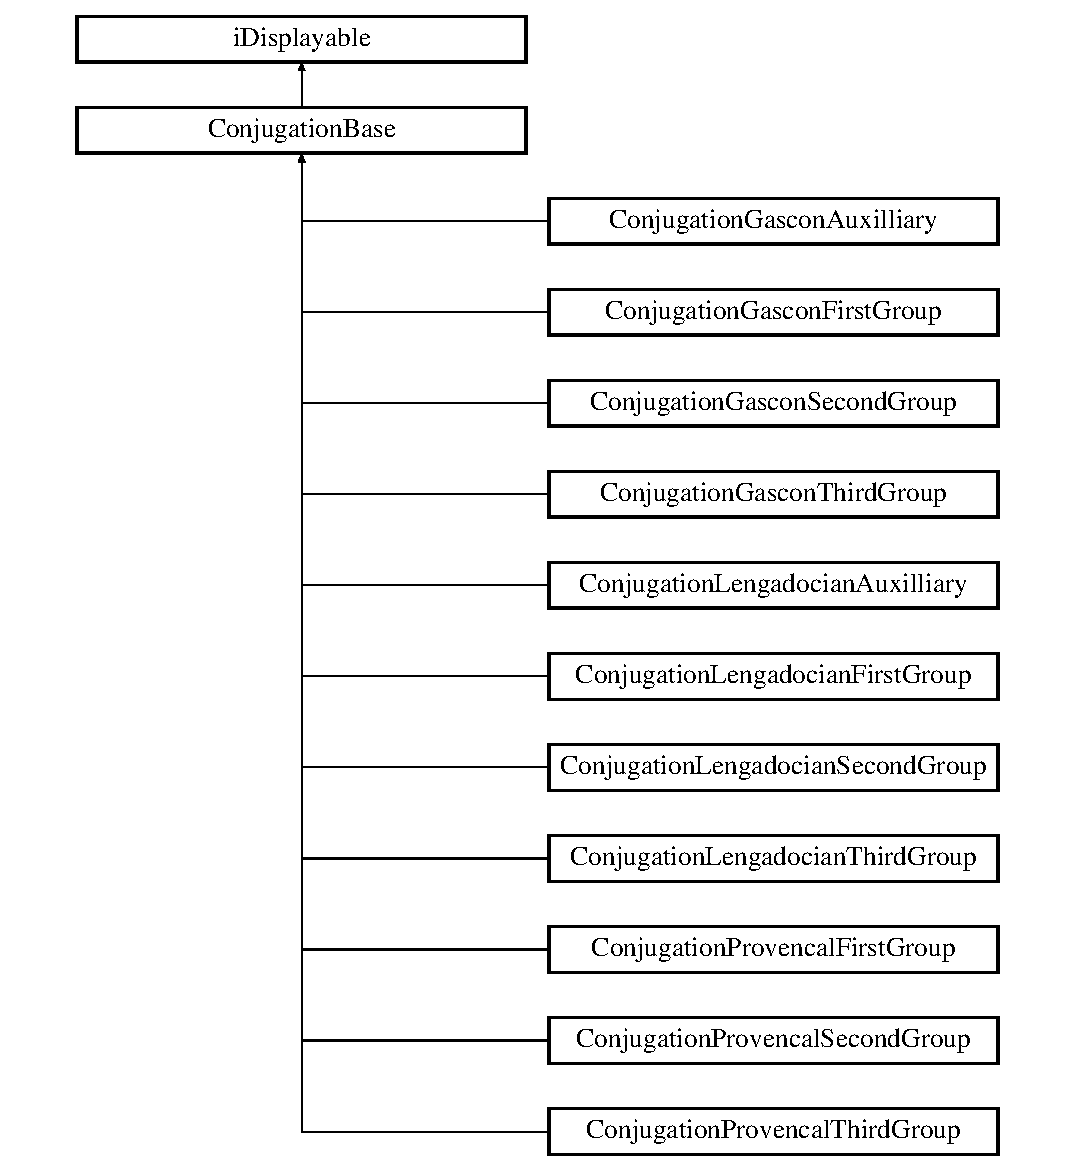
\includegraphics[height=12.000000cm]{interfaceiDisplayable}
\end{center}
\end{figure}
\subsection*{Fonctions membres publiques}
\begin{DoxyCompactItemize}
\item 
\hypertarget{interfaceiDisplayable_a0264fd455c876e897f754cf85f1681ca}{}\label{interfaceiDisplayable_a0264fd455c876e897f754cf85f1681ca} 
{\bfseries display} ()
\end{DoxyCompactItemize}


La documentation de cette interface a été générée à partir du fichier suivant \+:\begin{DoxyCompactItemize}
\item 
php/includes/\hyperlink{iDisplayable_8inc}{i\+Displayable.\+inc}\end{DoxyCompactItemize}

\chapter{Documentation des fichiers}
\hypertarget{conjoc__debug__webForm_8inc}{}\section{Référence du fichier conjoc\+\_\+debug\+\_\+web\+Form.\+inc}
\label{conjoc__debug__webForm_8inc}\index{conjoc\+\_\+debug\+\_\+web\+Form.\+inc@{conjoc\+\_\+debug\+\_\+web\+Form.\+inc}}
\subsection*{Fonctions}
\begin{DoxyCompactItemize}
\item 
\hyperlink{conjoc__debug__webForm_8inc_aafe244ee66a2c6e333d48efccec9164f}{ajax\+\_\+debug\+\_\+verb\+\_\+autocomplete} (\$form, \&\$form\+\_\+state)
\item 
\hyperlink{conjoc__debug__webForm_8inc_aedd67c4b770b58826708010ce4ef7ac7}{ajax\+\_\+debug\+\_\+verb\+\_\+autocomplete\+\_\+callback} (\$string=\char`\"{}\char`\"{})
\item 
\hypertarget{conjoc__debug__webForm_8inc_af6a94ce95f29fca17e5a3fb82855e835}{}\label{conjoc__debug__webForm_8inc_af6a94ce95f29fca17e5a3fb82855e835} 
{\bfseries debug\+\_\+\+T\+E\+I\+\_\+submit} (\$form, \&\$form\+\_\+state)
\item 
\hypertarget{conjoc__debug__webForm_8inc_a11d1063e5c7b2bf2e290639c78266d71}{}\label{conjoc__debug__webForm_8inc_a11d1063e5c7b2bf2e290639c78266d71} 
{\bfseries search\+\_\+submit} (\$form, \&\$form\+\_\+state)
\end{DoxyCompactItemize}


\subsection{Description détaillée}
conjoc\+\_\+debug\+\_\+verb\+Form.\+inc 

\subsection{Documentation des fonctions}
\hypertarget{conjoc__debug__webForm_8inc_aafe244ee66a2c6e333d48efccec9164f}{}\label{conjoc__debug__webForm_8inc_aafe244ee66a2c6e333d48efccec9164f} 
\index{conjoc\+\_\+debug\+\_\+web\+Form.\+inc@{conjoc\+\_\+debug\+\_\+web\+Form.\+inc}!ajax\+\_\+debug\+\_\+verb\+\_\+autocomplete@{ajax\+\_\+debug\+\_\+verb\+\_\+autocomplete}}
\index{ajax\+\_\+debug\+\_\+verb\+\_\+autocomplete@{ajax\+\_\+debug\+\_\+verb\+\_\+autocomplete}!conjoc\+\_\+debug\+\_\+web\+Form.\+inc@{conjoc\+\_\+debug\+\_\+web\+Form.\+inc}}
\subsubsection{\texorpdfstring{ajax\+\_\+debug\+\_\+verb\+\_\+autocomplete()}{ajax\_debug\_verb\_autocomplete()}}
{\footnotesize\ttfamily ajax\+\_\+debug\+\_\+verb\+\_\+autocomplete (\begin{DoxyParamCaption}\item[{}]{\$form,  }\item[{\&}]{\$form\+\_\+state }\end{DoxyParamCaption})}

D E B U G D E B U G D E B U G \hypertarget{conjoc__debug__webForm_8inc_aedd67c4b770b58826708010ce4ef7ac7}{}\label{conjoc__debug__webForm_8inc_aedd67c4b770b58826708010ce4ef7ac7} 
\index{conjoc\+\_\+debug\+\_\+web\+Form.\+inc@{conjoc\+\_\+debug\+\_\+web\+Form.\+inc}!ajax\+\_\+debug\+\_\+verb\+\_\+autocomplete\+\_\+callback@{ajax\+\_\+debug\+\_\+verb\+\_\+autocomplete\+\_\+callback}}
\index{ajax\+\_\+debug\+\_\+verb\+\_\+autocomplete\+\_\+callback@{ajax\+\_\+debug\+\_\+verb\+\_\+autocomplete\+\_\+callback}!conjoc\+\_\+debug\+\_\+web\+Form.\+inc@{conjoc\+\_\+debug\+\_\+web\+Form.\+inc}}
\subsubsection{\texorpdfstring{ajax\+\_\+debug\+\_\+verb\+\_\+autocomplete\+\_\+callback()}{ajax\_debug\_verb\_autocomplete\_callback()}}
{\footnotesize\ttfamily ajax\+\_\+debug\+\_\+verb\+\_\+autocomplete\+\_\+callback (\begin{DoxyParamCaption}\item[{}]{\$string = {\ttfamily \char`\"{}\char`\"{}} }\end{DoxyParamCaption})}


\begin{DoxyParams}[1]{Paramètres}
string & {\em \$string} & The string that will be searched. \\
\hline
\end{DoxyParams}

\hypertarget{conjoc__gascon__webForm_8inc}{}\section{Référence du fichier conjoc\+\_\+gascon\+\_\+web\+Form.\+inc}
\label{conjoc__gascon__webForm_8inc}\index{conjoc\+\_\+gascon\+\_\+web\+Form.\+inc@{conjoc\+\_\+gascon\+\_\+web\+Form.\+inc}}
\subsection*{Fonctions}
\begin{DoxyCompactItemize}
\item 
\hyperlink{conjoc__gascon__webForm_8inc_a28516e435edf21d85ed77091d71f5d6b}{ajax\+\_\+gascon\+\_\+verb\+\_\+autocomplete} (\$form, \&\$form\+\_\+state)
\item 
\hypertarget{conjoc__gascon__webForm_8inc_a332dbb7ab0a2190165164326af8cc7f1}{}\label{conjoc__gascon__webForm_8inc_a332dbb7ab0a2190165164326af8cc7f1} 
{\bfseries ajax\+\_\+gascon\+\_\+verb\+\_\+autocomplete\+\_\+submit} (\$form, \&\$form\+\_\+state)
\item 
\hypertarget{conjoc__gascon__webForm_8inc_aeae9bd30b3fa7e4a9edf10587db73c23}{}\label{conjoc__gascon__webForm_8inc_aeae9bd30b3fa7e4a9edf10587db73c23} 
{\bfseries gascon\+\_\+\+T\+E\+I\+\_\+submit} (\$form, \&\$form\+\_\+state)
\item 
\hyperlink{conjoc__gascon__webForm_8inc_a1be8e9edb4dcdb19c5b5bb88b48c5980}{ajax\+\_\+gascon\+\_\+verb\+\_\+autocomplete\+\_\+callback} (\$string=\char`\"{}\char`\"{})
\end{DoxyCompactItemize}


\subsection{Description détaillée}
conjoc\+\_\+gascon\+\_\+verb\+Form.\+inc 

\subsection{Documentation des fonctions}
\hypertarget{conjoc__gascon__webForm_8inc_a28516e435edf21d85ed77091d71f5d6b}{}\label{conjoc__gascon__webForm_8inc_a28516e435edf21d85ed77091d71f5d6b} 
\index{conjoc\+\_\+gascon\+\_\+web\+Form.\+inc@{conjoc\+\_\+gascon\+\_\+web\+Form.\+inc}!ajax\+\_\+gascon\+\_\+verb\+\_\+autocomplete@{ajax\+\_\+gascon\+\_\+verb\+\_\+autocomplete}}
\index{ajax\+\_\+gascon\+\_\+verb\+\_\+autocomplete@{ajax\+\_\+gascon\+\_\+verb\+\_\+autocomplete}!conjoc\+\_\+gascon\+\_\+web\+Form.\+inc@{conjoc\+\_\+gascon\+\_\+web\+Form.\+inc}}
\subsubsection{\texorpdfstring{ajax\+\_\+gascon\+\_\+verb\+\_\+autocomplete()}{ajax\_gascon\_verb\_autocomplete()}}
{\footnotesize\ttfamily ajax\+\_\+gascon\+\_\+verb\+\_\+autocomplete (\begin{DoxyParamCaption}\item[{}]{\$form,  }\item[{\&}]{\$form\+\_\+state }\end{DoxyParamCaption})}

G A S C O N G A S C O N G A S C O N \hypertarget{conjoc__gascon__webForm_8inc_a1be8e9edb4dcdb19c5b5bb88b48c5980}{}\label{conjoc__gascon__webForm_8inc_a1be8e9edb4dcdb19c5b5bb88b48c5980} 
\index{conjoc\+\_\+gascon\+\_\+web\+Form.\+inc@{conjoc\+\_\+gascon\+\_\+web\+Form.\+inc}!ajax\+\_\+gascon\+\_\+verb\+\_\+autocomplete\+\_\+callback@{ajax\+\_\+gascon\+\_\+verb\+\_\+autocomplete\+\_\+callback}}
\index{ajax\+\_\+gascon\+\_\+verb\+\_\+autocomplete\+\_\+callback@{ajax\+\_\+gascon\+\_\+verb\+\_\+autocomplete\+\_\+callback}!conjoc\+\_\+gascon\+\_\+web\+Form.\+inc@{conjoc\+\_\+gascon\+\_\+web\+Form.\+inc}}
\subsubsection{\texorpdfstring{ajax\+\_\+gascon\+\_\+verb\+\_\+autocomplete\+\_\+callback()}{ajax\_gascon\_verb\_autocomplete\_callback()}}
{\footnotesize\ttfamily ajax\+\_\+gascon\+\_\+verb\+\_\+autocomplete\+\_\+callback (\begin{DoxyParamCaption}\item[{}]{\$string = {\ttfamily \char`\"{}\char`\"{}} }\end{DoxyParamCaption})}


\begin{DoxyParams}[1]{Paramètres}
string & {\em \$string} & The string that will be searched. \\
\hline
\end{DoxyParams}

\hypertarget{conjoc__lengadocian__webForm_8inc}{}\section{Référence du fichier conjoc\+\_\+lengadocian\+\_\+web\+Form.\+inc}
\label{conjoc__lengadocian__webForm_8inc}\index{conjoc\+\_\+lengadocian\+\_\+web\+Form.\+inc@{conjoc\+\_\+lengadocian\+\_\+web\+Form.\+inc}}
\subsection*{Fonctions}
\begin{DoxyCompactItemize}
\item 
\hyperlink{conjoc__lengadocian__webForm_8inc_a9c7725a828c1a44761bc51fe7a346215}{tei\+\_\+export\+\_\+lengadocian\+\_\+all} (\$form, \&\$form\+\_\+state)
\item 
\hypertarget{conjoc__lengadocian__webForm_8inc_a465cce16b0d09f364ccb546c46c82306}{}\label{conjoc__lengadocian__webForm_8inc_a465cce16b0d09f364ccb546c46c82306} 
{\bfseries indexation\+\_\+lengadocian\+\_\+all} (\$form, \&\$form\+\_\+state)
\item 
\hypertarget{conjoc__lengadocian__webForm_8inc_a3f7b0b4a8f4301190850532d5488c54a}{}\label{conjoc__lengadocian__webForm_8inc_a3f7b0b4a8f4301190850532d5488c54a} 
{\bfseries indexation\+\_\+searchform} (\$form, \&\$form\+\_\+state)
\item 
\hypertarget{conjoc__lengadocian__webForm_8inc_a95265729a90a0b79d7d98483fce78880}{}\label{conjoc__lengadocian__webForm_8inc_a95265729a90a0b79d7d98483fce78880} 
{\bfseries ajax\+\_\+lengadocian\+\_\+verb\+\_\+autocomplete} (\$form, \&\$form\+\_\+state)
\item 
\hypertarget{conjoc__lengadocian__webForm_8inc_a2206d720f533b7b1afa6ac0568e740ef}{}\label{conjoc__lengadocian__webForm_8inc_a2206d720f533b7b1afa6ac0568e740ef} 
{\bfseries ajax\+\_\+lengadocian\+\_\+verb\+\_\+autocomplete\+\_\+submit} (\$form, \&\$form\+\_\+state)
\item 
\hyperlink{conjoc__lengadocian__webForm_8inc_a26cea88ddc504d14492fa9fd58a060b4}{ajax\+\_\+lengadocian\+\_\+verb\+\_\+autocomplete\+\_\+callback} (\$string=\char`\"{}\char`\"{})
\item 
\hypertarget{conjoc__lengadocian__webForm_8inc_a704a4de756f6a38064970e97d4a2bc6c}{}\label{conjoc__lengadocian__webForm_8inc_a704a4de756f6a38064970e97d4a2bc6c} 
{\bfseries lengadocian\+\_\+\+T\+E\+I\+\_\+submit} (\$form, \&\$form\+\_\+state)
\item 
\hypertarget{conjoc__lengadocian__webForm_8inc_ad10d751f3d75ba568eb1f41bd43fcc94}{}\label{conjoc__lengadocian__webForm_8inc_ad10d751f3d75ba568eb1f41bd43fcc94} 
{\bfseries conjoc\+\_\+form\+\_\+submit} (\$form, \&\$form\+\_\+state)
\item 
\hyperlink{conjoc__lengadocian__webForm_8inc_a378d4601a46c698692d26cb301470598}{verb\+\_\+autocomplete\+\_\+indexation\+\_\+callback} (\$string=\char`\"{}\char`\"{})
\item 
\hypertarget{conjoc__lengadocian__webForm_8inc_a5e7b0be9cab73b5b2be66499afd0edc5}{}\label{conjoc__lengadocian__webForm_8inc_a5e7b0be9cab73b5b2be66499afd0edc5} 
{\bfseries verb\+\_\+autocomplete\+\_\+indexation\+\_\+submit} (\$form, \&\$form\+\_\+state)
\item 
\hypertarget{conjoc__lengadocian__webForm_8inc_afecc813b5558b906fe6cc9adb1419c35}{}\label{conjoc__lengadocian__webForm_8inc_afecc813b5558b906fe6cc9adb1419c35} 
{\bfseries process\+\_\+\+U\+R\+L\+\_\+arguments} (\$content=N\+U\+LL, \$arg1=N\+U\+LL, \$arg2=N\+U\+LL)
\item 
\hyperlink{conjoc__lengadocian__webForm_8inc_a4ffe99e612db8d794975a33aefb781f7}{\+\_\+lengadocian\+\_\+menu\+\_\+page} (\$content=N\+U\+LL, \$arg1=N\+U\+LL, \$arg2=N\+U\+LL)
\end{DoxyCompactItemize}


\subsection{Description détaillée}
conjoc\+\_\+lengadocian\+\_\+verb\+Form.\+inc

Demonstrates usage of the Form A\+PI\textquotesingle{}s autocomplete features.

This file provides three examples in increasing complexity\+:
\begin{DoxyItemize}
\item A simple username autocomplete (usernames are unique, so little effort is required)
\item A node title autocomplete (titles are not unique, so we have to find the nid and stash it in the field)
\item A username autocomplete that updates a node title autocomplete with a changed \#autocomplete\+\_\+path so that the \#autocomplete\+\_\+path can have context (the username to use in the search). 
\end{DoxyItemize}

\subsection{Documentation des fonctions}
\hypertarget{conjoc__lengadocian__webForm_8inc_a4ffe99e612db8d794975a33aefb781f7}{}\label{conjoc__lengadocian__webForm_8inc_a4ffe99e612db8d794975a33aefb781f7} 
\index{conjoc\+\_\+lengadocian\+\_\+web\+Form.\+inc@{conjoc\+\_\+lengadocian\+\_\+web\+Form.\+inc}!\+\_\+lengadocian\+\_\+menu\+\_\+page@{\+\_\+lengadocian\+\_\+menu\+\_\+page}}
\index{\+\_\+lengadocian\+\_\+menu\+\_\+page@{\+\_\+lengadocian\+\_\+menu\+\_\+page}!conjoc\+\_\+lengadocian\+\_\+web\+Form.\+inc@{conjoc\+\_\+lengadocian\+\_\+web\+Form.\+inc}}
\subsubsection{\texorpdfstring{\+\_\+lengadocian\+\_\+menu\+\_\+page()}{\_lengadocian\_menu\_page()}}
{\footnotesize\ttfamily \+\_\+lengadocian\+\_\+menu\+\_\+page (\begin{DoxyParamCaption}\item[{}]{\$content = {\ttfamily NULL},  }\item[{}]{\$arg1 = {\ttfamily NULL},  }\item[{}]{\$arg2 = {\ttfamily NULL} }\end{DoxyParamCaption})}

Page callback for use with most of the menu entries.

The arguments it receives determine what it outputs.


\begin{DoxyParams}[1]{Paramètres}
string & {\em \$content} & The base content to output. \\
\hline
string & {\em \$arg1} & First additional argument from the path used to access the menu \\
\hline
string & {\em \$arg2} & Second additional argument. \\
\hline
\end{DoxyParams}
\hypertarget{conjoc__lengadocian__webForm_8inc_a26cea88ddc504d14492fa9fd58a060b4}{}\label{conjoc__lengadocian__webForm_8inc_a26cea88ddc504d14492fa9fd58a060b4} 
\index{conjoc\+\_\+lengadocian\+\_\+web\+Form.\+inc@{conjoc\+\_\+lengadocian\+\_\+web\+Form.\+inc}!ajax\+\_\+lengadocian\+\_\+verb\+\_\+autocomplete\+\_\+callback@{ajax\+\_\+lengadocian\+\_\+verb\+\_\+autocomplete\+\_\+callback}}
\index{ajax\+\_\+lengadocian\+\_\+verb\+\_\+autocomplete\+\_\+callback@{ajax\+\_\+lengadocian\+\_\+verb\+\_\+autocomplete\+\_\+callback}!conjoc\+\_\+lengadocian\+\_\+web\+Form.\+inc@{conjoc\+\_\+lengadocian\+\_\+web\+Form.\+inc}}
\subsubsection{\texorpdfstring{ajax\+\_\+lengadocian\+\_\+verb\+\_\+autocomplete\+\_\+callback()}{ajax\_lengadocian\_verb\_autocomplete\_callback()}}
{\footnotesize\ttfamily ajax\+\_\+lengadocian\+\_\+verb\+\_\+autocomplete\+\_\+callback (\begin{DoxyParamCaption}\item[{}]{\$string = {\ttfamily \char`\"{}\char`\"{}} }\end{DoxyParamCaption})}


\begin{DoxyParams}[1]{Paramètres}
string & {\em \$string} & The string that will be searched. \\
\hline
\end{DoxyParams}
\hypertarget{conjoc__lengadocian__webForm_8inc_a9c7725a828c1a44761bc51fe7a346215}{}\label{conjoc__lengadocian__webForm_8inc_a9c7725a828c1a44761bc51fe7a346215} 
\index{conjoc\+\_\+lengadocian\+\_\+web\+Form.\+inc@{conjoc\+\_\+lengadocian\+\_\+web\+Form.\+inc}!tei\+\_\+export\+\_\+lengadocian\+\_\+all@{tei\+\_\+export\+\_\+lengadocian\+\_\+all}}
\index{tei\+\_\+export\+\_\+lengadocian\+\_\+all@{tei\+\_\+export\+\_\+lengadocian\+\_\+all}!conjoc\+\_\+lengadocian\+\_\+web\+Form.\+inc@{conjoc\+\_\+lengadocian\+\_\+web\+Form.\+inc}}
\subsubsection{\texorpdfstring{tei\+\_\+export\+\_\+lengadocian\+\_\+all()}{tei\_export\_lengadocian\_all()}}
{\footnotesize\ttfamily tei\+\_\+export\+\_\+lengadocian\+\_\+all (\begin{DoxyParamCaption}\item[{}]{\$form,  }\item[{\&}]{\$form\+\_\+state }\end{DoxyParamCaption})}

L\+E\+N\+G\+A\+D\+O\+C\+I\+AN \hypertarget{conjoc__lengadocian__webForm_8inc_a378d4601a46c698692d26cb301470598}{}\label{conjoc__lengadocian__webForm_8inc_a378d4601a46c698692d26cb301470598} 
\index{conjoc\+\_\+lengadocian\+\_\+web\+Form.\+inc@{conjoc\+\_\+lengadocian\+\_\+web\+Form.\+inc}!verb\+\_\+autocomplete\+\_\+indexation\+\_\+callback@{verb\+\_\+autocomplete\+\_\+indexation\+\_\+callback}}
\index{verb\+\_\+autocomplete\+\_\+indexation\+\_\+callback@{verb\+\_\+autocomplete\+\_\+indexation\+\_\+callback}!conjoc\+\_\+lengadocian\+\_\+web\+Form.\+inc@{conjoc\+\_\+lengadocian\+\_\+web\+Form.\+inc}}
\subsubsection{\texorpdfstring{verb\+\_\+autocomplete\+\_\+indexation\+\_\+callback()}{verb\_autocomplete\_indexation\_callback()}}
{\footnotesize\ttfamily verb\+\_\+autocomplete\+\_\+indexation\+\_\+callback (\begin{DoxyParamCaption}\item[{}]{\$string = {\ttfamily \char`\"{}\char`\"{}} }\end{DoxyParamCaption})}


\begin{DoxyParams}[1]{Paramètres}
string & {\em \$string} & The string that will be searched. \\
\hline
\end{DoxyParams}

\hypertarget{conjoc__provencal__webForm_8inc}{}\section{Référence du fichier conjoc\+\_\+provencal\+\_\+web\+Form.\+inc}
\label{conjoc__provencal__webForm_8inc}\index{conjoc\+\_\+provencal\+\_\+web\+Form.\+inc@{conjoc\+\_\+provencal\+\_\+web\+Form.\+inc}}
\subsection*{Fonctions}
\begin{DoxyCompactItemize}
\item 
\hyperlink{conjoc__provencal__webForm_8inc_aac31f536bfd83a81f1ea012f5ecdc9ad}{ajax\+\_\+provencal\+\_\+verb\+\_\+autocomplete} (\$form, \&\$form\+\_\+state)
\item 
\hyperlink{conjoc__provencal__webForm_8inc_a2f2da1c5cc327e80252b73dd250aa363}{ajax\+\_\+provencal\+\_\+verb\+\_\+autocomplete\+\_\+callback} (\$string=\char`\"{}\char`\"{})
\item 
\hypertarget{conjoc__provencal__webForm_8inc_a8e95bdf8c2d2a450e6485d589788aa83}{}\label{conjoc__provencal__webForm_8inc_a8e95bdf8c2d2a450e6485d589788aa83} 
{\bfseries conjoc\+\_\+get\+Random\+Provencal\+Verb} ()
\end{DoxyCompactItemize}


\subsection{Description détaillée}
conjoc\+\_\+provencal\+\_\+verb\+Form.\+inc 

\subsection{Documentation des fonctions}
\hypertarget{conjoc__provencal__webForm_8inc_aac31f536bfd83a81f1ea012f5ecdc9ad}{}\label{conjoc__provencal__webForm_8inc_aac31f536bfd83a81f1ea012f5ecdc9ad} 
\index{conjoc\+\_\+provencal\+\_\+web\+Form.\+inc@{conjoc\+\_\+provencal\+\_\+web\+Form.\+inc}!ajax\+\_\+provencal\+\_\+verb\+\_\+autocomplete@{ajax\+\_\+provencal\+\_\+verb\+\_\+autocomplete}}
\index{ajax\+\_\+provencal\+\_\+verb\+\_\+autocomplete@{ajax\+\_\+provencal\+\_\+verb\+\_\+autocomplete}!conjoc\+\_\+provencal\+\_\+web\+Form.\+inc@{conjoc\+\_\+provencal\+\_\+web\+Form.\+inc}}
\subsubsection{\texorpdfstring{ajax\+\_\+provencal\+\_\+verb\+\_\+autocomplete()}{ajax\_provencal\_verb\_autocomplete()}}
{\footnotesize\ttfamily ajax\+\_\+provencal\+\_\+verb\+\_\+autocomplete (\begin{DoxyParamCaption}\item[{}]{\$form,  }\item[{\&}]{\$form\+\_\+state }\end{DoxyParamCaption})}

P R O V E N C A L P R O V E N C A L P R O V E N C A L \hypertarget{conjoc__provencal__webForm_8inc_a2f2da1c5cc327e80252b73dd250aa363}{}\label{conjoc__provencal__webForm_8inc_a2f2da1c5cc327e80252b73dd250aa363} 
\index{conjoc\+\_\+provencal\+\_\+web\+Form.\+inc@{conjoc\+\_\+provencal\+\_\+web\+Form.\+inc}!ajax\+\_\+provencal\+\_\+verb\+\_\+autocomplete\+\_\+callback@{ajax\+\_\+provencal\+\_\+verb\+\_\+autocomplete\+\_\+callback}}
\index{ajax\+\_\+provencal\+\_\+verb\+\_\+autocomplete\+\_\+callback@{ajax\+\_\+provencal\+\_\+verb\+\_\+autocomplete\+\_\+callback}!conjoc\+\_\+provencal\+\_\+web\+Form.\+inc@{conjoc\+\_\+provencal\+\_\+web\+Form.\+inc}}
\subsubsection{\texorpdfstring{ajax\+\_\+provencal\+\_\+verb\+\_\+autocomplete\+\_\+callback()}{ajax\_provencal\_verb\_autocomplete\_callback()}}
{\footnotesize\ttfamily ajax\+\_\+provencal\+\_\+verb\+\_\+autocomplete\+\_\+callback (\begin{DoxyParamCaption}\item[{}]{\$string = {\ttfamily \char`\"{}\char`\"{}} }\end{DoxyParamCaption})}


\begin{DoxyParams}[1]{Paramètres}
string & {\em \$string} & The string that will be searched. \\
\hline
\end{DoxyParams}

\hypertarget{conjoc__webForm_8inc}{}\section{Référence du fichier conjoc\+\_\+web\+Form.\+inc}
\label{conjoc__webForm_8inc}\index{conjoc\+\_\+web\+Form.\+inc@{conjoc\+\_\+web\+Form.\+inc}}
\subsection*{Fonctions}
\begin{DoxyCompactItemize}
\item 
\hyperlink{conjoc__webForm_8inc_a9c7725a828c1a44761bc51fe7a346215}{tei\+\_\+export\+\_\+lengadocian\+\_\+all} (\$form, \&\$form\+\_\+state)
\item 
\hypertarget{conjoc__webForm_8inc_a465cce16b0d09f364ccb546c46c82306}{}\label{conjoc__webForm_8inc_a465cce16b0d09f364ccb546c46c82306} 
{\bfseries indexation\+\_\+lengadocian\+\_\+all} (\$form, \&\$form\+\_\+state)
\item 
\hypertarget{conjoc__webForm_8inc_a3698c970fd73cda200a3a459dc50beec}{}\label{conjoc__webForm_8inc_a3698c970fd73cda200a3a459dc50beec} 
{\bfseries ajax\+\_\+conjoc\+\_\+verb\+\_\+autocomplete} (\$form, \&\$form\+\_\+state)
\item 
\hyperlink{conjoc__webForm_8inc_a5ea54e98ecadf55b7fe917fe6237a52e}{ajax\+\_\+conjoc\+\_\+verb\+\_\+autocomplete\+\_\+callback} (\$string=\char`\"{}\char`\"{})
\item 
\hyperlink{conjoc__webForm_8inc_add934c4187ded056db9c8369764a51ed}{ajax\+\_\+conjoc\+\_\+verb\+\_\+autocomplete\+\_\+submit} (\$form, \&\$form\+\_\+state)
\item 
\hyperlink{conjoc__webForm_8inc_ae85a92c4f091005289a97fb20b8762ef}{ajax\+\_\+conjoc\+\_\+verb\+\_\+autocomplete\+\_\+validate} (\$form, \&\$form\+\_\+state)
\item 
\hypertarget{conjoc__webForm_8inc_aacc782a067b5e8fdaeca34be9a282c61}{}\label{conjoc__webForm_8inc_aacc782a067b5e8fdaeca34be9a282c61} 
{\bfseries conjoc\+\_\+get\+Random\+Lengadocian\+Verb} ()
\item 
\hypertarget{conjoc__webForm_8inc_aab99a7a60692cf7228d4a79924c32cb2}{}\label{conjoc__webForm_8inc_aab99a7a60692cf7228d4a79924c32cb2} 
{\bfseries conjugador\+\_\+l} (\$verb=N\+U\+LL, \$action=N\+U\+LL)
\item 
\hypertarget{conjoc__webForm_8inc_a5d341264c049e9bda5fd2d0acce4dfd7}{}\label{conjoc__webForm_8inc_a5d341264c049e9bda5fd2d0acce4dfd7} 
{\bfseries conjugador\+\_\+conjugate} (\$verb, \$model)
\item 
\hypertarget{conjoc__webForm_8inc_a16562f736e2ff741407adb1ceb3c9170}{}\label{conjoc__webForm_8inc_a16562f736e2ff741407adb1ceb3c9170} 
{\bfseries conjugador\+\_\+displaynotes} (\$nummodel)
\item 
\hypertarget{conjoc__webForm_8inc_ac41ee7cf6ccd6dd46de8112c7c315cfe}{}\label{conjoc__webForm_8inc_ac41ee7cf6ccd6dd46de8112c7c315cfe} 
{\bfseries conjugador\+\_\+display\+Singles} ()
\item 
\hypertarget{conjoc__webForm_8inc_adfb69460570fdffecec436447f5ed729}{}\label{conjoc__webForm_8inc_adfb69460570fdffecec436447f5ed729} 
{\bfseries conjugador\+\_\+display\+Top20} (\$verb\+Current)
\item 
\hypertarget{conjoc__webForm_8inc_a64885b968e081840d6a10adc2a38db9e}{}\label{conjoc__webForm_8inc_a64885b968e081840d6a10adc2a38db9e} 
{\bfseries conjugador\+\_\+display\+Others\+In\+Model} (\$verb)
\item 
\hypertarget{conjoc__webForm_8inc_ac96a30f96cb3957ed4ac47c4eb40df10}{}\label{conjoc__webForm_8inc_ac96a30f96cb3957ed4ac47c4eb40df10} 
{\bfseries conjugador\+\_\+count\+Others\+In\+Model} (\$verb)
\item 
\hypertarget{conjoc__webForm_8inc_a1bfbce593ac5c763b1542fa713249aa3}{}\label{conjoc__webForm_8inc_a1bfbce593ac5c763b1542fa713249aa3} 
{\bfseries conjugador\+\_\+display\+Usuals} ()
\item 
\hypertarget{conjoc__webForm_8inc_a9ab9dfc2c3015a0855c27f37812bb897}{}\label{conjoc__webForm_8inc_a9ab9dfc2c3015a0855c27f37812bb897} 
{\bfseries conjugador\+\_\+get\+Top20} ()
\item 
\hypertarget{conjoc__webForm_8inc_a90ac7751a59eefed3b3576f1cedb016f}{}\label{conjoc__webForm_8inc_a90ac7751a59eefed3b3576f1cedb016f} 
{\bfseries conjugador\+\_\+get\+Others\+In\+Model} (\$verb)
\end{DoxyCompactItemize}


\subsection{Description détaillée}
conjoc\+\_\+verb\+Form.\+inc

Demonstrates usage of the Form A\+PI\textquotesingle{}s autocomplete features.

This file provides three examples in increasing complexity\+:
\begin{DoxyItemize}
\item A simple username autocomplete (usernames are unique, so little effort is required)
\item A node title autocomplete (titles are not unique, so we have to find the nid and stash it in the field)
\item A username autocomplete that updates a node title autocomplete with a changed \#autocomplete\+\_\+path so that the \#autocomplete\+\_\+path can have context (the username to use in the search). 
\end{DoxyItemize}

\subsection{Documentation des fonctions}
\hypertarget{conjoc__webForm_8inc_a5ea54e98ecadf55b7fe917fe6237a52e}{}\label{conjoc__webForm_8inc_a5ea54e98ecadf55b7fe917fe6237a52e} 
\index{conjoc\+\_\+web\+Form.\+inc@{conjoc\+\_\+web\+Form.\+inc}!ajax\+\_\+conjoc\+\_\+verb\+\_\+autocomplete\+\_\+callback@{ajax\+\_\+conjoc\+\_\+verb\+\_\+autocomplete\+\_\+callback}}
\index{ajax\+\_\+conjoc\+\_\+verb\+\_\+autocomplete\+\_\+callback@{ajax\+\_\+conjoc\+\_\+verb\+\_\+autocomplete\+\_\+callback}!conjoc\+\_\+web\+Form.\+inc@{conjoc\+\_\+web\+Form.\+inc}}
\subsubsection{\texorpdfstring{ajax\+\_\+conjoc\+\_\+verb\+\_\+autocomplete\+\_\+callback()}{ajax\_conjoc\_verb\_autocomplete\_callback()}}
{\footnotesize\ttfamily ajax\+\_\+conjoc\+\_\+verb\+\_\+autocomplete\+\_\+callback (\begin{DoxyParamCaption}\item[{}]{\$string = {\ttfamily \char`\"{}\char`\"{}} }\end{DoxyParamCaption})}


\begin{DoxyParams}[1]{Paramètres}
string & {\em \$string} & The string that will be searched. \\
\hline
\end{DoxyParams}
\hypertarget{conjoc__webForm_8inc_add934c4187ded056db9c8369764a51ed}{}\label{conjoc__webForm_8inc_add934c4187ded056db9c8369764a51ed} 
\index{conjoc\+\_\+web\+Form.\+inc@{conjoc\+\_\+web\+Form.\+inc}!ajax\+\_\+conjoc\+\_\+verb\+\_\+autocomplete\+\_\+submit@{ajax\+\_\+conjoc\+\_\+verb\+\_\+autocomplete\+\_\+submit}}
\index{ajax\+\_\+conjoc\+\_\+verb\+\_\+autocomplete\+\_\+submit@{ajax\+\_\+conjoc\+\_\+verb\+\_\+autocomplete\+\_\+submit}!conjoc\+\_\+web\+Form.\+inc@{conjoc\+\_\+web\+Form.\+inc}}
\subsubsection{\texorpdfstring{ajax\+\_\+conjoc\+\_\+verb\+\_\+autocomplete\+\_\+submit()}{ajax\_conjoc\_verb\_autocomplete\_submit()}}
{\footnotesize\ttfamily ajax\+\_\+conjoc\+\_\+verb\+\_\+autocomplete\+\_\+submit (\begin{DoxyParamCaption}\item[{}]{\$form,  }\item[{\&}]{\$form\+\_\+state }\end{DoxyParamCaption})}

Submit handler for node lookup unique autocomplete example.

Here the nid has already been placed in \$form\+\_\+state\mbox{[}\textquotesingle{}values\textquotesingle{}\mbox{]}\mbox{[}\textquotesingle{}node\textquotesingle{}\mbox{]} by the validation handler.


\begin{DoxyParams}[1]{Paramètres}
array & {\em \$form} & Form A\+PI form. \\
\hline
array & {\em \$form\+\_\+state} & Form A\+PI form state.\\
\hline
\end{DoxyParams}
\begin{DoxyReturn}{Renvoie}
array Form A\+PI array. 
\end{DoxyReturn}
\hypertarget{conjoc__webForm_8inc_ae85a92c4f091005289a97fb20b8762ef}{}\label{conjoc__webForm_8inc_ae85a92c4f091005289a97fb20b8762ef} 
\index{conjoc\+\_\+web\+Form.\+inc@{conjoc\+\_\+web\+Form.\+inc}!ajax\+\_\+conjoc\+\_\+verb\+\_\+autocomplete\+\_\+validate@{ajax\+\_\+conjoc\+\_\+verb\+\_\+autocomplete\+\_\+validate}}
\index{ajax\+\_\+conjoc\+\_\+verb\+\_\+autocomplete\+\_\+validate@{ajax\+\_\+conjoc\+\_\+verb\+\_\+autocomplete\+\_\+validate}!conjoc\+\_\+web\+Form.\+inc@{conjoc\+\_\+web\+Form.\+inc}}
\subsubsection{\texorpdfstring{ajax\+\_\+conjoc\+\_\+verb\+\_\+autocomplete\+\_\+validate()}{ajax\_conjoc\_verb\_autocomplete\_validate()}}
{\footnotesize\ttfamily ajax\+\_\+conjoc\+\_\+verb\+\_\+autocomplete\+\_\+validate (\begin{DoxyParamCaption}\item[{}]{\$form,  }\item[{\&}]{\$form\+\_\+state }\end{DoxyParamCaption})}


\begin{DoxyParams}[1]{Paramètres}
array & {\em \$form} & Form A\+PI form. \\
\hline
array & {\em \$form\+\_\+state} & Form A\+PI form state. \\
\hline
\end{DoxyParams}
\hypertarget{conjoc__webForm_8inc_a9c7725a828c1a44761bc51fe7a346215}{}\label{conjoc__webForm_8inc_a9c7725a828c1a44761bc51fe7a346215} 
\index{conjoc\+\_\+web\+Form.\+inc@{conjoc\+\_\+web\+Form.\+inc}!tei\+\_\+export\+\_\+lengadocian\+\_\+all@{tei\+\_\+export\+\_\+lengadocian\+\_\+all}}
\index{tei\+\_\+export\+\_\+lengadocian\+\_\+all@{tei\+\_\+export\+\_\+lengadocian\+\_\+all}!conjoc\+\_\+web\+Form.\+inc@{conjoc\+\_\+web\+Form.\+inc}}
\subsubsection{\texorpdfstring{tei\+\_\+export\+\_\+lengadocian\+\_\+all()}{tei\_export\_lengadocian\_all()}}
{\footnotesize\ttfamily tei\+\_\+export\+\_\+lengadocian\+\_\+all (\begin{DoxyParamCaption}\item[{}]{\$form,  }\item[{\&}]{\$form\+\_\+state }\end{DoxyParamCaption})}

L E N G A D O C I A N L E N G A D O C I A N L E N G A D O C I A N 
\hypertarget{ConjugationBase_8inc}{}\section{Référence du fichier php/includes/\+Conjugation\+Base.inc}
\label{ConjugationBase_8inc}\index{php/includes/\+Conjugation\+Base.\+inc@{php/includes/\+Conjugation\+Base.\+inc}}


Base class for worker class Conjugation.  


\subsection*{Classes}
\begin{DoxyCompactItemize}
\item 
class \hyperlink{classConjugationBase}{Conjugation\+Base}
\end{DoxyCompactItemize}


\subsection{Description détaillée}
Base class for worker class Conjugation. 

\begin{DoxyAuthor}{Auteur}
Domenge Château-\/\+Annaud 
\end{DoxyAuthor}
\begin{DoxyVersion}{Version}
1.\+0 
\end{DoxyVersion}
\begin{DoxyDate}{Date}
May 2016
\end{DoxyDate}
implements everything possible and leave some abstract fonctions to be implemented by descendants. 
\hypertarget{ConjugationDataProviderBase_8inc}{}\section{Référence du fichier php/includes/\+Conjugation\+Data\+Provider\+Base.inc}
\label{ConjugationDataProviderBase_8inc}\index{php/includes/\+Conjugation\+Data\+Provider\+Base.\+inc@{php/includes/\+Conjugation\+Data\+Provider\+Base.\+inc}}


Base class for worker class Conjugation\+Data\+Provider.  


\subsection*{Classes}
\begin{DoxyCompactItemize}
\item 
class \hyperlink{classConjugationDataProviderBase}{Conjugation\+Data\+Provider\+Base}
\end{DoxyCompactItemize}


\subsection{Description détaillée}
Base class for worker class Conjugation\+Data\+Provider. 

\begin{DoxyAuthor}{Auteur}
Domenge Château-\/\+Annaud 
\end{DoxyAuthor}
\begin{DoxyVersion}{Version}
1.\+0 
\end{DoxyVersion}
\begin{DoxyDate}{Date}
May 2016
\end{DoxyDate}
this hierarchy of classes implements the data access layer in order to isolate the data persistance. 
\hypertarget{ConjugationManagerBase_8inc}{}\section{Référence du fichier php/includes/\+Conjugation\+Manager\+Base.inc}
\label{ConjugationManagerBase_8inc}\index{php/includes/\+Conjugation\+Manager\+Base.\+inc@{php/includes/\+Conjugation\+Manager\+Base.\+inc}}


abstract class that contains most of the code for all the managers of spectific dialects  


\subsection*{Classes}
\begin{DoxyCompactItemize}
\item 
class \hyperlink{classConjugationManagerBase}{Conjugation\+Manager\+Base}
\end{DoxyCompactItemize}


\subsection{Description détaillée}
abstract class that contains most of the code for all the managers of spectific dialects 

\begin{DoxyAuthor}{Auteur}
Domenge Château-\/\+Annaud 
\end{DoxyAuthor}
\begin{DoxyVersion}{Version}
1.\+0 
\end{DoxyVersion}
\begin{DoxyDate}{Date}
May 2016
\end{DoxyDate}
the manager is the central class of the framework 
\hypertarget{ConverterCSV_8inc}{}\section{Référence du fichier php/includes/\+Converter\+C\+SV.inc}
\label{ConverterCSV_8inc}\index{php/includes/\+Converter\+C\+S\+V.\+inc@{php/includes/\+Converter\+C\+S\+V.\+inc}}


converts a conjugation in C\+VS format  


\subsection*{Classes}
\begin{DoxyCompactItemize}
\item 
class \hyperlink{classConverterCSV}{Converter\+C\+SV}
\end{DoxyCompactItemize}


\subsection{Description détaillée}
converts a conjugation in C\+VS format 

\begin{DoxyAuthor}{Auteur}
Domenge Château-\/\+Annaud 
\end{DoxyAuthor}
\begin{DoxyVersion}{Version}
1.\+0 
\end{DoxyVersion}
\begin{DoxyDate}{Date}
May 2016 
\end{DoxyDate}

\hypertarget{ConverterIndexation_8inc}{}\section{Référence du fichier php/includes/\+Converter\+Indexation.inc}
\label{ConverterIndexation_8inc}\index{php/includes/\+Converter\+Indexation.\+inc@{php/includes/\+Converter\+Indexation.\+inc}}


A working implementation class to process lengadocians auxilliaries.  


\subsection*{Classes}
\begin{DoxyCompactItemize}
\item 
class \hyperlink{classConverterIndexation}{Converter\+Indexation}
\end{DoxyCompactItemize}


\subsection{Description détaillée}
A working implementation class to process lengadocians auxilliaries. 

\begin{DoxyAuthor}{Auteur}
Domenge Château-\/\+Annaud 
\end{DoxyAuthor}
\begin{DoxyVersion}{Version}
1.\+0 
\end{DoxyVersion}
\begin{DoxyDate}{Date}
May 2016 
\end{DoxyDate}

\hypertarget{ConverterLATEX_8inc}{}\section{Référence du fichier php/includes/\+Converter\+L\+A\+T\+EX.inc}
\label{ConverterLATEX_8inc}\index{php/includes/\+Converter\+L\+A\+T\+E\+X.\+inc@{php/includes/\+Converter\+L\+A\+T\+E\+X.\+inc}}


builds a pdf file with a conjugation and returns the name of the file.  


\subsection*{Classes}
\begin{DoxyCompactItemize}
\item 
class \hyperlink{classConverterLATEX}{Converter\+L\+A\+T\+EX}
\end{DoxyCompactItemize}


\subsection{Description détaillée}
builds a pdf file with a conjugation and returns the name of the file. 

\begin{DoxyAuthor}{Auteur}
Domenge Château-\/\+Annaud 
\end{DoxyAuthor}
\begin{DoxyVersion}{Version}
1.\+0 
\end{DoxyVersion}
\begin{DoxyDate}{Date}
May 2016
\end{DoxyDate}
takes a template file for La\+TeX and stuffs it with the real conjugation filling, builds a pdf file and returns the name of the file. A lot of unix commands and pdflatex are called outside of the php process. 
\hypertarget{ConverterTEI_8inc}{}\section{Référence du fichier php/includes/\+Converter\+T\+EI.inc}
\label{ConverterTEI_8inc}\index{php/includes/\+Converter\+T\+E\+I.\+inc@{php/includes/\+Converter\+T\+E\+I.\+inc}}


converts a conjugation in full T\+E\+I/\+X\+ML format (T\+E\+XT E\+N\+C\+O\+D\+I\+NG I\+N\+I\+T\+I\+A\+T\+I\+VE)  


\subsection*{Classes}
\begin{DoxyCompactItemize}
\item 
class \hyperlink{classConverterTEI}{Converter\+T\+EI}
\end{DoxyCompactItemize}


\subsection{Description détaillée}
converts a conjugation in full T\+E\+I/\+X\+ML format (T\+E\+XT E\+N\+C\+O\+D\+I\+NG I\+N\+I\+T\+I\+A\+T\+I\+VE) 

\begin{DoxyAuthor}{Auteur}
Domenge Château-\/\+Annaud 
\end{DoxyAuthor}
\begin{DoxyVersion}{Version}
1.\+0 
\end{DoxyVersion}
\begin{DoxyDate}{Date}
May 2016
\end{DoxyDate}
a converter for the indexation is used as helper 
\hypertarget{iConjugationManager_8inc}{}\section{Référence du fichier php/includes/i\+Conjugation\+Manager.inc}
\label{iConjugationManager_8inc}\index{php/includes/i\+Conjugation\+Manager.\+inc@{php/includes/i\+Conjugation\+Manager.\+inc}}


interface  


\subsection*{Classes}
\begin{DoxyCompactItemize}
\item 
interface \hyperlink{interfaceiConjugationManager}{i\+Conjugation\+Manager}
\end{DoxyCompactItemize}


\subsection{Description détaillée}
interface 

\begin{DoxyAuthor}{Auteur}
Domenge Château-\/\+Annaud 
\end{DoxyAuthor}
\begin{DoxyVersion}{Version}
1.\+0 
\end{DoxyVersion}
\begin{DoxyDate}{Date}
May 2016
\end{DoxyDate}
declares a contract that every Conjugation\+Manager 
\hypertarget{iDisplayable_8inc}{}\section{Référence du fichier php/includes/i\+Displayable.inc}
\label{iDisplayable_8inc}\index{php/includes/i\+Displayable.\+inc@{php/includes/i\+Displayable.\+inc}}


interface  


\subsection*{Classes}
\begin{DoxyCompactItemize}
\item 
interface \hyperlink{interfaceiDisplayable}{i\+Displayable}
\end{DoxyCompactItemize}


\subsection{Description détaillée}
interface 

\begin{DoxyAuthor}{Auteur}
Domenge Château-\/\+Annaud 
\end{DoxyAuthor}
\begin{DoxyVersion}{Version}
1.\+0 
\end{DoxyVersion}
\begin{DoxyDate}{Date}
May 2016
\end{DoxyDate}
declares a contract . 
%--- End generated contents ---

% Index
\backmatter
\newpage
\phantomsection
\clearemptydoublepage
\addcontentsline{toc}{chapter}{Index}
\printindex

\end{document}
